%!TEX TS-program = xelatex
\documentclass[notes,12pt, aspectratio=169]{beamer}

\usepackage{amsmath,amsfonts,amssymb,amsthm,mathtools}  % пакеты для математики
%\usepackage{minted}

\usepackage[english, russian]{babel} % выбор языка для документа
\usepackage[utf8]{inputenc} % задание utf8 кодировки исходного tex файла
\usepackage[X2,T2A]{fontenc}        % кодировка

\usepackage{fontspec}         % пакет для подгрузки шрифтов
\setmainfont{Helvetica}  % задаёт основной шрифт документа

% why do we need \newfontfamily:
% http://tex.stackexchange.com/questions/91507/
\newfontfamily{\cyrillicfonttt}{Helvetica}
\newfontfamily{\cyrillicfont}{Helvetica}
\newfontfamily{\cyrillicfontsf}{Helvetica}

\usepackage{unicode-math}     % пакет для установки математического шрифта
% \setmathfont{Neo Euler} % шрифт для математики

\usepackage{polyglossia}      % Пакет, который позволяет подгружать русские буквы
\setdefaultlanguage{russian}  % Основной язык документа
\setotherlanguage{english}    % Второстепенный язык документа

% Шрифт для кода
\setmonofont[Scale=0.85]{Monaco}
\usepackage{verbments}

\usepackage{pgfpages}
% These slides also contain speaker notes. You can print just the slides,
% just the notes, or both, depending on the setting below. Comment out the want
% you want.
%\setbeameroption{hide notes} % Only slide
%\setbeameroption{show only notes} % Only notes
%\setbeameroption{show notes on second screen=right} % Both

\usepackage{array}

\usepackage{tikz}
\usepackage{verbatim}
\setbeamertemplate{note page}{\pagecolor{yellow!5}\insertnote}
\usetikzlibrary{positioning}
\usetikzlibrary{snakes}
\usetikzlibrary{calc}
\usetikzlibrary{arrows}
\usetikzlibrary{decorations.markings}
\usetikzlibrary{shapes.misc}
\usetikzlibrary{matrix,shapes,arrows,fit,tikzmark}

\usepackage{hyperref}
\usepackage{lipsum}
\usepackage{multimedia}
\usepackage{multirow}
\usepackage{dcolumn}
\usepackage{bbm}
\newcolumntype{d}[0]{D{.}{.}{5}}

\usepackage{changepage}
\usepackage{appendixnumberbeamer}
\newcommand{\beginbackup}{
   \newcounter{framenumbervorappendix}
   \setcounter{framenumbervorappendix}{\value{framenumber}}
   \setbeamertemplate{footline}
   {
     \leavevmode%
     \hline
     box{%
       \begin{beamercolorbox}[wd=\paperwidth,ht=2.25ex,dp=1ex,right]{footlinecolor}%
%         \insertframenumber  \hspace*{2ex} 
       \end{beamercolorbox}}%
     \vskip0pt%
   }
 }
\newcommand{\backupend}{
   \addtocounter{framenumbervorappendix}{-\value{framenumber}}
   \addtocounter{framenumber}{\value{framenumbervorappendix}} 
}

% для имитации питоновского синтаксиса 
\newcommand{\pgr}[1]{{\color{green} \textbf{#1}}}


%%%%%%%%%% Работа с картинками %%%%%%%%%
\usepackage{graphicx}                  % Для вставки рисунков
\usepackage{graphics}
\graphicspath{{images/}}    % можно указать папки с картинками
\usepackage{wrapfig}                   % Обтекание рисунков и таблиц текстом

\usepackage[space]{grffile}
\usepackage{booktabs}

% These are my colors -- there are many like them, but these ones are mine.
\definecolor{blue}{RGB}{0,114,178}
\definecolor{red}{RGB}{213,94,0}
\definecolor{yellow}{RGB}{240,228,66}
\definecolor{green}{RGB}{0,128, 0}
\definecolor{litebrown}{rgb}{0.6,0.2,0}

\hypersetup{
  colorlinks=false,
  linkbordercolor = {white},
  linkcolor = {blue}
}


%% I use a beige off white for my background
\definecolor{MyBackground}{RGB}{255,253,218}

%% Uncomment this if you want to change the background color to something else
%\setbeamercolor{background canvas}{bg=MyBackground}

%% Change the bg color to adjust your transition slide background color!
\newenvironment{transitionframe}{
  \setbeamercolor{background canvas}{bg=yellow}
  \begin{frame}}{
    \end{frame}
}

\setbeamercolor{frametitle}{fg=blue}
\setbeamercolor{title}{fg=black}
\setbeamertemplate{footline}[frame number]
\setbeamertemplate{navigation symbols}{} 
\setbeamertemplate{itemize items}{-}
\setbeamercolor{itemize item}{fg=blue}
\setbeamercolor{itemize subitem}{fg=blue}
\setbeamercolor{enumerate item}{fg=blue}
\setbeamercolor{enumerate subitem}{fg=blue}
\setbeamercolor{button}{bg=MyBackground,fg=blue,}


% If you like road maps, rather than having clutter at the top, have a roadmap show up at the end of each section 
% (and after your introduction)
% Uncomment this is if you want the roadmap!
% \AtBeginSection[]
% {
%    \begin{frame}
%        \frametitle{Roadmap of Talk}
%        \tableofcontents[currentsection]
%    \end{frame}
% }
\setbeamercolor{section in toc}{fg=blue}
\setbeamercolor{subsection in toc}{fg=red}
\setbeamersize{text margin left=1em,text margin right=1em} 

% списки, которые растягиваются на всю величину слайда 
\newenvironment{wideitemize}{\itemize\addtolength{\itemsep}{10pt}}{\enditemize}



\title[]{\textcolor{blue}{Глубокое обучение и вообще}}
\author{Ульянкин Филипп}
\date{\today}


\begin{document}

%%% TIKZ STUFF
\tikzset{   
        every picture/.style={remember picture,baseline},
        every node/.style={anchor=base,align=center,outer sep=1.5pt},
        every path/.style={thick},
        }
\newcommand\marktopleft[1]{%
    \tikz[overlay,remember picture] 
        \node (marker-#1-a) at (-.3em,.3em) {};%
}
\newcommand\markbottomright[2]{%
    \tikz[overlay,remember picture] 
        \node (marker-#1-b) at (0em,0em) {};%
}
\tikzstyle{every picture}+=[remember picture] 
\tikzstyle{mybox} =[draw=black, very thick, rectangle, inner sep=10pt, inner ysep=20pt]
\tikzstyle{fancytitle} =[draw=black,fill=red, text=white]
%%%% END TIKZ STUFF

% Title Slide
\begin{frame}
\maketitle
\centering \textbf{\color{blue} Посиделка 9:}  рекуррентные нейронные сетки
\end{frame}

\begin{frame}{Agenda} 
\begin{wideitemize}
	\item Рекуррентные нейросети, простая RNN-ячейка
	\item Снова про взрывы и затухания градиентов 
	\item LSTM и GRU ячейки 
	\item Немного разглагольствований про временные ряды
\end{wideitemize}
\vspace{2.5cm}

\footnotesize 
Довольно много слайдов и идей для объяснения я взял у Кати Лобачёвой \newline
\color{blue} \url{https://www.coursera.org/learn/intro-to-deep-learning/home/week/5} \newline
\color{blue} \url{https://github.com/tipt0p} 
\end{frame}

\begin{transitionframe}
	\begin{center}
		\Huge Рекуррентные нейронные сети 
	\end{center}
\centering 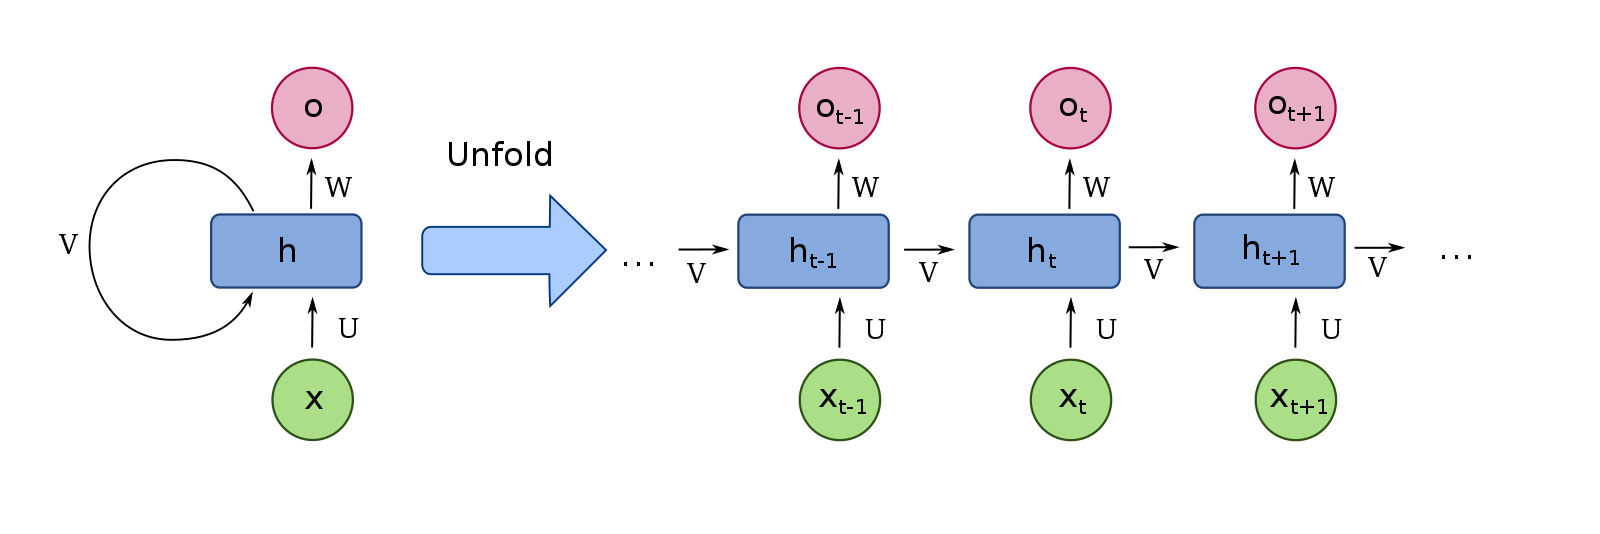
\includegraphics[scale = 0.15]{rnn-start.png}
\end{transitionframe}


\begin{frame}{Последовательности всюду}
\begin{center}
	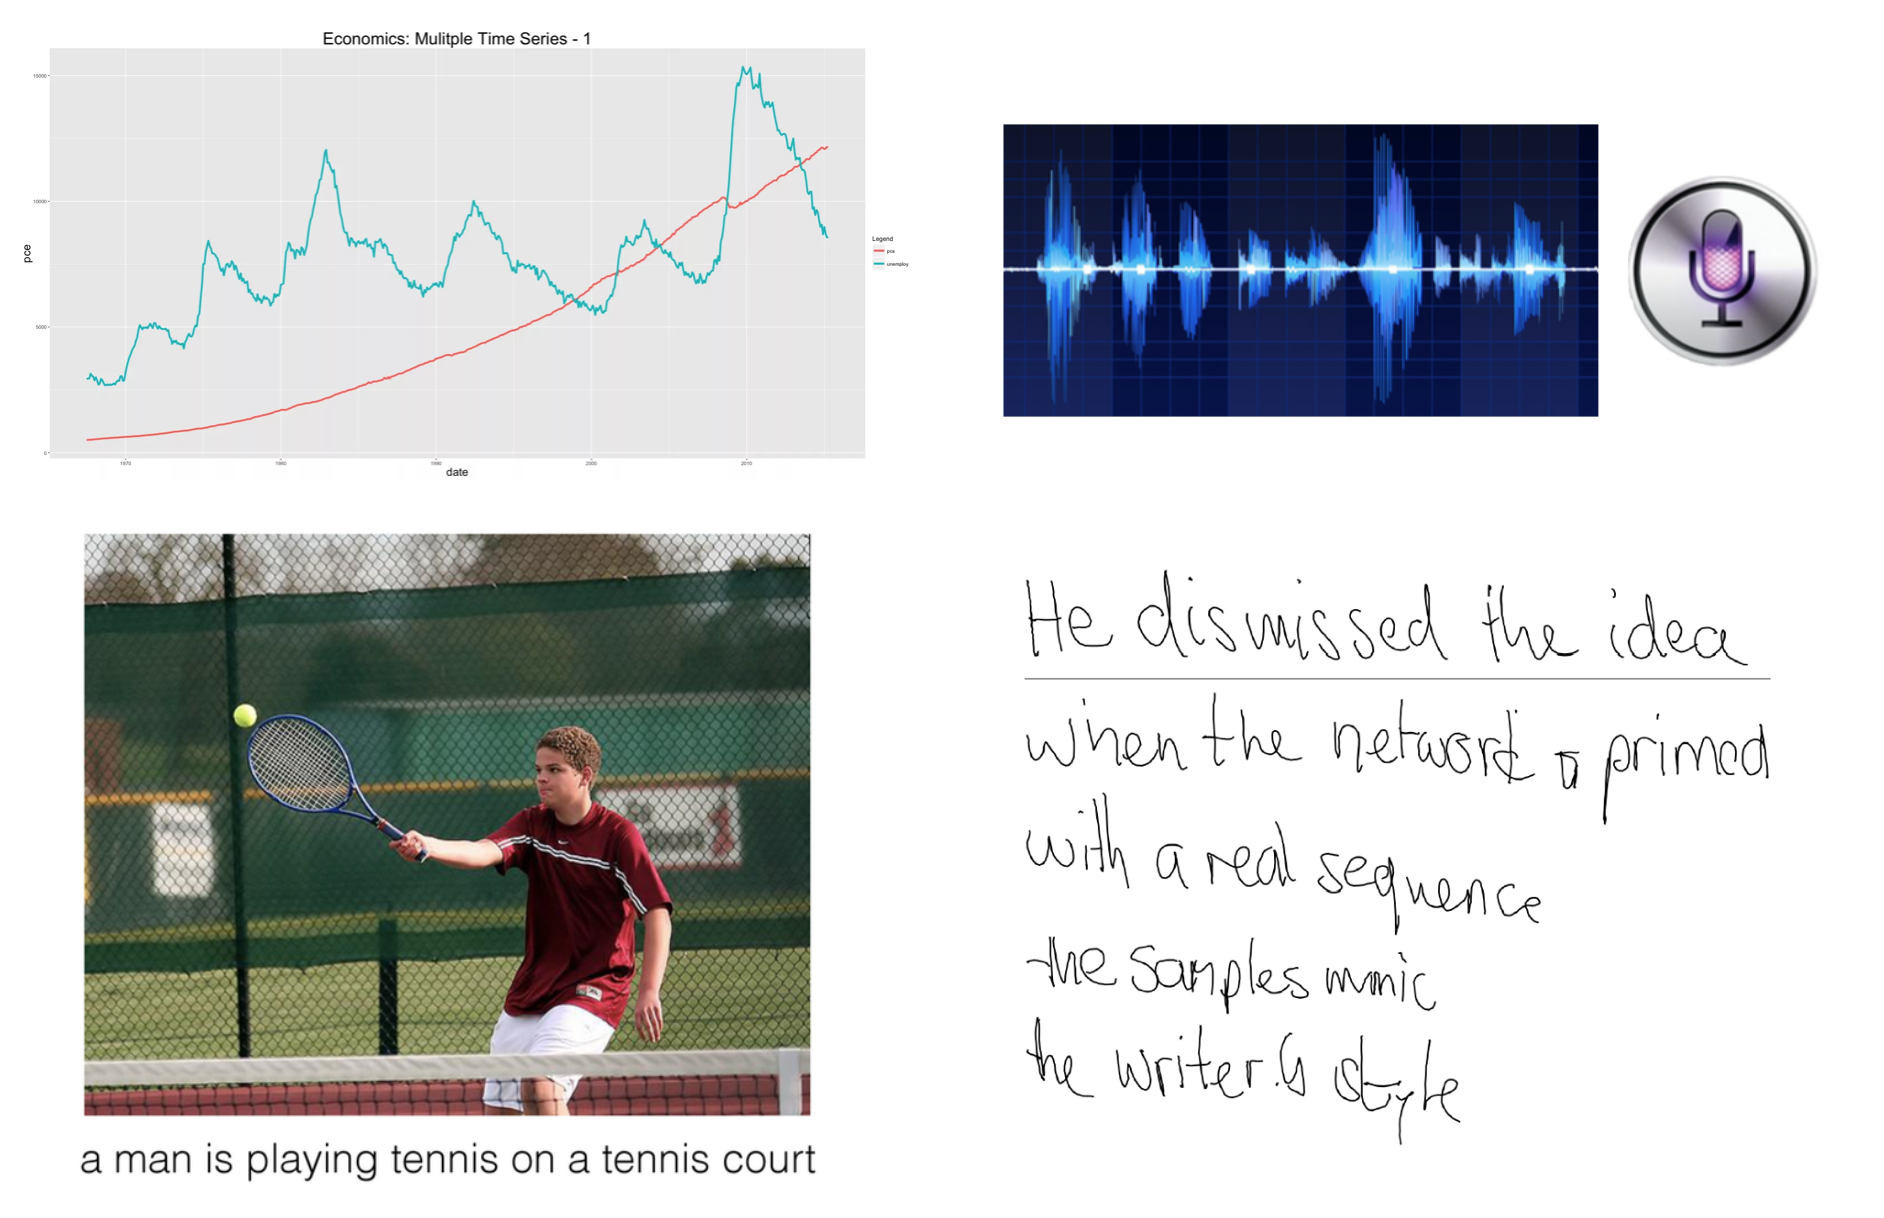
\includegraphics[width=.8\linewidth]{posled.png}
\end{center}
\end{frame}


\begin{frame}{Какой бывает работа с последовательностями}
\begin{center}
	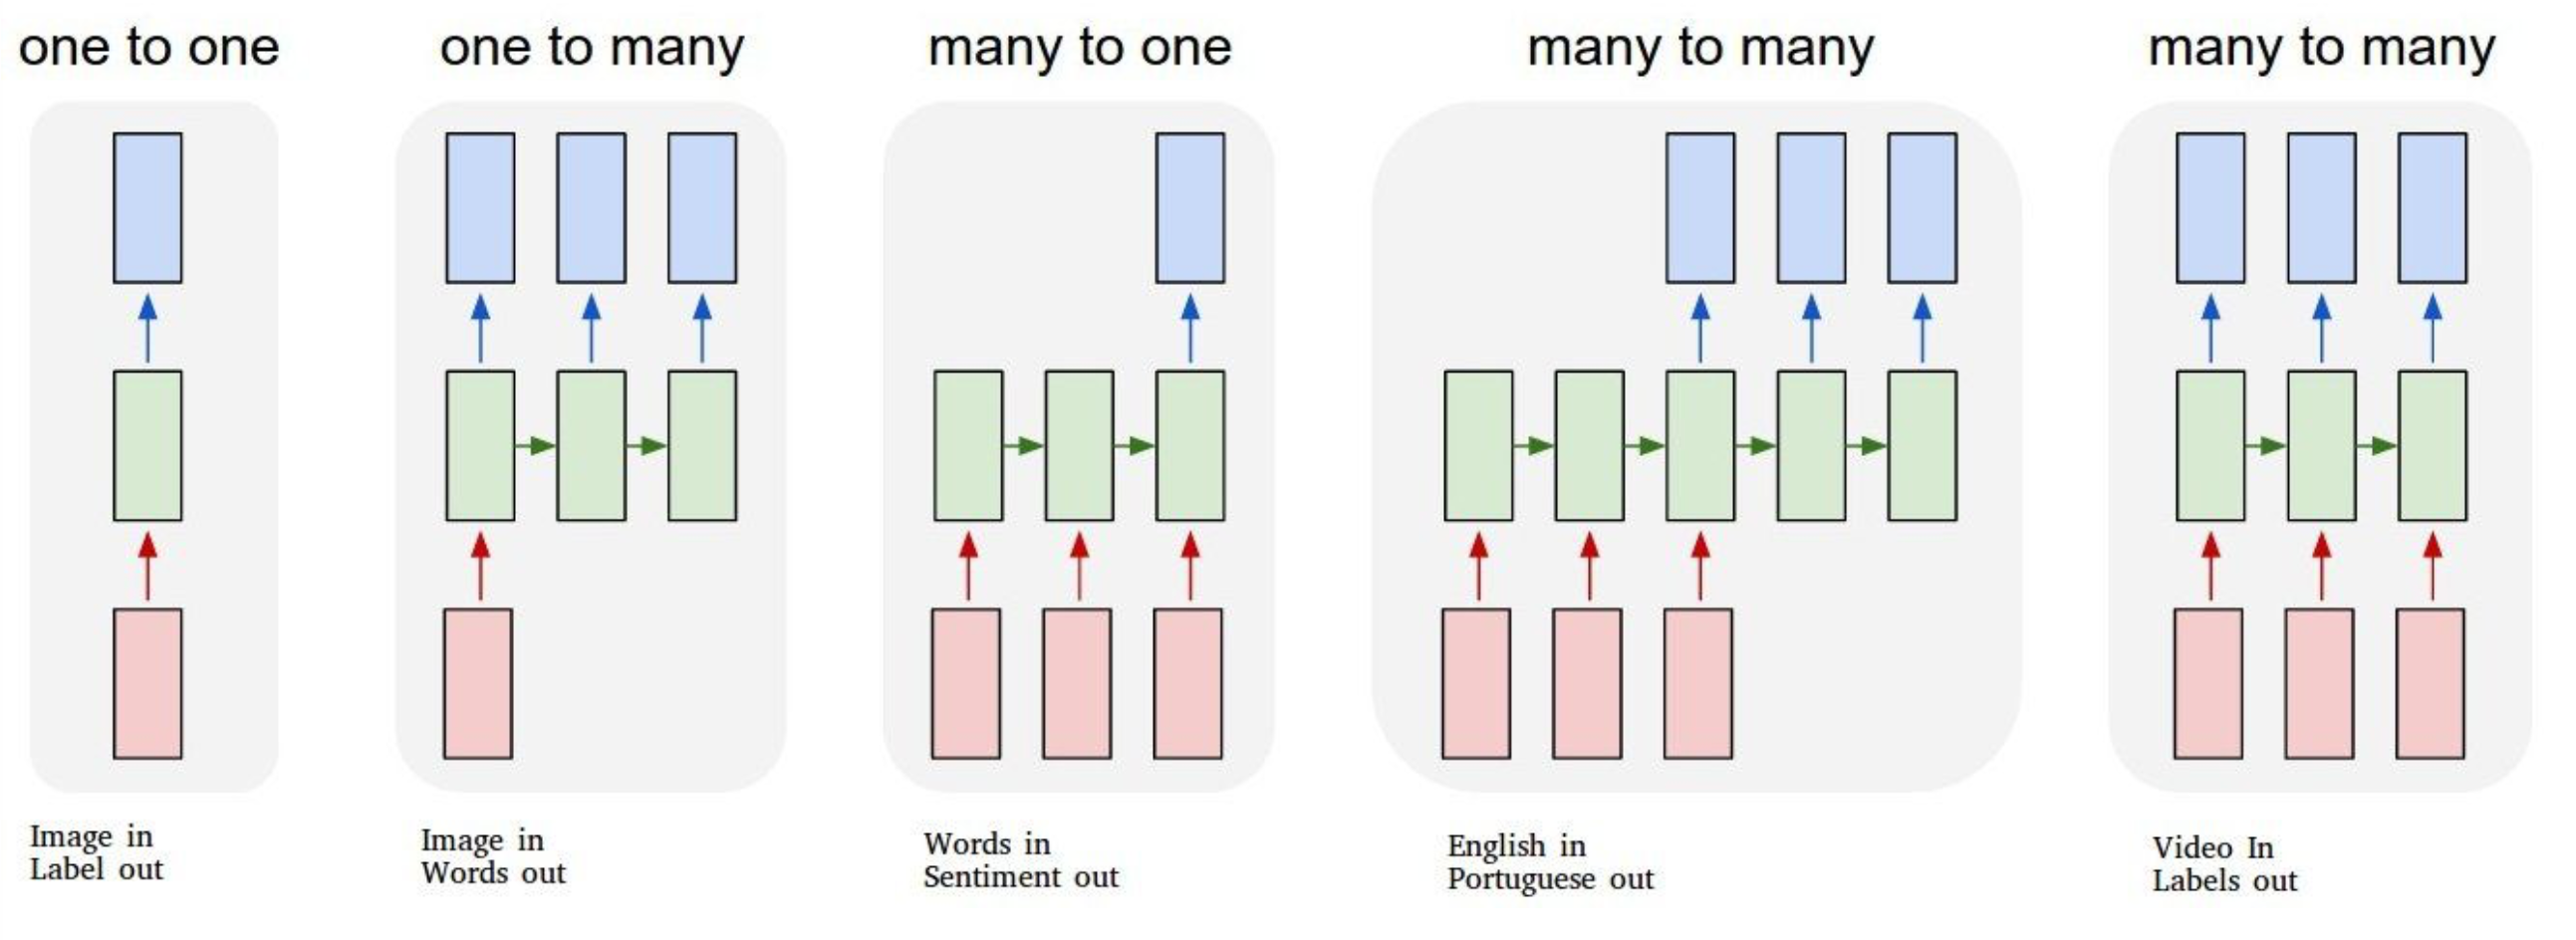
\includegraphics[width=.99\linewidth]{rnn_variants.png}
\end{center}

\vfill 
\footnotesize 
\color{blue} \url{https://karpathy.github.io/2015/05/21/rnn-effectiveness/} 
\end{frame}


\begin{frame}{От регрессии к нейрону}
\begin{columns}	
	\begin{column}{.35\linewidth}
		\begin{equation*} 
			\begin{aligned}
				y_i =& b + w \cdot x_i \\
				&\Downarrow \\
				h_i =& b + w \cdot x_i \\
				y_i = & f(h_i)
			\end{aligned}
		\end{equation*} 
	\end{column}
	\begin{column}{.64\linewidth}
		\begin{center}
			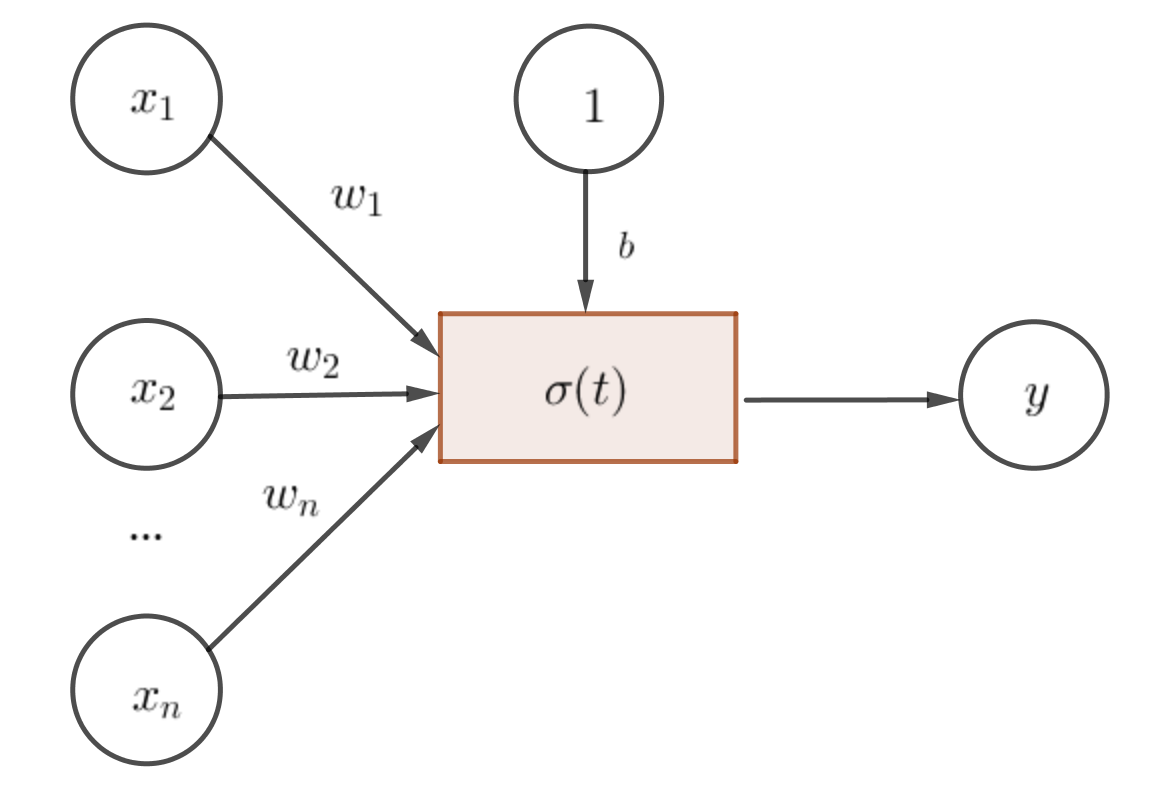
\includegraphics[width=.8\linewidth]{neuron_3.png}
		\end{center}
	\end{column}
\end{columns}
\end{frame}


\begin{frame}{От авторегрессии к нейрону}
\begin{columns}	
	\begin{column}{.68\linewidth}
		\begin{equation*} 
			y_t = b + w \cdot y_{t-1} 
		\end{equation*} 
	\end{column}
	\begin{column}{.28\linewidth}
	\begin{center}
	\definecolor{zzttqq}{rgb}{0.6,0.2,0.}
		\begin{tikzpicture}[scale=0.5]
		\fill[line width=2.pt,color=zzttqq,fill=zzttqq,fill opacity=0.10000000149011612] (2.,8.) -- (2.,6.) -- (4.,6.) -- (4.,8.) -- cycle;
		\draw  (3.,3.) circle (1.cm);
		\draw [color=zzttqq] (2.,8.)-- (2.,6.);
		\draw [color=zzttqq] (2.,6.)-- (4.,6.);
		\draw [color=zzttqq] (4.,6.)-- (4.,8.);
		\draw [color=zzttqq] (4.,8.)-- (2.,8.);
		\draw (3,11) circle (1.cm);
		\draw [->] (3,4) -- (3,6);
		\draw [->] (3,8) -- (3,10);
		\draw (2.1,3.7) node[anchor=north west] {$y_{t-1}$};
		\draw (2.2,11.6) node[anchor=north west] {$y_t$};
		\draw (1.8,9.7) node[anchor=north west] {$w$};
		\draw (1.8,5.6) node[anchor=north west] {$w$};
		\end{tikzpicture}
	\end{center}
	\end{column}
\end{columns}
\end{frame}


\begin{frame}{От авторегрессии к нейрону}
\begin{columns}
	\begin{column}{.68\linewidth}
		\begin{equation*} 
		\begin{aligned}
		y_t =& b + w \cdot y_{t-1}\\
		&\Downarrow \\
	   h_t =& f_h(b_h + w \cdot h_{t-1} + v \cdot y_{t-1})\\
	   y_t =& f_y(b_y + u \cdot h_t)
		\end{aligned}
		\end{equation*} 
	\end{column}
	\begin{column}{.28\linewidth}
	\begin{center}
		\definecolor{zzttqq}{rgb}{0.6,0.2,0.}
		\begin{tikzpicture}[scale=0.5]
			\fill[line width=2.pt,color=zzttqq,fill=zzttqq,fill opacity=0.10000000149011612] (2.,8.) -- (2.,6.) -- (4.,6.) -- (4.,8.) -- cycle;
			\draw  (3.,3.) circle (1.cm);
			\draw [color=zzttqq] (2.,8.)-- (2.,6.);
			\draw [color=zzttqq] (2.,6.)-- (4.,6.);
			\draw [color=zzttqq] (4.,6.)-- (4.,8.);
			\draw [color=zzttqq] (4.,8.)-- (2.,8.);
			\draw (3,11) circle (1.cm);
			\draw [->] (3,4) -- (3,6);
			\draw [->] (3,8) -- (3,10);
			\draw [shift={(4.45,7.)}]  plot[domain=-2.541806576912956:2.541806576912956,variable=\t]({1.*1.7715861960215864*cos(\t r)+0.*1.7715861960215864*sin(\t r)},{0.*1.7715861960215864*cos(\t r)+1.*1.7715861960215864*sin(\t r)});
			\draw (2.1,3.7) node[anchor=north west] {$y_{t-1}$};
			\draw (2.2,11.6) node[anchor=north west] {$y_t$};
			\draw (6.3,7.8) node[anchor=north west] {$w$};
			\draw (2.2,7.6) node[anchor=north west] {$h_t$};
			\draw (1.9,9.7) node[anchor=north west] {$u$};
			\draw (2,5.6) node[anchor=north west] {$v$};
		\end{tikzpicture}
	\end{center}
\end{column}	
\end{columns}
\end{frame}


\begin{frame}{От авторегрессии к нейрону}
\begin{columns}
	\begin{column}{.68\linewidth}
		\begin{equation*} 
		\begin{aligned}
		h_t =& f_h(b_h + w \cdot h_{t-1} + v \cdot \alert{x_t})\\
		y_t =& f_y(b_y + u \cdot h_t)
		\end{aligned}
		\end{equation*} 
	\end{column}
	\begin{column}{.28\linewidth}
		\begin{center}
			\definecolor{zzttqq}{rgb}{0.6,0.2,0.}
			\begin{tikzpicture}[scale=0.5]
				\fill[line width=2.pt,color=zzttqq,fill=zzttqq,fill opacity=0.10000000149011612] (2.,8.) -- (2.,6.) -- (4.,6.) -- (4.,8.) -- cycle;
				\draw  (3.,3.) circle (1.cm);
				\draw [color=zzttqq] (2.,8.)-- (2.,6.);
				\draw [color=zzttqq] (2.,6.)-- (4.,6.);
				\draw [color=zzttqq] (4.,6.)-- (4.,8.);
				\draw [color=zzttqq] (4.,8.)-- (2.,8.);
				\draw (3,11) circle (1.cm);
				\draw [->] (3,4) -- (3,6);
				\draw [->] (3,8) -- (3,10);
				\draw [shift={(4.45,7.)}]  plot[domain=-2.541806576912956:2.541806576912956,variable=\t]({1.*1.7715861960215864*cos(\t r)+0.*1.7715861960215864*sin(\t r)},{0.*1.7715861960215864*cos(\t r)+1.*1.7715861960215864*sin(\t r)});
				\draw (2.2,3.7) node[anchor=north west] {\alert{$x_{t}$}};
				\draw (2.2,11.6) node[anchor=north west] {$y_t$};
				\draw (6.3,7.8) node[anchor=north west] {$w$};
				\draw (2.2,7.6) node[anchor=north west] {$h_t$};
				\draw (1.9,9.7) node[anchor=north west] {$u$};
				\draw (2,5.6) node[anchor=north west] {$v$};
			\end{tikzpicture}
		\end{center}
	\end{column}	
\end{columns}
\end{frame}


\begin{frame}{Рекурентная сеть}
\begin{columns}
	\begin{column}{.18\linewidth}
		\begin{center}
			\definecolor{zzttqq}{rgb}{0.6,0.2,0.}
			\begin{tikzpicture}[scale=0.6]
					\fill[line width=2.pt,color=zzttqq,fill=zzttqq,fill opacity=0.10000000149011612] (2.,8.) -- (2.,6.) -- (4.,6.) -- (4.,8.) -- cycle;
					\draw  (3.,3.) circle (1.cm);
					\draw [color=zzttqq] (2.,8.)-- (2.,6.);
					\draw [color=zzttqq] (2.,6.)-- (4.,6.);
					\draw [color=zzttqq] (4.,6.)-- (4.,8.);
					\draw [color=zzttqq] (4.,8.)-- (2.,8.);
					\draw (3,11) circle (1.cm);
					\draw [->] (3,4) -- (3,6); 
					\draw [->] (3,8) -- (3,10);
					\draw [shift={(4.45,7.)}]  plot[domain=-2.541806576912956:2.541806576912956,variable=\t]({1.*1.7715861960215864*cos(\t r)+0.*1.7715861960215864*sin(\t r)},{0.*1.7715861960215864*cos(\t r)+1.*1.7715861960215864*sin(\t r)});
					\draw (2.4,3.5) node[anchor=north west] {$x_{t}$};
					\draw (2.4,11.5) node[anchor=north west] {$y_t$};
					\draw (6.3,7.8) node[anchor=north east] {$W$};
					\draw (2.4,7.6) node[anchor=north west] {$h_t$};
					\draw (1.9,9.7) node[anchor=north west] {$U$};
					\draw (2,5.6) node[anchor=north west] {$V$};
			\end{tikzpicture}
		\end{center}
	\end{column}
	\begin{column}{.1\linewidth}
		\centering
		 {\Huge \alert{$\Rightarrow$}} \\ \alert{Можно \\ перерисовать}
	\end{column}	
	\begin{column}{.69\linewidth}
		\begin{center}
		\begin{tikzpicture}
			\tikzstyle{place}=[circle, draw=black, minimum size = 12mm]
			\tikzstyle{placeh}=[minimum height=30pt,minimum width=30pt, inner sep=2pt, draw=black]
			
			\node at (-1.2,0.08) (here) {};
			
			\draw node at (0, 2) [place, fill=blue, opacity=0.1] (y) {$\hat y_{t-2}$};
			\draw node at (0, 2) [place] {$\hat y_{t-2}$};  % мои костыли максимально всратые
			\draw node at (0, 0) [placeh, fill=red, opacity=0.1] (h) {$h_{t-2}$};
			\draw node at (0, 0) [placeh] {$h_{t-2}$};
			\draw node at (0, -2) [place, fill=green, opacity=0.1] (x) {$x_{t-2}$};
			\draw node at (0, -2) [place] {$x_{t-2}$};
				
			\draw [->]  (here) to node[above]{$W$} (h);
			\draw [->]  (x) to node[left]{$V$} (h);
			\draw [->]  (h) to node[left]{$U$} (y);
			
			\draw node at (2, 2) [place, fill=blue, opacity=0.1] (y1) {$\hat y_{t-1}$};
			\draw node at (2, 2) [place] {$\hat y_{t-1}$};  % мои костыли максимально всратые
			\draw node at (2, 0) [placeh, fill=red, opacity=0.1] (h1) {$h_{t-1}$};
			\draw node at (2, 0) [placeh] {$h_{t-1}$};
			\draw node at (2, -2) [place, fill=green, opacity=0.1] (x1) {$x_{t-1}$};
			\draw node at (2, -2) [place] {$x_{t-1}$};
			
			\draw [->]  (h) to node[above]{$W$} (h1);
			\draw [->]  (x1) to node[left]{$V$} (h1);
			\draw [->]  (h1) to node[left]{$U$} (y1);
			
			\draw node at (4, 2) [place, fill=blue, opacity=0.1] (y2) {$\hat y_{t}$};
			\draw node at (4, 2) [place] {$\hat y_{t}$};  % мои костыли максимально всратые
			\draw node at (4, 0) [placeh, fill=red, opacity=0.1] (h2) {$h_{t}$};
			\draw node at (4, 0) [placeh] {$h_{t}$};
			\draw node at (4, -2) [place, fill=green, opacity=0.1] (x2) {$x_{t}$};
			\draw node at (4, -2) [place] {$x_{t}$};
			
			\draw [->]  (h1) to node[above]{$W$} (h2);
			\draw [->]  (x2) to node[left]{$V$} (h2);
			\draw [->]  (h2) to node[left]{$U$} (y2);
			
			
			\draw node at (6, 2) [place, fill=blue, opacity=0.1] (y3) {$\hat y_{t+1}$};
			\draw node at (6, 2) [place] {$\hat y_{t+1}$};  % мои костыли максимально всратые
			\draw node at (6, 0) [placeh, fill=red, opacity=0.1] (h3) {$h_{t+1}$};
			\draw node at (6, 0) [placeh] {$h_{t+1}$};
			\draw node at (6, -2) [place, fill=green, opacity=0.1] (x3) {$x_{t+1}$};
			\draw node at (6, -2) [place] {$x_{t+1}$};
			
			\draw [->]  (h2) to node[above]{$W$} (h3);
			\draw [->]  (x3) to node[left]{$V$} (h3);
			\draw [->]  (h3) to node[left]{$U$} (y3);
			
			\node at (7.2,0.08) (end) {};
			\draw [->]  (h3) to node[above]{$W$} (end);
		\end{tikzpicture}
	\end{center}
	\end{column}	
\end{columns}
\end{frame}



\begin{frame}{Рекурентная сеть}
		\begin{center}
	\begin{tikzpicture}
	\tikzstyle{place}=[circle, draw=black, minimum size = 12mm]
	\tikzstyle{placeh}=[minimum height=32pt,minimum width=32pt, inner sep=2pt, draw=black]
	
	\node at (-1.2,0.08) (here) {};
	
	\draw node at (0, 2) [place, fill=blue, opacity=0.1] (y) {$\hat y_{t-2}$};
	\draw node at (0, 2) [place] {$\hat y_{t-2}$};  % мои костыли максимально всратые
	\draw node at (0, 0) [placeh, fill=red, opacity=0.1] (h) {$h_{t-2}$};
	\draw node at (0, 0) [placeh] {$h_{t-2}$};
	\draw node at (0, -2) [place, fill=green, opacity=0.1] (x) {$x_{t-2}$};
	\draw node at (0, -2) [place] {$x_{t-2}$};
	
	\draw [->]  (here) to node[above]{$W$} (h);
	\draw [->]  (x) to node[left]{$V$} (h);
	\draw [->]  (h) to node[left]{$U$} (y);
	
	\draw node at (2, 2) [place, fill=blue, opacity=0.1] (y1) {$\hat y_{t-1}$};
	\draw node at (2, 2) [place] {$\hat y_{t-1}$};  % мои костыли максимально всратые
	\draw node at (2, 0) [placeh, fill=red, opacity=0.1] (h1) {$h_{t-1}$};
	\draw node at (2, 0) [placeh] {$h_{t-1}$};
	\draw node at (2, -2) [place, fill=green, opacity=0.1] (x1) {$x_{t-1}$};
	\draw node at (2, -2) [place] {$x_{t-1}$};
	
	\draw [->]  (h) to node[above]{$W$} (h1);
	\draw [->]  (x1) to node[left]{$V$} (h1);
	\draw [->]  (h1) to node[left]{$U$} (y1);
	
	\draw node at (4, 2) [place, fill=blue, opacity=0.1] (y2) {$\hat y_{t}$};
	\draw node at (4, 2) [place] {$\hat y_{t}$};  % мои костыли максимально всратые
	\draw node at (4, 0) [placeh, fill=red, opacity=0.1] (h2) {$h_{t}$};
	\draw node at (4, 0) [placeh] {$h_{t}$};
	\draw node at (4, -2) [place, fill=green, opacity=0.1] (x2) {$x_{t}$};
	\draw node at (4, -2) [place] {$x_{t}$};
	
	\draw [->]  (h1) to node[above]{$W$} (h2);
	\draw [->]  (x2) to node[left]{$V$} (h2);
	\draw [->]  (h2) to node[left]{$U$} (y2);
	
	
	\draw node at (6, 2) [place, fill=blue, opacity=0.1] (y3) {$\hat y_{t+1}$};
	\draw node at (6, 2) [place] {$\hat y_{t+1}$};  % мои костыли максимально всратые
	\draw node at (6, 0) [placeh, fill=red, opacity=0.1] (h3) {$h_{t+1}$};
	\draw node at (6, 0) [placeh] {$h_{t+1}$};
	\draw node at (6, -2) [place, fill=green, opacity=0.1] (x3) {$x_{t+1}$};
	\draw node at (6, -2) [place] {$x_{t+1}$};
	
	\draw [->]  (h2) to node[above]{$W$} (h3);
	\draw [->]  (x3) to node[left]{$V$} (h3);
	\draw [->]  (h3) to node[left]{$U$} (y3);
	
	\node at (7.2,0.08) (end) {};
	\draw [->]  (h3) to node[above]{$W$} (end);
	\end{tikzpicture}
\end{center}

\[
h_t = f_h( V x_t + W h_{t-1} + b_h) \qquad \hat y_t = f_y ( U h_t + b_y)
\]

\vfill
\small \centering
\alert{Рекуррентную сеть можно рассматривать, как несколько копий одной и той же сети, каждая из которых передает информацию последующей копии. }
\end{frame}


\begin{frame}{Рекурентная сеть}
\begin{wideitemize} 
	\item  На вход поступает последовательность (текст, видео, картинка, временной ряд)
	\item  Нейрон просматривает её, на каждом шаге он взаимодействует сам собой и с последовательностью 
	\item \alert{На каждом шаге нейрон использует одни и те же функции активации и веса}
	\item Можно сказать, что у RNN есть память (скрытое состояние $h_t$), в которой хранится информация о предыдущих элементах последовательности
\end{wideitemize} 
\end{frame}


\begin{frame}{Пример: языковая модель}
		\begin{columns}
		\begin{column}{.4\linewidth}
			\begin{wideitemize} 
				\item  Буквенная языковая модель (character-level Language Model)
				\item Словарь:  [h,e,l,o]
				\item Пытаемся выучить слово “hello”
			\end{wideitemize}
		\end{column}	
		\begin{column}{.7\linewidth}			
		\begin{center}
			\only<1>{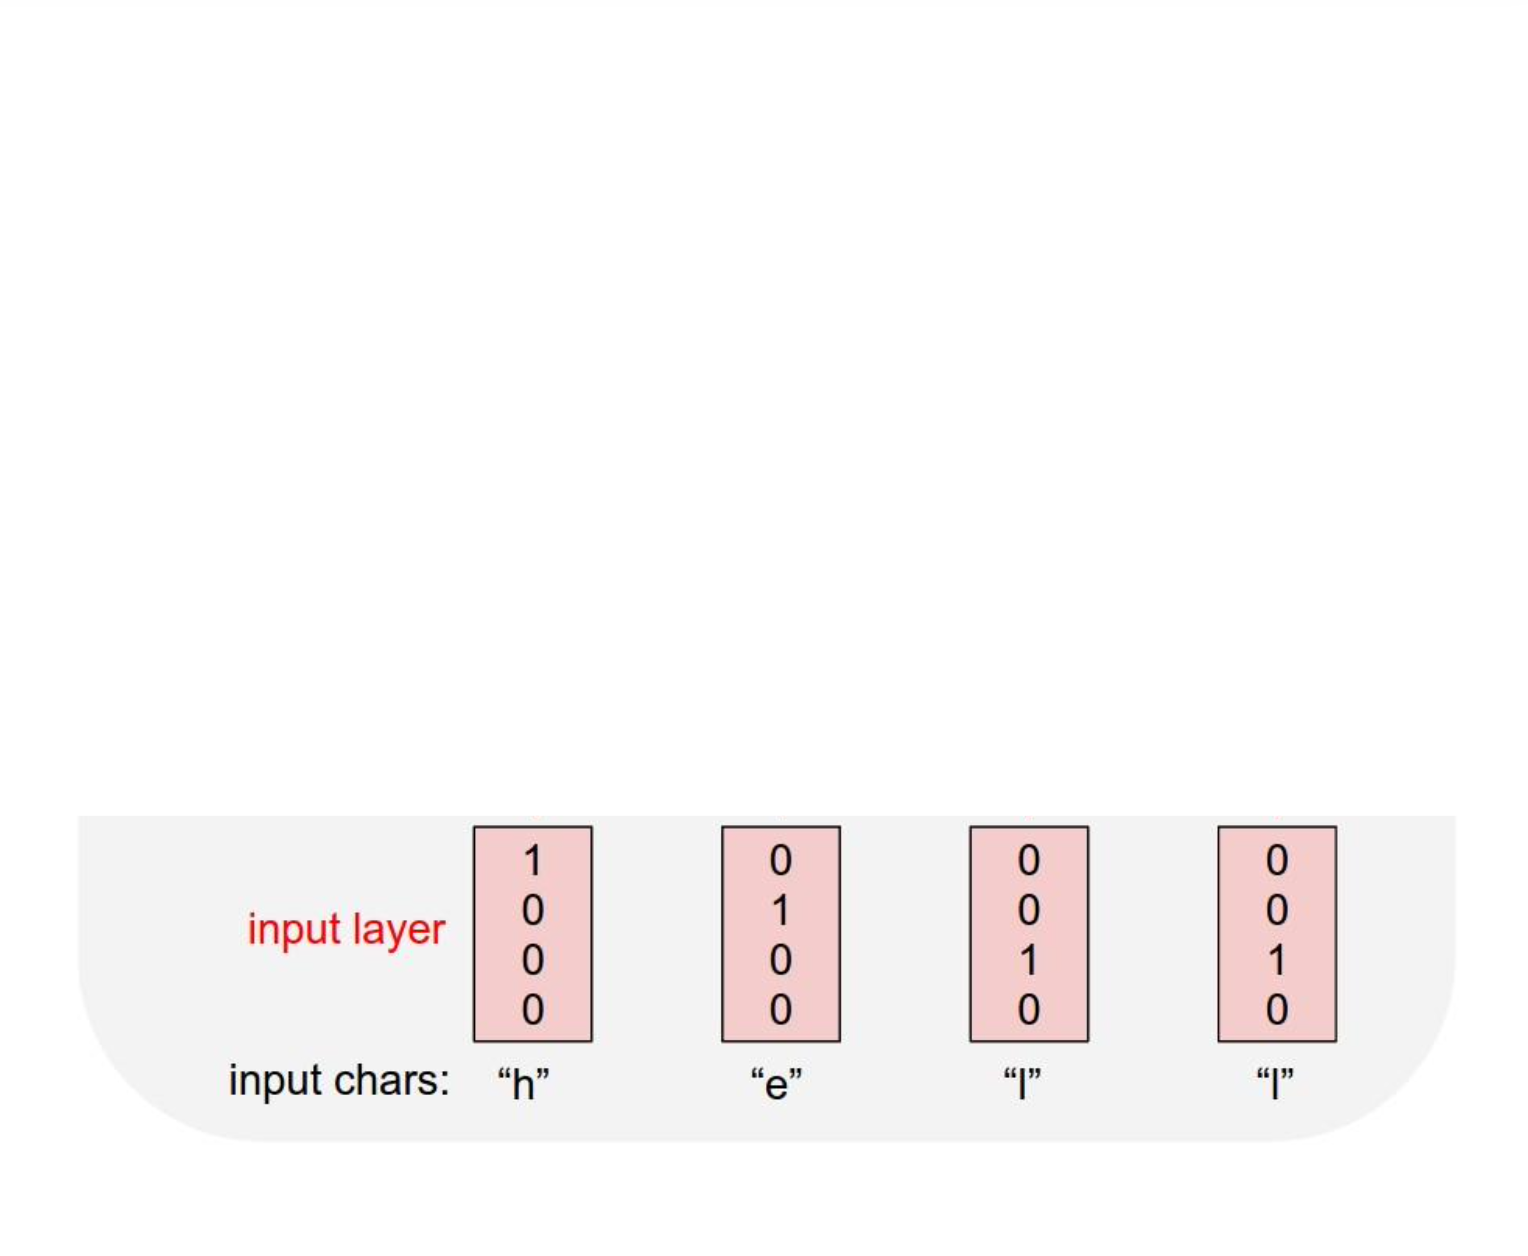
\includegraphics[width=.8\linewidth]{lang_model1.png}}
			\only<2>{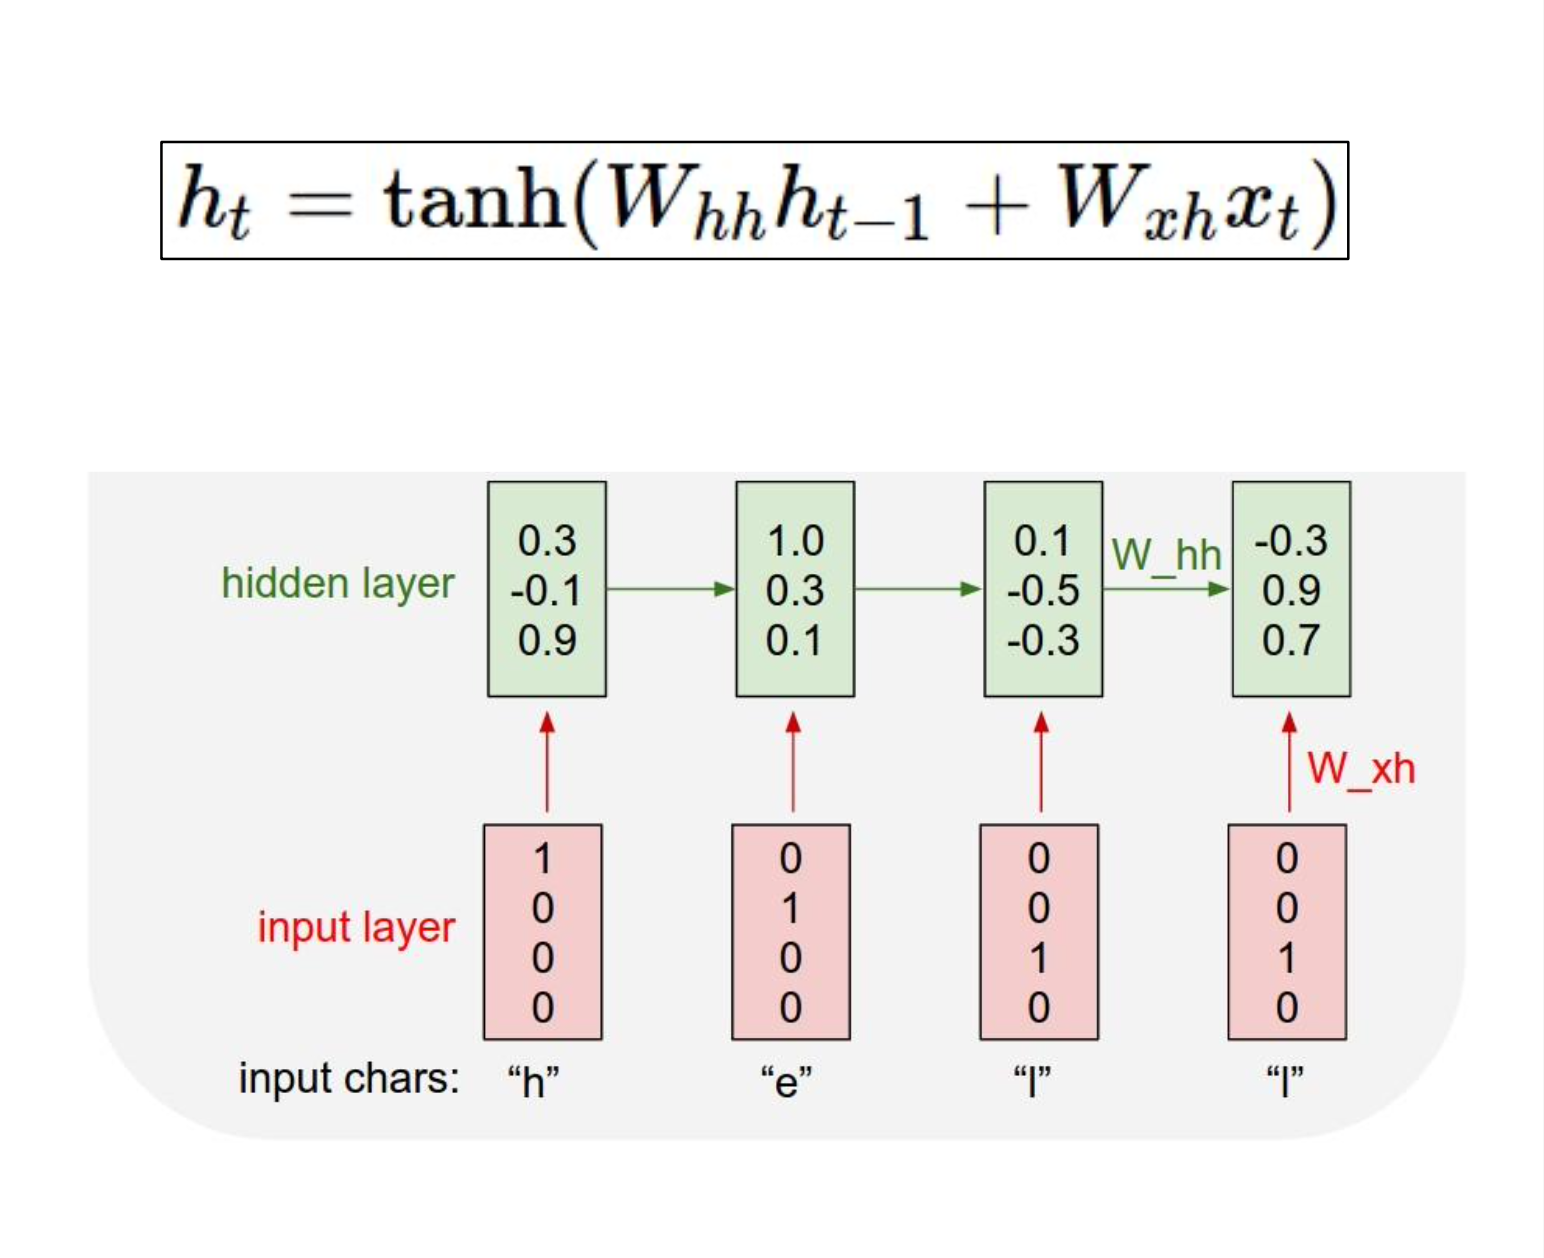
\includegraphics[width=.8\linewidth]{lang_model2.png}}
			\only<3>{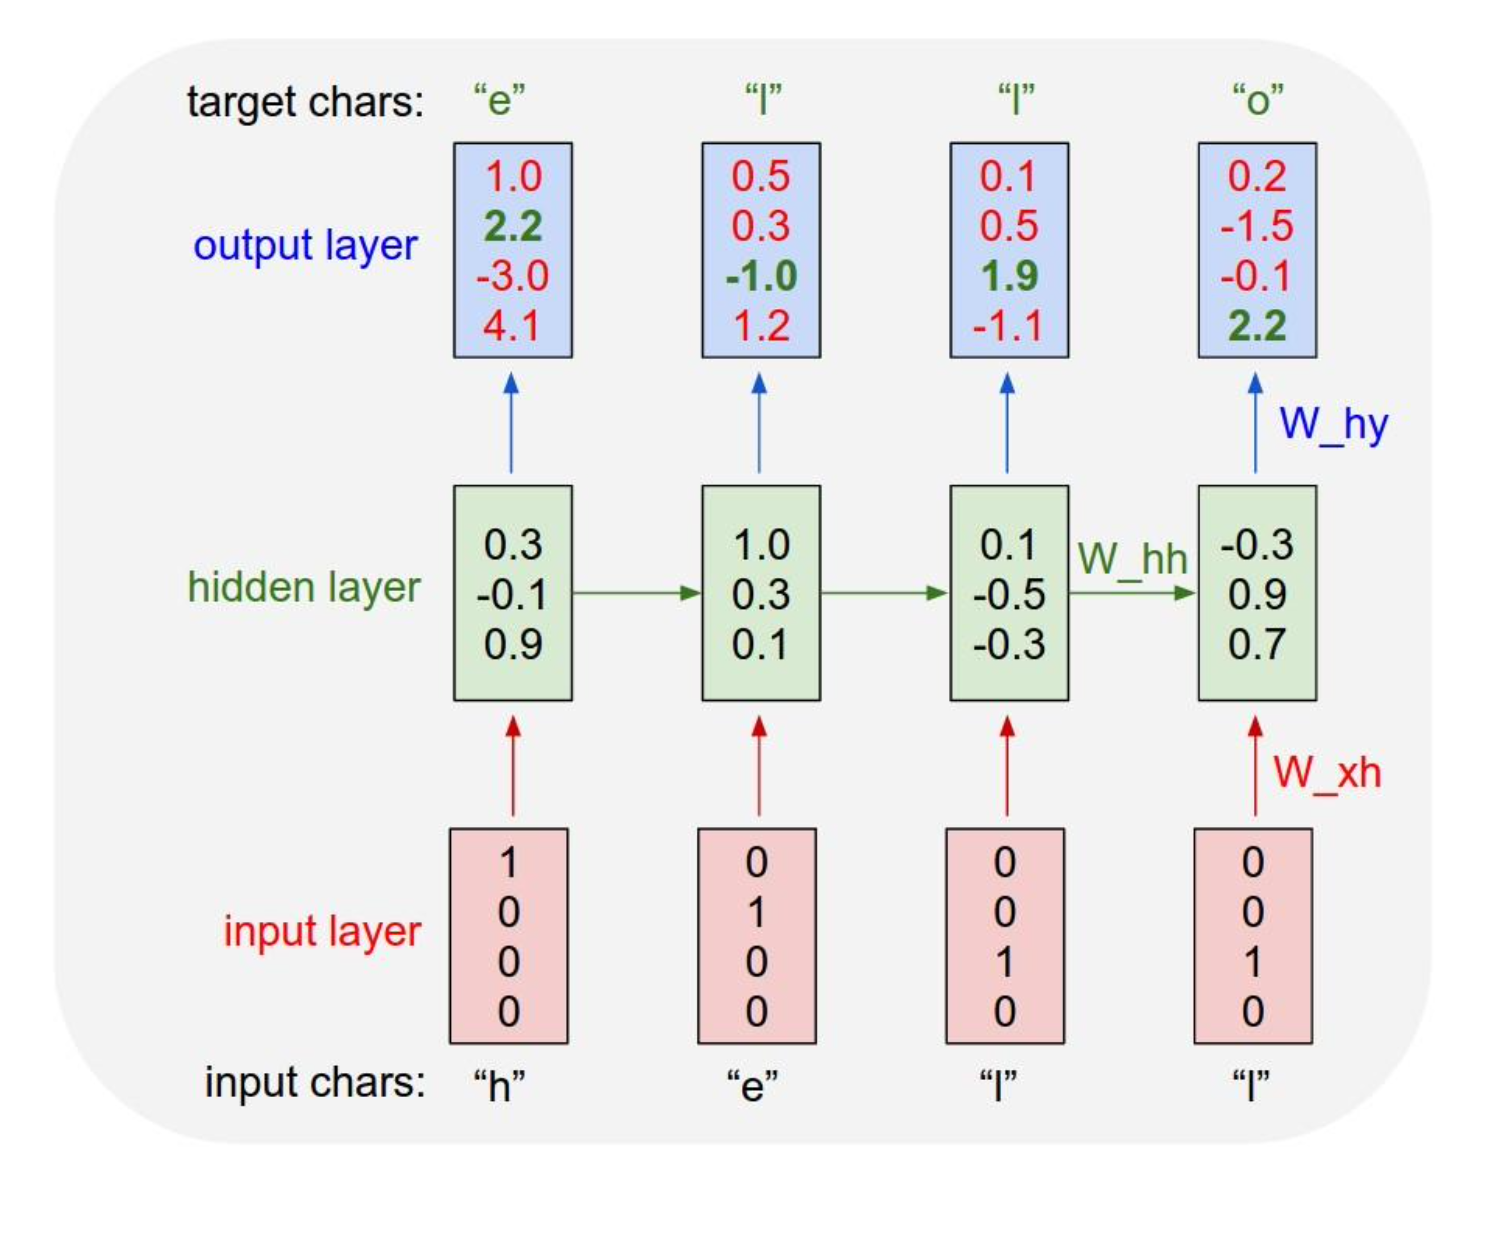
\includegraphics[width=.8\linewidth]{lang_model3.png}}
		\end{center}
		\end{column}	
		\end{columns}
\vfill 
\footnotesize 
\color{blue} \url{https://karpathy.github.io/2015/05/21/rnn-effectiveness/} 
\end{frame}


\begin{frame}{Пример: языковая модель}
\begin{columns}
	\begin{column}{.4\linewidth}
		\begin{wideitemize} 
			\item  Буквенная языковая модель (character-level Language Model)
			\item Словарь:  [h,e,l,o]
			\item В тестовом режиме предсказываем следующие буквы
		\end{wideitemize}
	\end{column}	
	\begin{column}{.7\linewidth}			
		\begin{center}
			\only<1>{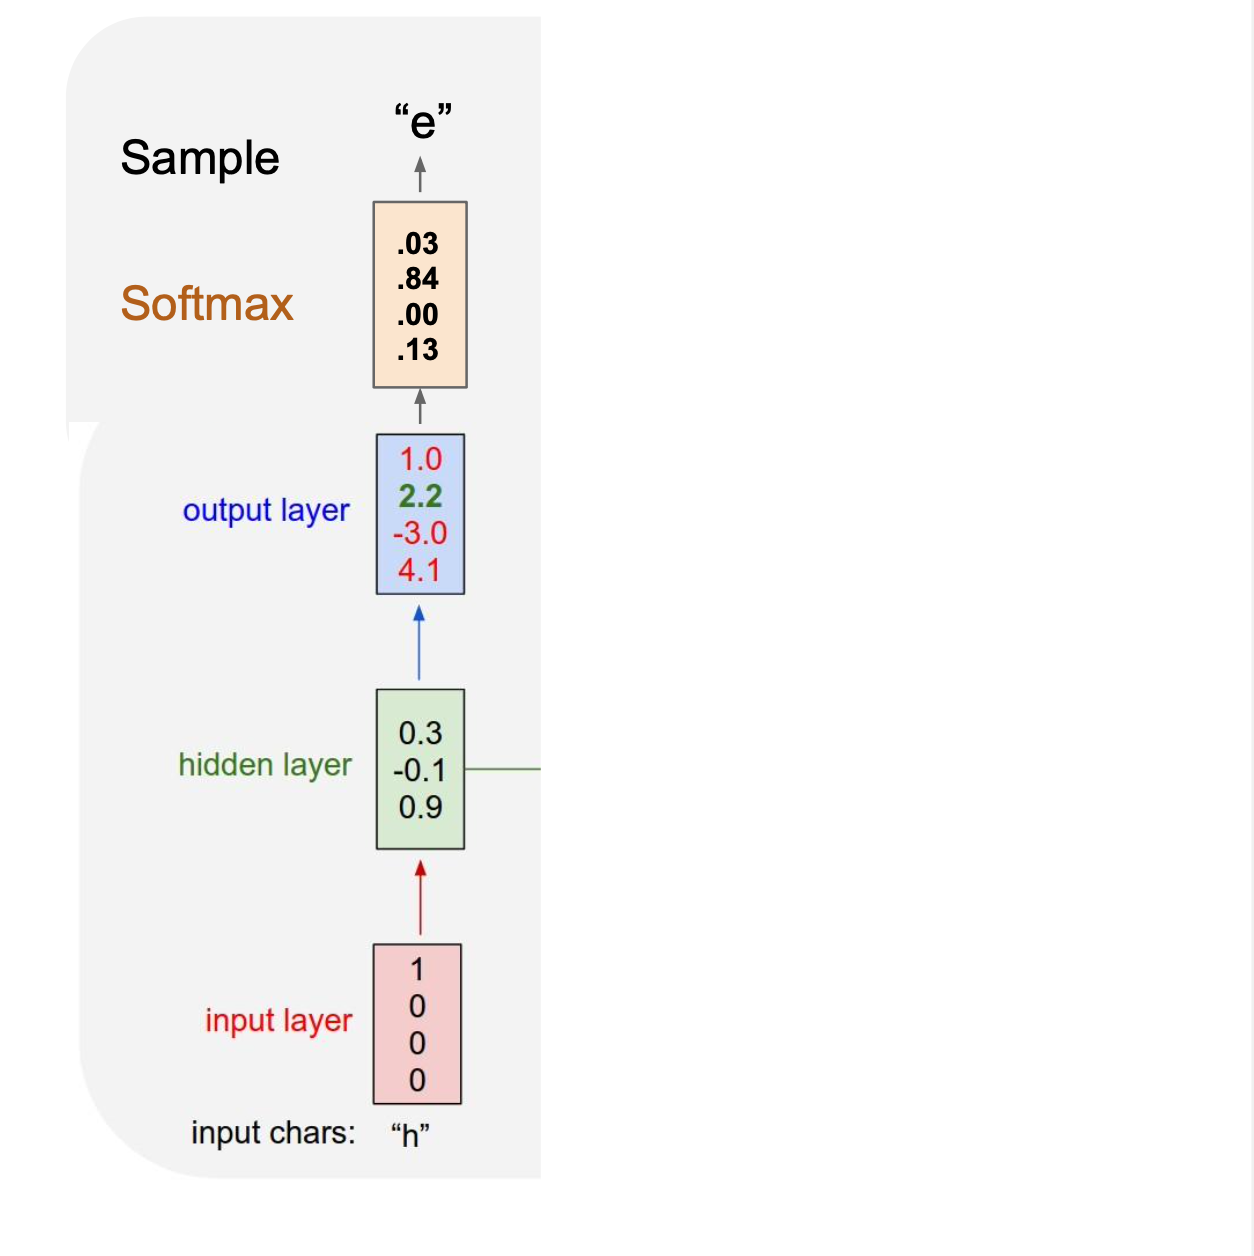
\includegraphics[width=.6\linewidth]{lang_model4.png}}
			\only<2>{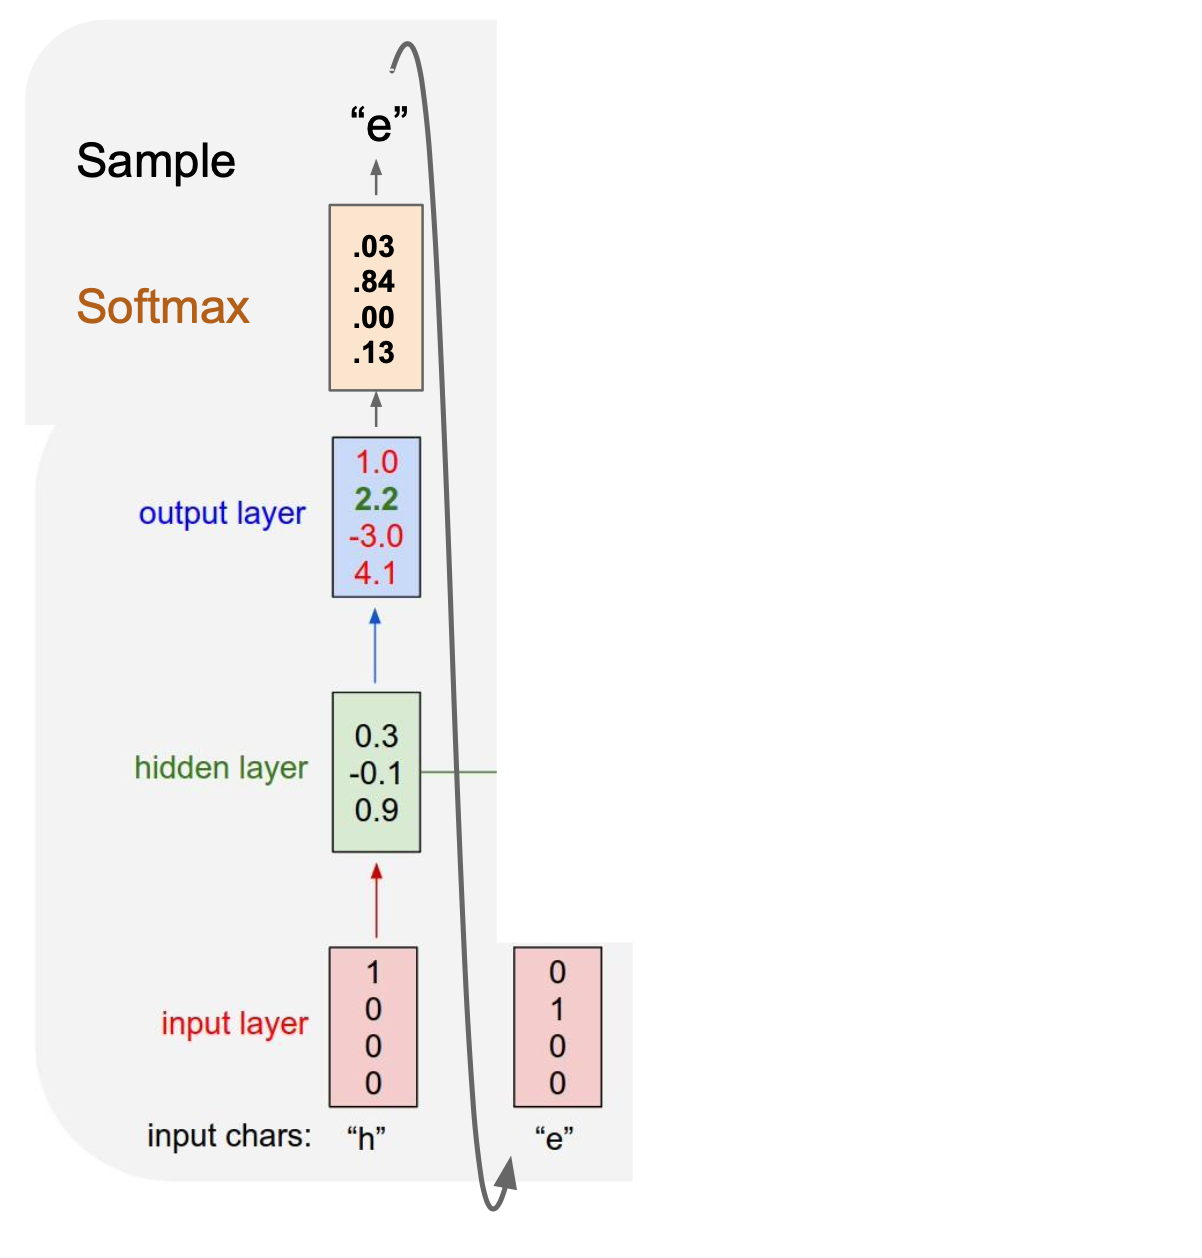
\includegraphics[width=.6\linewidth]{lang_model5.png}}
			\only<3>{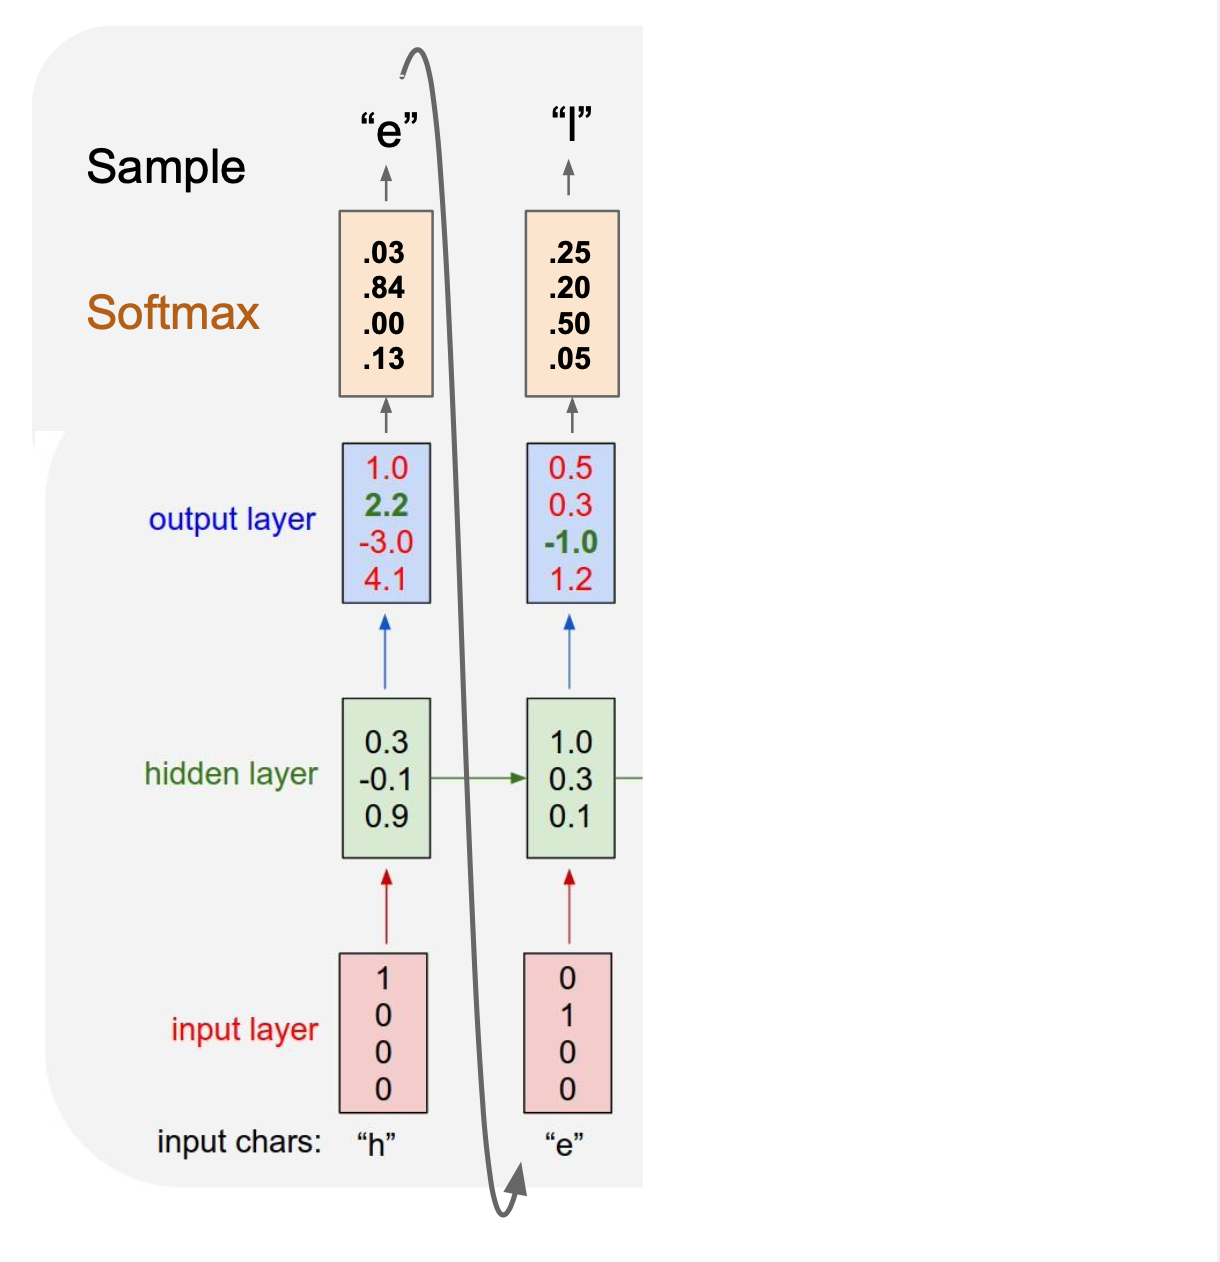
\includegraphics[width=.6\linewidth]{lang_model6.png}}
			\only<4>{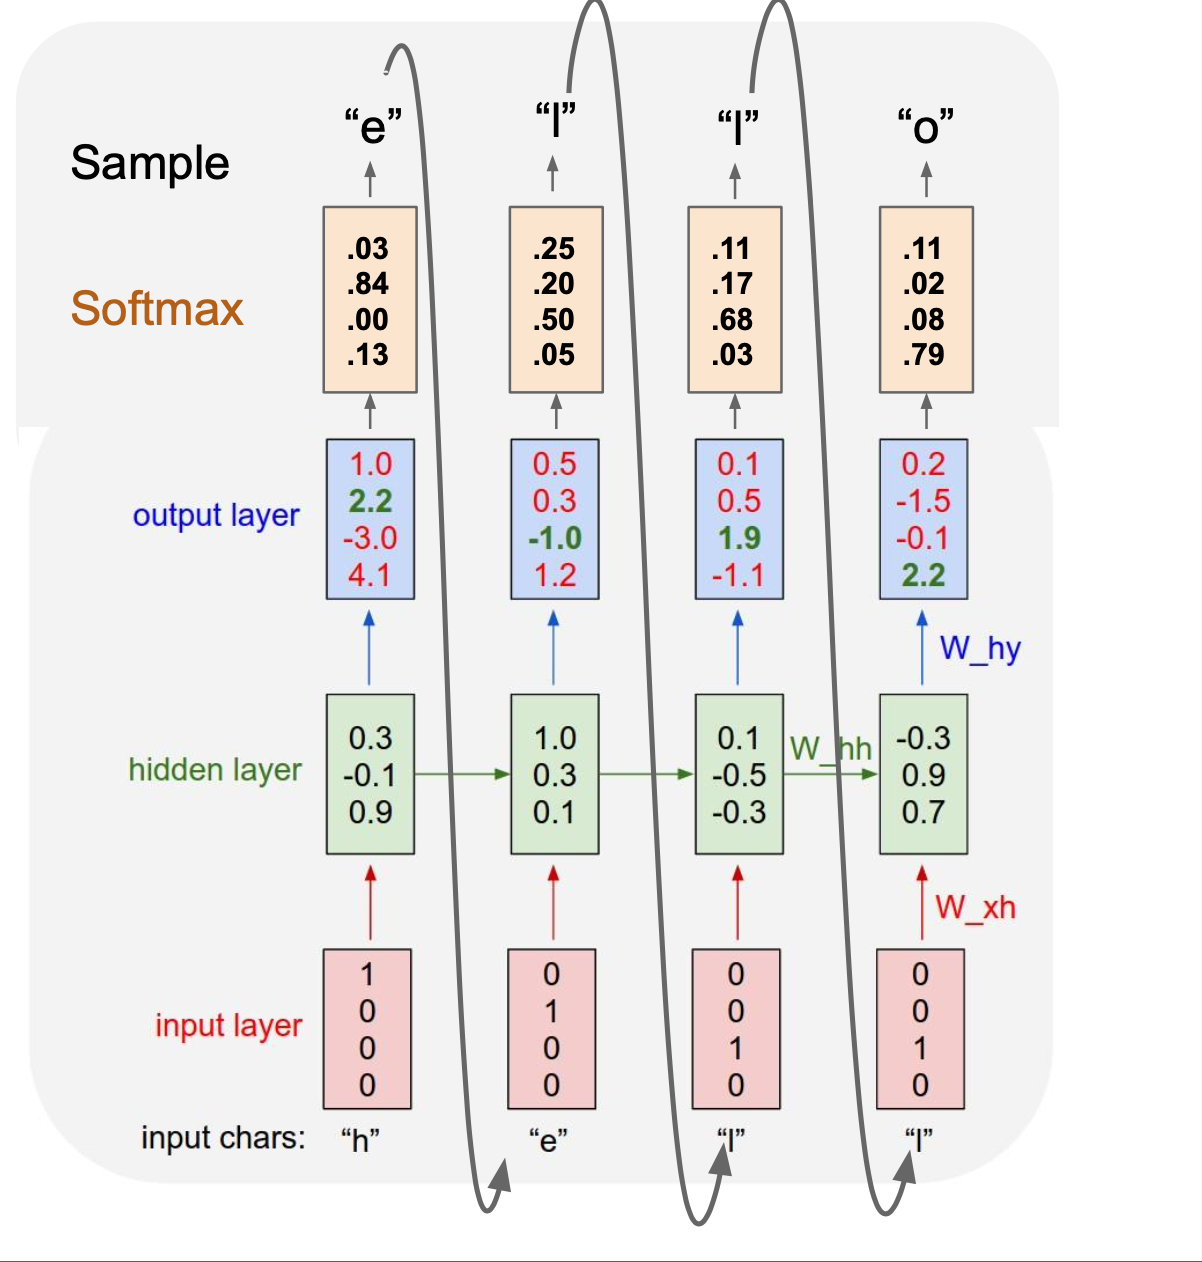
\includegraphics[width=.6\linewidth]{lang_model7.png}}
		\end{center}
	\end{column}	
\end{columns}
\vfill 
\footnotesize 
\color{blue} \url{https://karpathy.github.io/2015/05/21/rnn-effectiveness/} 
\end{frame}


\begin{frame}{Злобный нейрон}
\begin{center}
	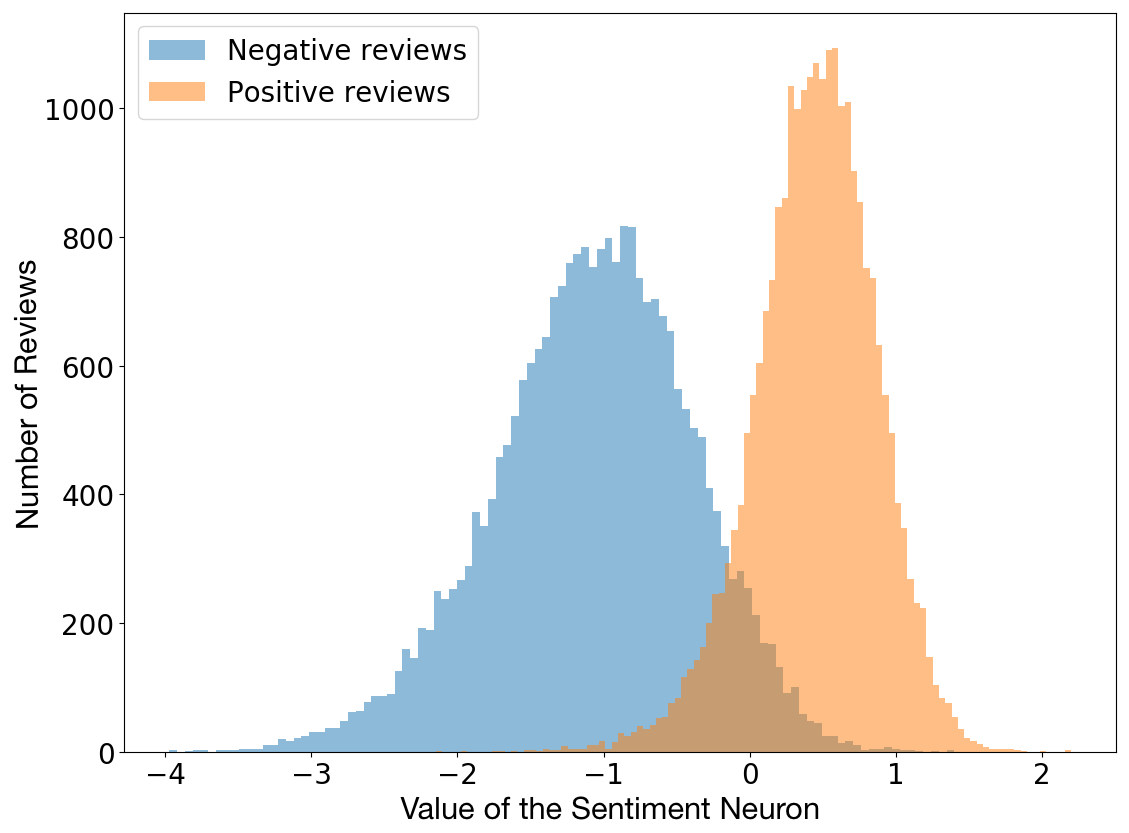
\includegraphics[width=.6\linewidth]{sent_neuron.png}
\end{center}
\vfill 
\footnotesize 
\color{blue} \url{https://openai.com/blog/unsupervised-sentiment-neuron/} 
\end{frame}


\begin{frame}{Злобный нейрон}
\begin{center}
	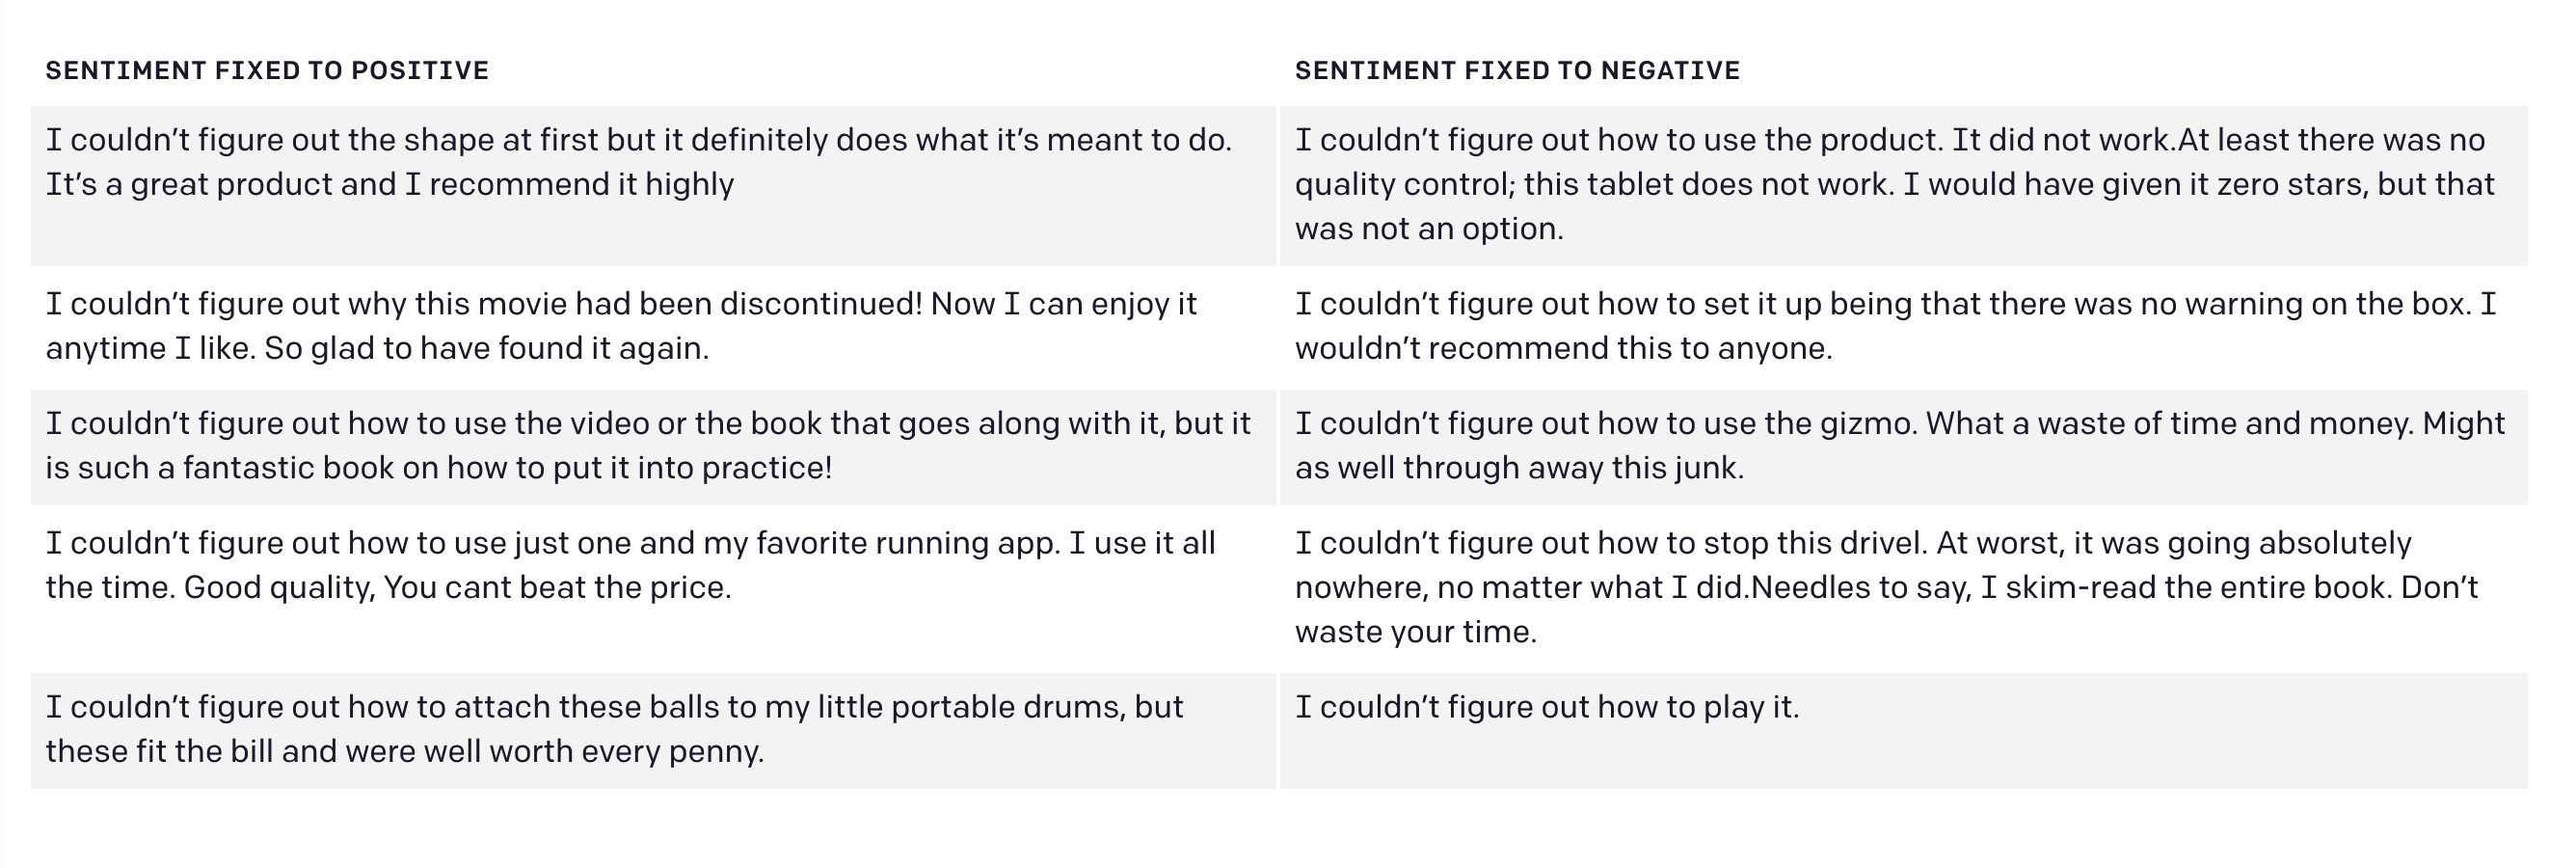
\includegraphics[width=.99\linewidth]{sent-text.png}
\end{center}
\vfill 
\footnotesize 
\color{blue} \url{https://openai.com/blog/unsupervised-sentiment-neuron/} 
\end{frame}





\begin{frame}{Backpropagation through time}
\begin{wideitemize} 
	\item  \alert{Проблема} состоит в том, что в работе сетки появилось \alert{новое измерение: время} 
	
	\item На каждом шаге сетка взвешивает свой предыдущий опыт и новую информацию, получается, что при обучении, мы должны брать производную назад во времени
\end{wideitemize} 
\end{frame}


\begin{transitionframe}
	\begin{center}
		\Huge Backpropagation through time
	\end{center}
	\centering 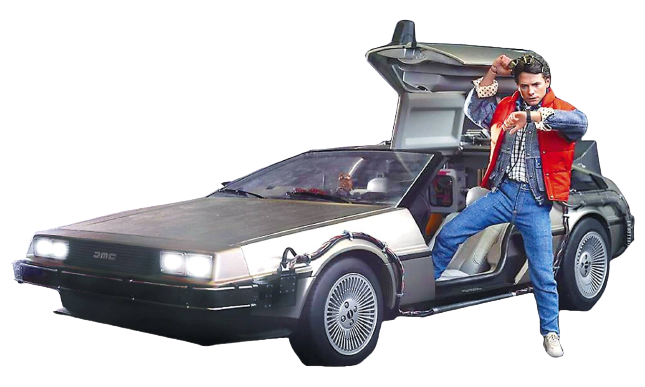
\includegraphics[scale = 0.25]{future.png}
\end{transitionframe}



\begin{frame}{Backpropagation through time}
\begin{columns}
	\begin{column}{.48\linewidth}
		\only<1>{
		\begin{wideitemize} 
			\item $y_t$ — настоящее значение
			\item $\hat{y_t}$  — прогноз
			\item $L_t(y_t, \hat{y_t})$ —  функция потерь
			\item $L = \sum_{t} L_t(y_t, \hat{y_t}) $ — ошибка по всей последовательности
		\end{wideitemize} }
	{\large \only<2>{\color{blue} Forward pass: \\ $\qquad h_t, \hat{y}_t, L_t, L$}}
	\end{column}
	\begin{column}{.48\linewidth}
		\begin{center}
		\begin{tikzpicture}
				\tikzstyle{place}=[circle, draw=black, minimum size = 12mm]
				\tikzstyle{placeh}=[minimum height=32pt,minimum width=32pt, inner sep=2pt, draw=black]
				
				\node at (-1.2,0.08) (here) {};
				
				\draw node at (0, 2) [place, fill=blue, opacity=0.1] (y) {$\hat y_{t-2}$};
				\draw node at (0, 2) [place] {$\hat y_{t-2}$};  % мои костыли максимально всратые
				\draw node at (0, 0) [placeh, fill=red, opacity=0.1] (h) {$h_{t-2}$};
				\draw node at (0, 0) [placeh] {$h_{t-2}$};
				\draw node at (0, -2) [place, fill=green, opacity=0.1] (x) {$x_{t-2}$};
				\draw node at (0, -2) [place] {$x_{t-2}$};
				
				\draw [->]  (here) to (h);
				\draw [->]  (x) to node[left]{$V$} (h);
				\draw [->]  (h) to node[left]{$U$} (y);
				
				\draw node at (2, 2) [place, fill=blue, opacity=0.1] (y1) {$\hat y_{t-1}$};
				\draw node at (2, 2) [place] {$\hat y_{t-1}$};  % мои костыли максимально всратые
				\draw node at (2, 0) [placeh, fill=red, opacity=0.1] (h1) {$h_{t-1}$};
				\draw node at (2, 0) [placeh] {$h_{t-1}$};
				\draw node at (2, -2) [place, fill=green, opacity=0.1] (x1) {$x_{t-1}$};
				\draw node at (2, -2) [place] {$x_{t-1}$};
				
				\draw [->]  (h) to node[above]{$W$} (h1);
				\draw [->]  (x1) to node[left]{$V$} (h1);
				\draw [->]  (h1) to node[left]{$U$} (y1);
				
				\draw node at (4, 2) [place, fill=blue, opacity=0.1] (y2) {$\hat y_{t}$};
				\draw node at (4, 2) [place] {$\hat y_{t}$};  % мои костыли максимально всратые
				\draw node at (4, 0) [placeh, fill=red, opacity=0.1] (h2) {$h_{t}$};
				\draw node at (4, 0) [placeh] {$h_{t}$};
				\draw node at (4, -2) [place, fill=green, opacity=0.1] (x2) {$x_{t}$};
				\draw node at (4, -2) [place] {$x_{t}$};
				
				\draw [->]  (h1) to node[above]{$W$} (h2);
				\draw [->]  (x2) to node[left]{$V$} (h2);
				\draw [->]  (h2) to node[left]{$U$} (y2);

				\node at (5.2,0.08) (end) {};
				\draw [->]  (h2) to node[above]{$W$} (end);
				
				\draw node at (4, 3.5)  (l2){$L_{t}$}; 
				\draw node at (2, 3.5)  (l1){$L_{t-1}$};
				\draw node at (0, 3.5)  (l){$L_{t-2}$};
				\draw node at (2, 4.5)  (sl){$L$};
				\draw [->]  (y) to  (l);
				\draw [->]  (y1) to  (l1);
				\draw [->]  (y2) to  (l2);		
				\draw [->]  (l) to  (sl);	
				\draw [->]  (l1) to  (sl);	
				\draw [->]  (l2) to  (sl);
				
				\only<2>{\draw [->, blue, line width=2.pt]  (-1.2, -2.65) to  (5.2,-2.65); }
				\only<2>{\draw [->, blue, line width=2.pt]  (5.4, -2) to  (5.4, 4.2); }
		\end{tikzpicture}
		\end{center}
	\end{column}	
\end{columns}
\end{frame}


\begin{frame}
\begin{center}
	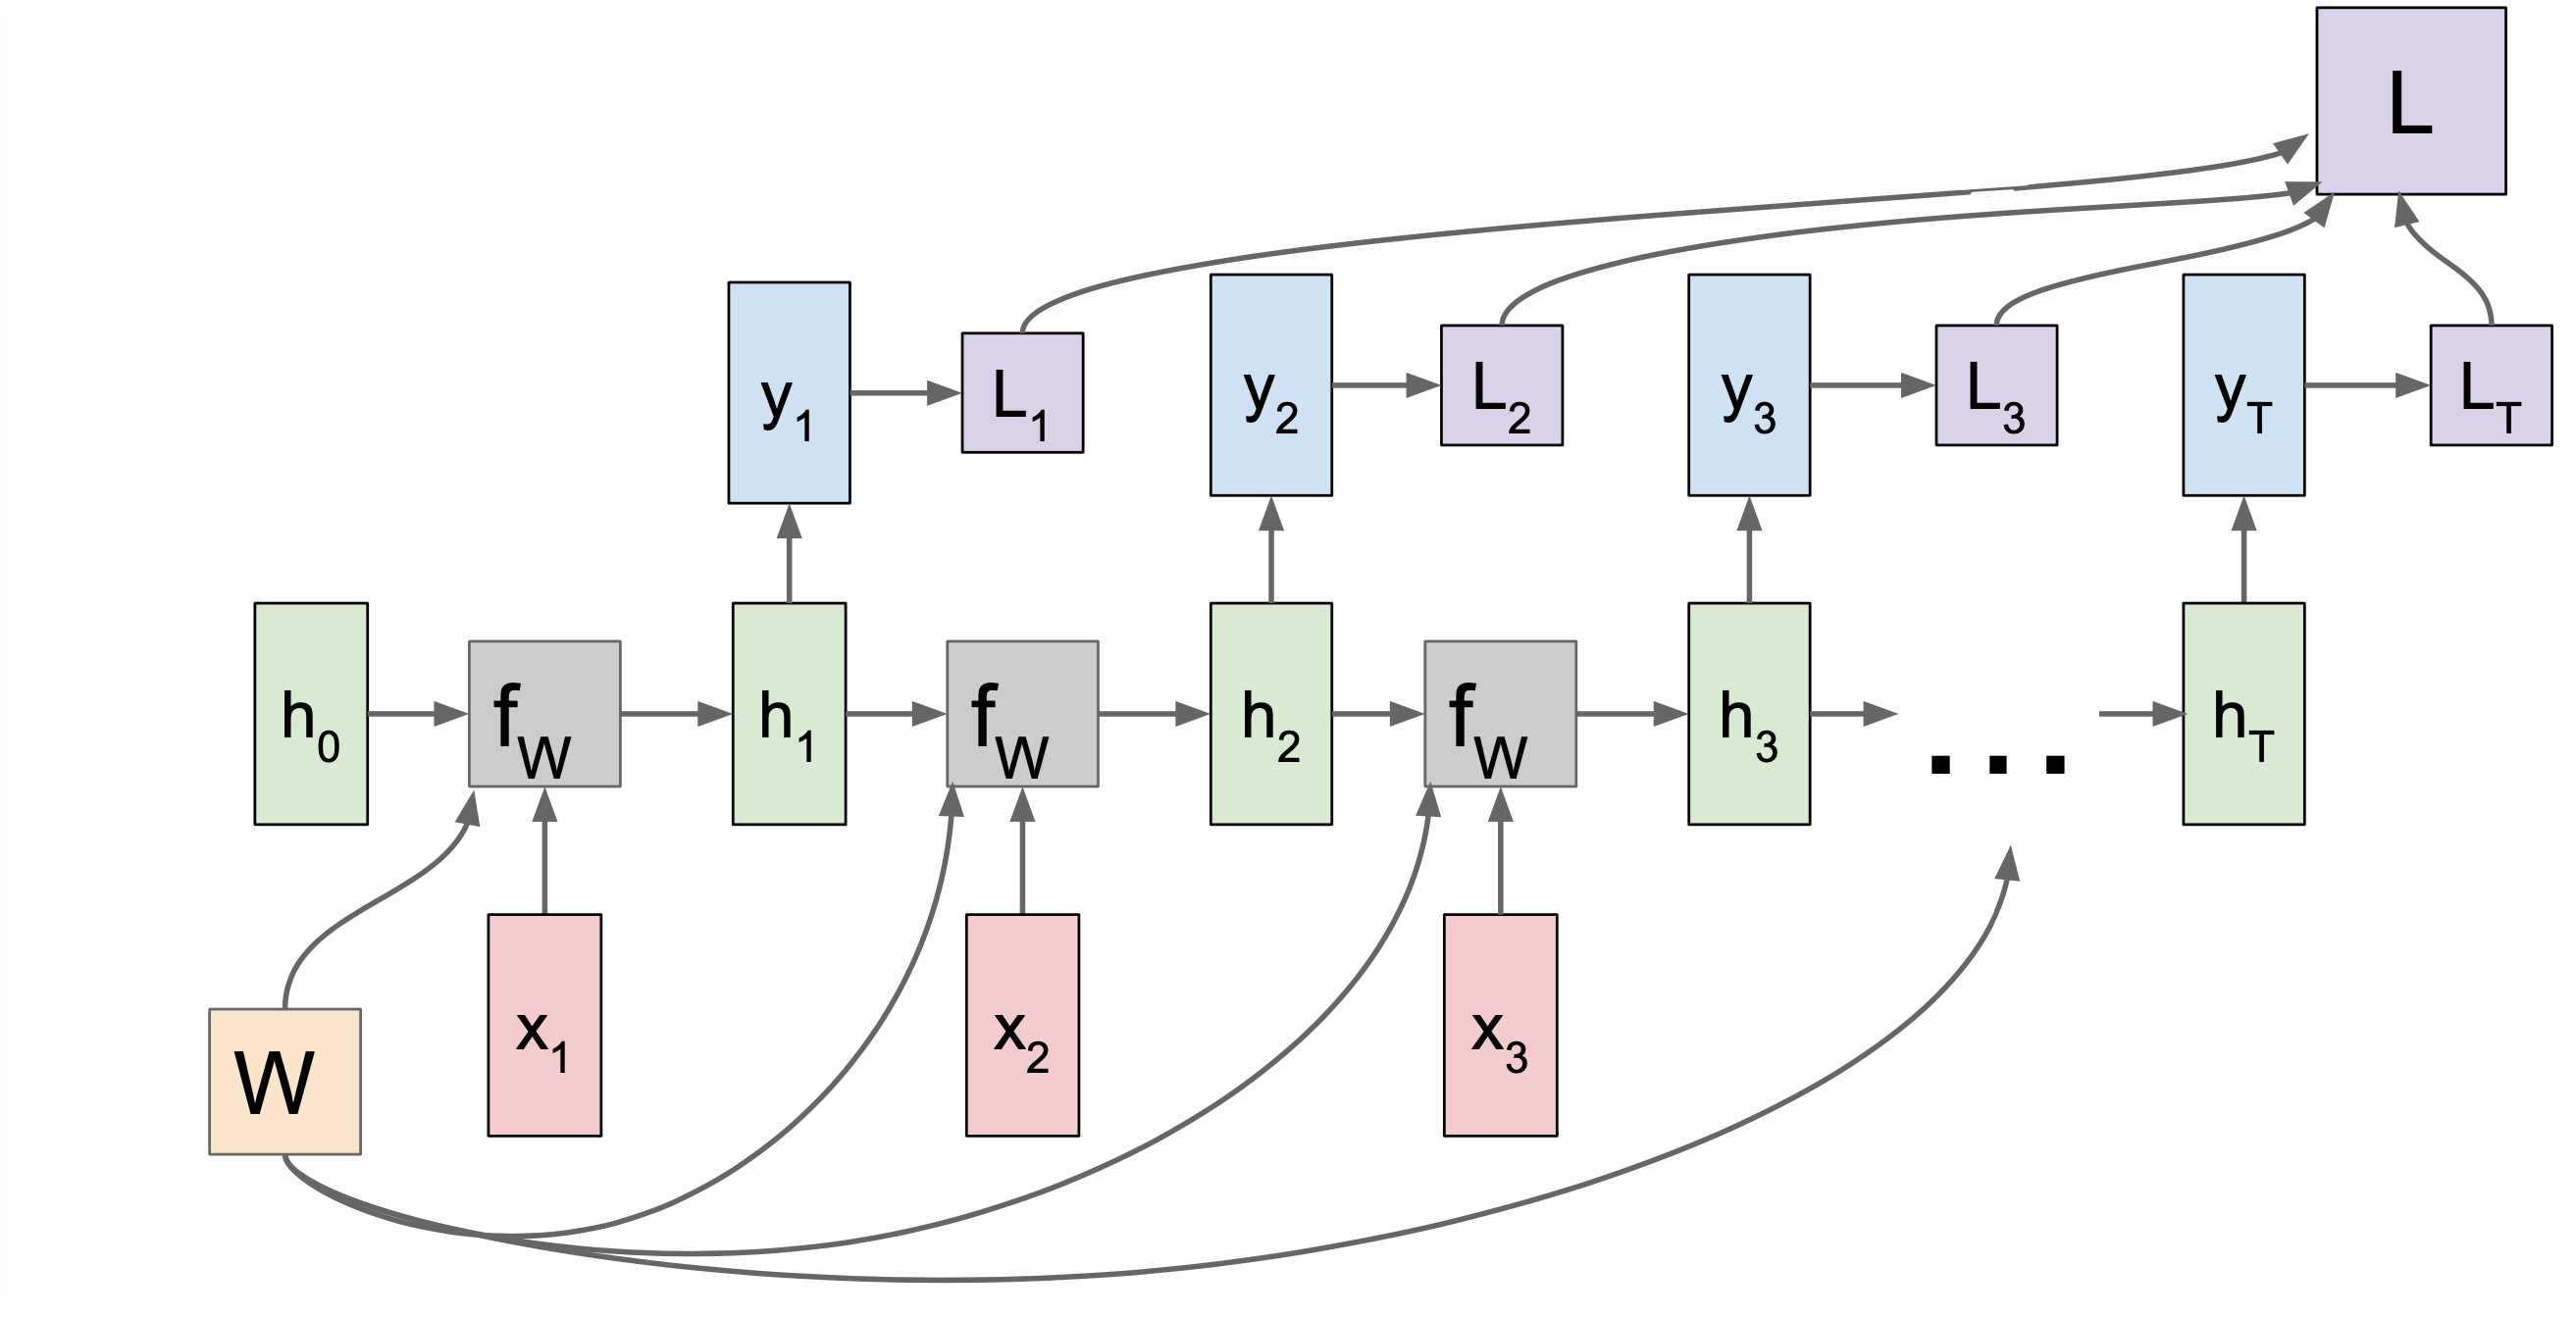
\includegraphics[width=.98\linewidth]{rnn-gr.png}
\end{center}
\vfill 
\footnotesize 
\color{blue} \url{http://cs231n.stanford.edu/schedule.html} 
\end{frame}


\begin{frame}{Backpropagation through time}
\begin{columns}
	\begin{column}{.48\linewidth}
		{\large
			\color{blue} Forward pass: \\ $\qquad h_t, \hat{y}_t, L_t, L$ \\ \vspace{1cm}
			\color{red} Backward pass: \\ $\qquad \frac{\partial L}{\partial U}, \frac{\partial L}{\partial V}, \frac{\partial L}{\partial W}$}
	
	\end{column}
	\begin{column}{.48\linewidth}
		\begin{center}
			\begin{tikzpicture}
			\tikzstyle{place}=[circle, draw=black, minimum size = 12mm]
			\tikzstyle{placeh}=[minimum height=32pt,minimum width=32pt, inner sep=2pt, draw=black]
			
			\node at (-1.2,0.08) (here) {};
			
			\draw node at (0, 2) [place, fill=blue, opacity=0.1] (y) {$\hat y_{t-2}$};
			\draw node at (0, 2) [place] {$\hat y_{t-2}$};  % мои костыли максимально всратые
			\draw node at (0, 0) [placeh, fill=red, opacity=0.1] (h) {$h_{t-2}$};
			\draw node at (0, 0) [placeh] {$h_{t-2}$};
			\draw node at (0, -2) [place, fill=green, opacity=0.1] (x) {$x_{t-2}$};
			\draw node at (0, -2) [place] {$x_{t-2}$};
			
			\draw [->]  (here) to (h);
			\draw [->]  (x) to node[left]{$V$} (h);
			\draw [->]  (h) to node[left]{$U$} (y);
			
			\draw node at (2, 2) [place, fill=blue, opacity=0.1] (y1) {$\hat y_{t-1}$};
			\draw node at (2, 2) [place] {$\hat y_{t-1}$};  % мои костыли максимально всратые
			\draw node at (2, 0) [placeh, fill=red, opacity=0.1] (h1) {$h_{t-1}$};
			\draw node at (2, 0) [placeh] {$h_{t-1}$};
			\draw node at (2, -2) [place, fill=green, opacity=0.1] (x1) {$x_{t-1}$};
			\draw node at (2, -2) [place] {$x_{t-1}$};
			
			\draw [->]  (h) to node[above]{$W$} (h1);
			\draw [->]  (x1) to node[left]{$V$} (h1);
			\draw [->]  (h1) to node[left]{$U$} (y1);
			
			\draw node at (4, 2) [place, fill=blue, opacity=0.1] (y2) {$\hat y_{t}$};
			\draw node at (4, 2) [place] {$\hat y_{t}$};  % мои костыли максимально всратые
			\draw node at (4, 0) [placeh, fill=red, opacity=0.1] (h2) {$h_{t}$};
			\draw node at (4, 0) [placeh] {$h_{t}$};
			\draw node at (4, -2) [place, fill=green, opacity=0.1] (x2) {$x_{t}$};
			\draw node at (4, -2) [place] {$x_{t}$};
			
			\draw [->]  (h1) to node[above]{$W$} (h2);
			\draw [->]  (x2) to node[left]{$V$} (h2);
			\draw [->]  (h2) to node[left]{$U$} (y2);
			
			\node at (5.2,0.08) (end) {};
			\draw [->]  (h2) to node[above]{$W$} (end);
			
			\draw node at (4, 3.5)  (l2){$L_{t}$}; 
			\draw node at (2, 3.5)  (l1){$L_{t-1}$};
			\draw node at (0, 3.5)  (l){$L_{t-2}$};
			\draw node at (2, 4.5)  (sl){$L$};
			\draw [->]  (y) to  (l);
			\draw [->]  (y1) to  (l1);
			\draw [->]  (y2) to  (l2);		
			\draw [->]  (l) to  (sl);	
			\draw [->]  (l1) to  (sl);	
			\draw [->]  (l2) to  (sl);
			
			\draw [->, red, line width=2.pt]   (5.2,-2.65)  to  (-1.2, -2.65);
			\draw [->, red, line width=2.pt]  (5.2, 4.2)  to  (5.2, -2);
			\end{tikzpicture}
		\end{center}
	\end{column}	
\end{columns}
\end{frame}


\begin{frame}{Backpropagation through time}
\begin{columns}
	\begin{column}{.48\linewidth}
		
		\only<1-4>{{\large
				\[\frac{\partial L}{\partial U} = \sum_{i=0}^T \frac{\partial L_i}{\partial U}\]
		}}			
		
		\only<2-3>{{\large
				\[\frac{\partial L_t}{\partial U} = \frac{\partial L_t}{\partial \hat{y}_t} \cdot \frac{\partial \hat{y}_t}{\partial U}\]
		}}	
	
		\only<4>{{\large
			\[\frac{\partial L_t}{\partial U} = \frac{\partial L_t}{\partial \hat{y}_t} \alert{\cdot f'_y(\ldots) \cdot h_t}\]
		}}	
		
		\only<3-4>{{\large
						\begin{equation*} 
				\begin{aligned}
				h_t =& f_h(b_h +W \cdot h_{t-1} + V \cdot x_t)\\
				\hat{y}_t =& f_y(b_y + \alert{U} \cdot h_t)
				\end{aligned}
				\end{equation*} 
		}}	
		\only<3>{\alert{Параметр $U$ в одном месте!}}
		
	\end{column}
	\begin{column}{.48\linewidth}
		\begin{center}
			\begin{tikzpicture}
			\tikzstyle{place}=[circle, draw=black, minimum size = 12mm]
			\tikzstyle{placeh}=[minimum height=32pt,minimum width=32pt, inner sep=2pt, draw=black]
			
			\node at (-1.2,0.08) (here) {};
			
			\draw node at (0, 2) [place, fill=blue, opacity=0.1] (y) {$\hat y_{t-2}$};
			\draw node at (0, 2) [place] {$\hat y_{t-2}$};  % мои костыли максимально всратые
			\draw node at (0, 0) [placeh, fill=red, opacity=0.1] (h) {$h_{t-2}$};
			\draw node at (0, 0) [placeh] {$h_{t-2}$};
			\draw node at (0, -2) [place, fill=green, opacity=0.1] (x) {$x_{t-2}$};
			\draw node at (0, -2) [place] {$x_{t-2}$};
			
			\draw [->]  (here) to (h);
			\draw [->]  (x) to node[left]{} (h);
			\draw [->]  (h) to node[left]{$U$} (y);
			
			\draw node at (2, 2) [place, fill=blue, opacity=0.1] (y1) {$\hat y_{t-1}$};
			\draw node at (2, 2) [place] {$\hat y_{t-1}$};  % мои костыли максимально всратые
			\draw node at (2, 0) [placeh, fill=red, opacity=0.1] (h1) {$h_{t-1}$};
			\draw node at (2, 0) [placeh] {$h_{t-1}$};
			\draw node at (2, -2) [place, fill=green, opacity=0.1] (x1) {$x_{t-1}$};
			\draw node at (2, -2) [place] {$x_{t-1}$};
			
			\draw [->]  (h) to node[above]{} (h1);
			\draw [->]  (x1) to node[left]{} (h1);
			\draw [->]  (h1) to node[left]{$U$} (y1);
			
			\draw node at (4, 2) [place, fill=blue, opacity=0.1] (y2) {$\hat y_{t}$};
			\draw node at (4, 2) [place] {$\hat y_{t}$};  % мои костыли максимально всратые
			\draw node at (4, 0) [placeh, fill=red, opacity=0.1] (h2) {$h_{t}$};
			\draw node at (4, 0) [placeh] {$h_{t}$};
			\draw node at (4, -2) [place, fill=green, opacity=0.1] (x2) {$x_{t}$};
			\draw node at (4, -2) [place] {$x_{t}$};
			
			\draw [->]  (h1) to node[above]{} (h2);
			\draw [->]  (x2) to node[left]{} (h2);
			\draw [->]  (h2) to node[left]{$U$} (y2);
			
			\node at (5.2,0.08) (end) {};
			\draw [->]  (h2) to node[above]{} (end);
			
			\draw node at (4, 3.5)  (l2){$L_{t}$}; 
			\draw node at (2, 3.5)  (l1){$L_{t-1}$};
			\draw node at (0, 3.5)  (l){$L_{t-2}$};
			\draw node at (2, 4.5)  (sl){$L$};
			\draw [->]  (y) to  (l);
			\draw [->]  (y1) to  (l1);
			\draw [->]  (y2) to  (l2);		
			\draw [->]  (l) to  (sl);	
			\draw [->]  (l1) to  (sl);	
			\draw [->]  (l2) to  (sl);
			
			\only<1-4>{ 
				\draw [->, red, line width=2.pt]  (sl) to  (l);	
				\draw [->, red, line width=2.pt]  (sl) to  (l1);	
				\draw [->, red, line width=2.pt]  (sl) to  (l2);
			};
		
			\only<2-4>{ 
				\draw [->, red, line width=2.pt]  (l2) to  (y2);	
			};
		
			\only<3-4>{ 
				\draw [->, red, line width=2.pt]  (y2) to  (h2);	
			};
			
			\end{tikzpicture}
		\end{center}
	\end{column}	
\end{columns}
\end{frame}


\begin{frame}{Backpropagation through time}
\begin{columns}
	\begin{column}{.48\linewidth}
		
		\only<1-2>{{\large
				\[\frac{\partial L}{\partial W} = \sum_{i=0}^T \frac{\partial L_i}{\partial W}\]
				
				\[\frac{\partial L_t}{\partial W} = \frac{\partial L_t}{\partial \hat{y}_t} \cdot \frac{\partial \hat{y}_t}{\partial h_t} \cdot \alert{\frac{\partial h_t}{\partial W}} \]
				
				\begin{equation*} 
					\begin{aligned}
						 h_t =& f_h(b_h + \alert{W \cdot h_{t-1} }+ V \cdot x_t)\\
						\hat{y}_t =& f_y(b_y + U \cdot h_t)
					\end{aligned}
				\end{equation*} 
		}}	
	\only<1>{\alert{$W$ фигурирует в нескольких местах!}}
	\only<2>{{\large 
			\[\alert{\frac{\partial h_t}{\partial W} - ???} \]	
		}}
		
		
	\end{column}
	\begin{column}{.48\linewidth}
		\begin{center}
			\begin{tikzpicture}
			\tikzstyle{place}=[circle, draw=black, minimum size = 12mm]
			\tikzstyle{placeh}=[minimum height=32pt,minimum width=32pt, inner sep=2pt, draw=black]
			
			\node at (-1.2,0.08) (here) {};
			
			\draw node at (0, 2) [place, fill=blue, opacity=0.1] (y) {$\hat y_{t-2}$};
			\draw node at (0, 2) [place] {$\hat y_{t-2}$};  % мои костыли максимально всратые
			\draw node at (0, 0) [placeh, fill=red, opacity=0.1] (h) {$h_{t-2}$};
			\draw node at (0, 0) [placeh] {$h_{t-2}$};
			\draw node at (0, -2) [place, fill=green, opacity=0.1] (x) {$x_{t-2}$};
			\draw node at (0, -2) [place] {$x_{t-2}$};
			
			\draw [->]  (here) to (h);
			\draw [->]  (x) to node[left]{} (h);
			\draw [->]  (h) to node[left]{} (y);
			
			\draw node at (2, 2) [place, fill=blue, opacity=0.1] (y1) {$\hat y_{t-1}$};
			\draw node at (2, 2) [place] {$\hat y_{t-1}$};  % мои костыли максимально всратые
			\draw node at (2, 0) [placeh, fill=red, opacity=0.1] (h1) {$h_{t-1}$};
			\draw node at (2, 0) [placeh] {$h_{t-1}$};
			\draw node at (2, -2) [place, fill=green, opacity=0.1] (x1) {$x_{t-1}$};
			\draw node at (2, -2) [place] {$x_{t-1}$};
			
			\draw [->]  (h) to node[above]{$W$} (h1);
			\draw [->]  (x1) to node[left]{} (h1);
			\draw [->]  (h1) to node[left]{} (y1);
			
			\draw node at (4, 2) [place, fill=blue, opacity=0.1] (y2) {$\hat y_{t}$};
			\draw node at (4, 2) [place] {$\hat y_{t}$};  % мои костыли максимально всратые
			\draw node at (4, 0) [placeh, fill=red, opacity=0.1] (h2) {$h_{t}$};
			\draw node at (4, 0) [placeh] {$h_{t}$};
			\draw node at (4, -2) [place, fill=green, opacity=0.1] (x2) {$x_{t}$};
			\draw node at (4, -2) [place] {$x_{t}$};
			
			\draw [->]  (h1) to node[above]{$W$} (h2);
			\draw [->]  (x2) to node[left]{} (h2);
			\draw [->]  (h2) to node[left]{} (y2);
			
			\node at (5.2,0.08) (end) {};
			\draw [->]  (h2) to node[above]{$W$} (end);
			
			\draw node at (4, 3.5)  (l2){$L_{t}$}; 
			\draw node at (2, 3.5)  (l1){$L_{t-1}$};
			\draw node at (0, 3.5)  (l){$L_{t-2}$};
			\draw node at (2, 4.5)  (sl){$L$};
			\draw [->]  (y) to  (l);
			\draw [->]  (y1) to  (l1);
			\draw [->]  (y2) to  (l2);		
			\draw [->]  (l) to  (sl);	
			\draw [->]  (l1) to  (sl);	
			\draw [->]  (l2) to  (sl);
			
			\only<1-2>{ 
				\draw [->, red, line width=2.pt]  (sl) to  (l);	
				\draw [->, red, line width=2.pt]  (sl) to  (l1);	
				\draw [->, red, line width=2.pt]  (sl) to  (l2);
				\draw [->, red, line width=2.pt]  (l2) to  (y2);	
				\draw [->, red, line width=2.pt]  (y2) to  (h2);	
			};
		
			\only<2>{ 
				\draw [->, red, line width=2.pt]  (h2) to  (h1);	
				\draw [->, red, line width=2.pt]  (h1) to  (h);
				\draw [->, red, line width=2.pt]  (h) to  (here);		
			};
			\end{tikzpicture}
		\end{center}
	\end{column}	
\end{columns}
\end{frame}


\begin{frame}
\begin{center}
	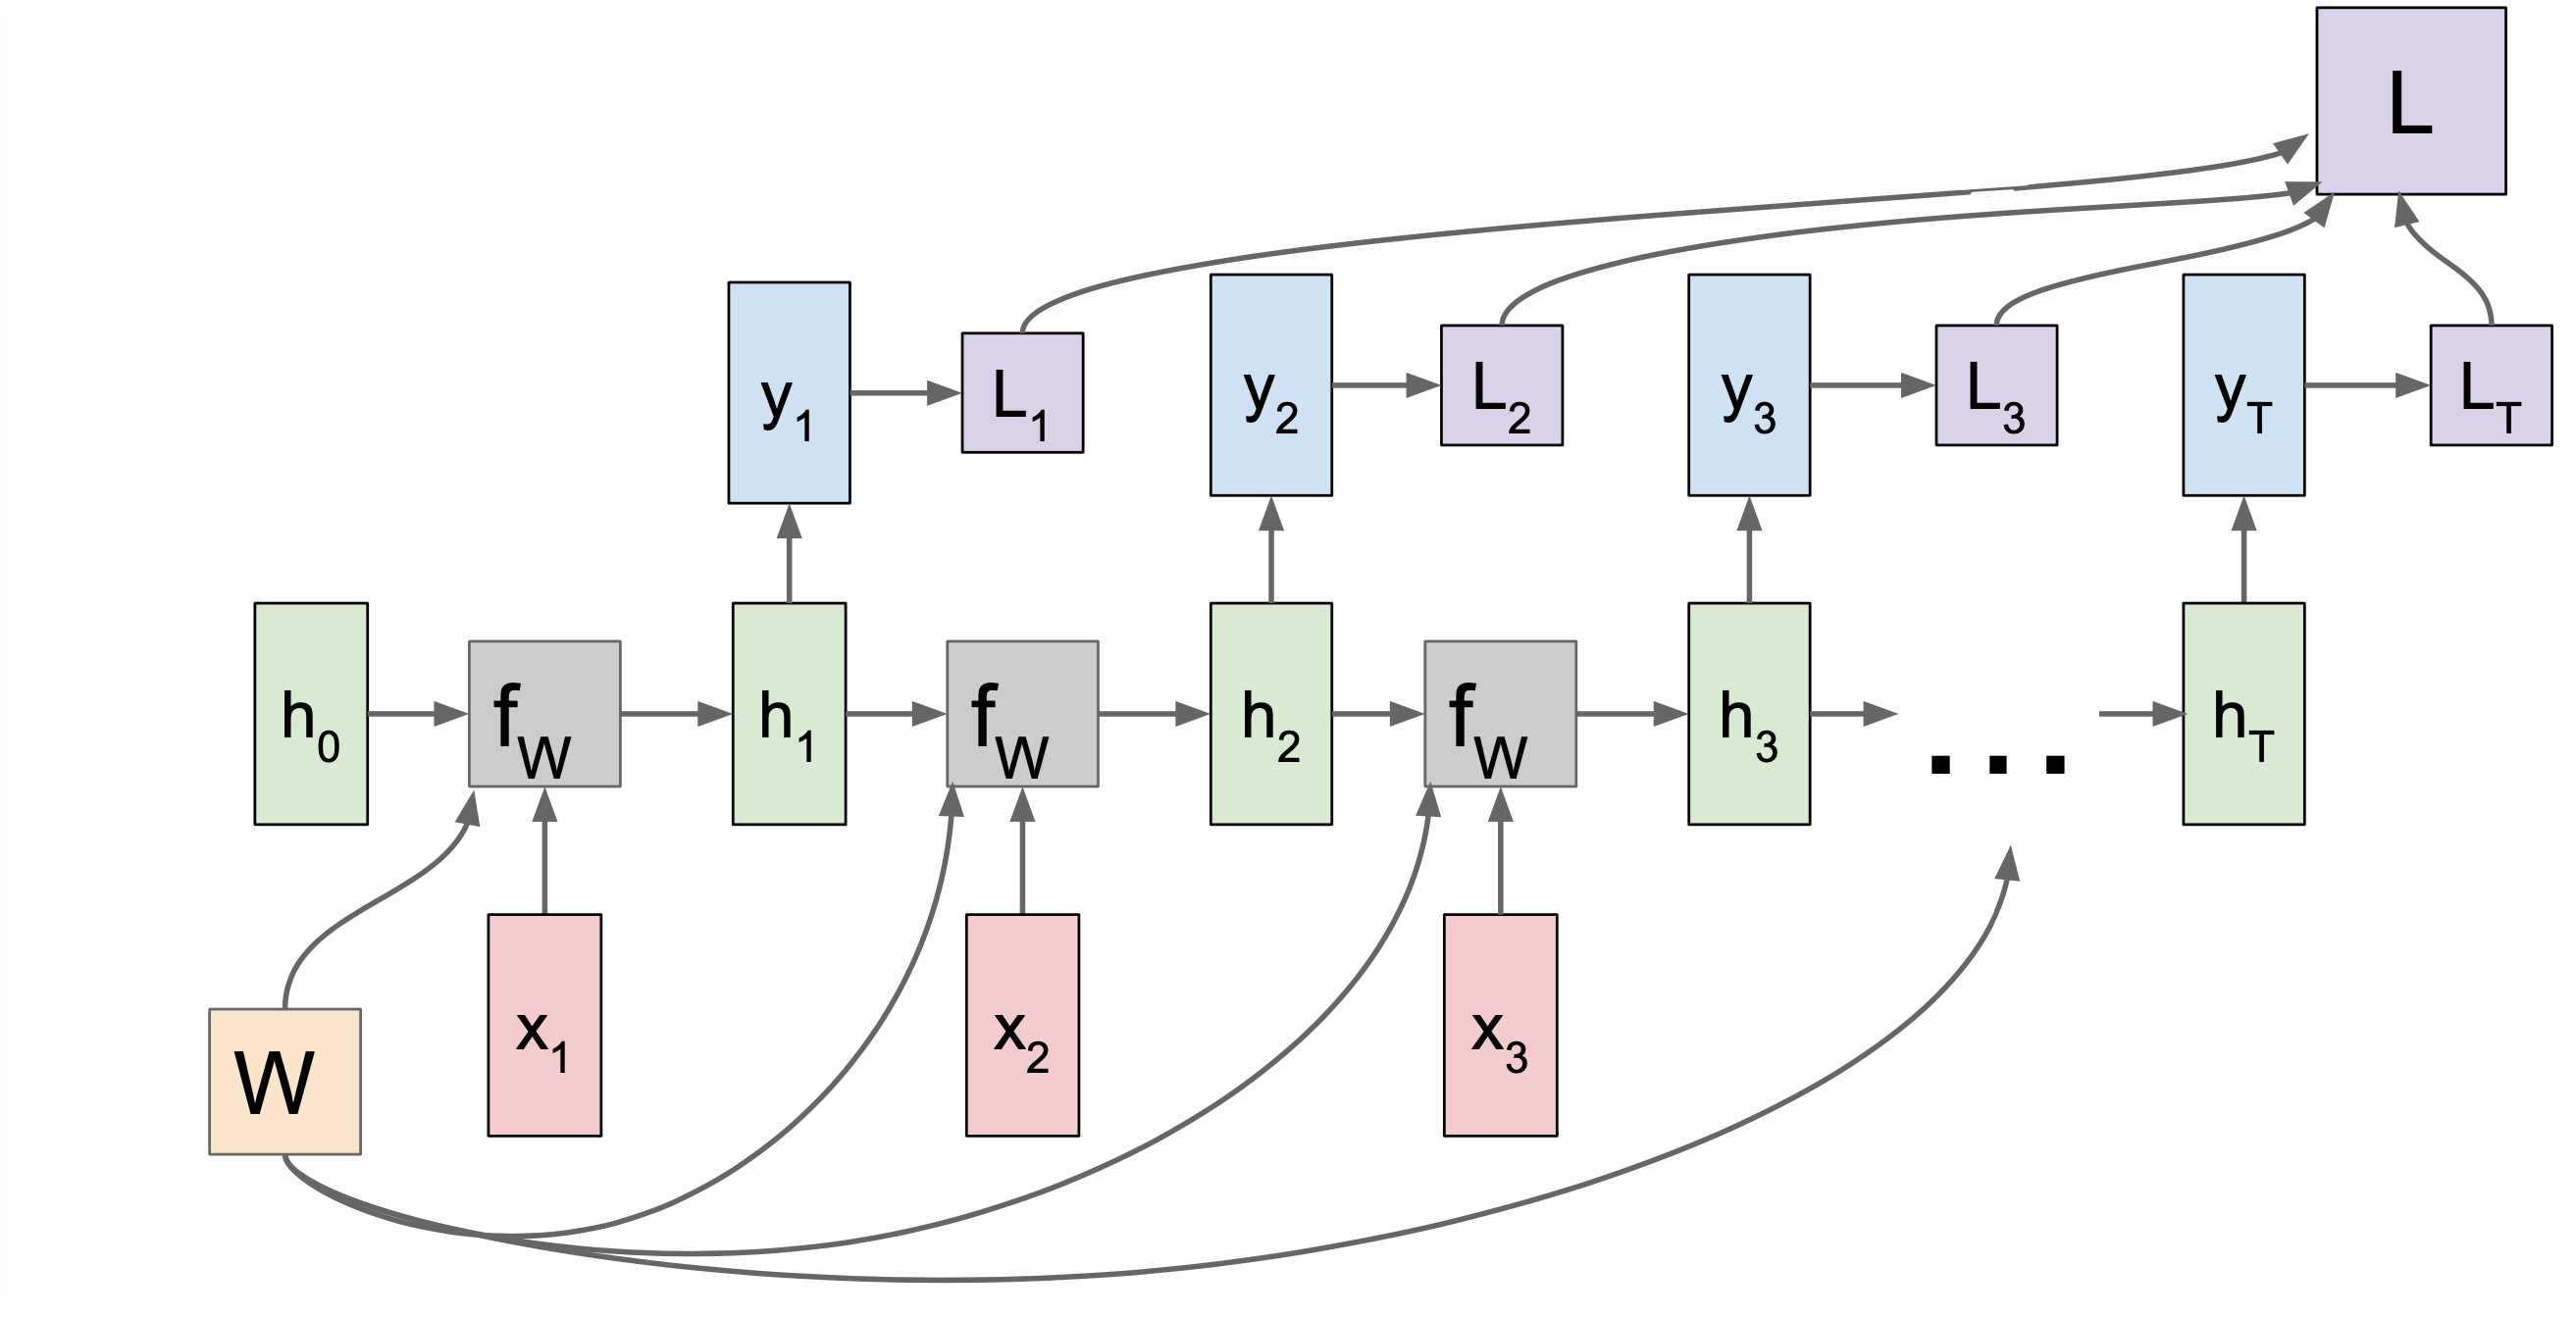
\includegraphics[width=.98\linewidth]{rnn-gr.png}
\end{center}
\vfill 
\footnotesize 
\color{blue} \url{http://cs231n.stanford.edu/schedule.html} 
\end{frame}


\begin{frame}{Backpropagation through time}
\begin{columns}
	\begin{column}{.48\linewidth}
		
		{\large
				
				\[\frac{\partial L_t}{\partial W} = \frac{\partial L_t}{\partial \hat{y}_t} \cdot \frac{\partial \hat{y}_t}{\partial h_t} \cdot \frac{\partial h_t}{\partial W} \]
				
				\begin{equation*} 
					\begin{aligned}
						h_t =& f_h(b_h + W \cdot h_{t-1} + V \cdot x_t)\\
						\hat{y}_t =& f_y(b_y + U \cdot h_t)
					\end{aligned}
				\end{equation*} 

				\[\frac{\partial h_t}{\partial W} =  \frac{\partial h_t}{\partial W}  + \frac{\partial h_t}{\partial h_{t-1}} \cdot \frac{\partial h_{t-1}}{\partial W}   + \ldots  \]	
		}
		
	\end{column}
	\begin{column}{.48\linewidth}
		\begin{center}
			\begin{tikzpicture}
			\tikzstyle{place}=[circle, draw=black, minimum size = 12mm]
			\tikzstyle{placeh}=[minimum height=32pt,minimum width=32pt, inner sep=2pt, draw=black]
			
			\node at (-1.2,0.08) (here) {};
			
			\draw node at (0, 2) [place, fill=blue, opacity=0.1] (y) {$\hat y_{t-2}$};
			\draw node at (0, 2) [place] {$\hat y_{t-2}$};  % мои костыли максимально всратые
			\draw node at (0, 0) [placeh, fill=red, opacity=0.1] (h) {$h_{t-2}$};
			\draw node at (0, 0) [placeh] {$h_{t-2}$};
			\draw node at (0, -2) [place, fill=green, opacity=0.1] (x) {$x_{t-2}$};
			\draw node at (0, -2) [place] {$x_{t-2}$};
			
			\draw [->]  (here) to (h);
			\draw [->]  (x) to node[left]{} (h);
			\draw [->]  (h) to node[left]{} (y);
			
			\draw node at (2, 2) [place, fill=blue, opacity=0.1] (y1) {$\hat y_{t-1}$};
			\draw node at (2, 2) [place] {$\hat y_{t-1}$};  % мои костыли максимально всратые
			\draw node at (2, 0) [placeh, fill=red, opacity=0.1] (h1) {$h_{t-1}$};
			\draw node at (2, 0) [placeh] {$h_{t-1}$};
			\draw node at (2, -2) [place, fill=green, opacity=0.1] (x1) {$x_{t-1}$};
			\draw node at (2, -2) [place] {$x_{t-1}$};
			
			\draw [->]  (h) to node[above]{$W$} (h1);
			\draw [->]  (x1) to node[left]{} (h1);
			\draw [->]  (h1) to node[left]{} (y1);
			
			\draw node at (4, 2) [place, fill=blue, opacity=0.1] (y2) {$\hat y_{t}$};
			\draw node at (4, 2) [place] {$\hat y_{t}$};  % мои костыли максимально всратые
			\draw node at (4, 0) [placeh, fill=red, opacity=0.1] (h2) {$h_{t}$};
			\draw node at (4, 0) [placeh] {$h_{t}$};
			\draw node at (4, -2) [place, fill=green, opacity=0.1] (x2) {$x_{t}$};
			\draw node at (4, -2) [place] {$x_{t}$};
			
			\draw [->]  (h1) to node[above]{$W$} (h2);
			\draw [->]  (x2) to node[left]{} (h2);
			\draw [->]  (h2) to node[left]{} (y2);
			
			\node at (5.2,0.08) (end) {};
			\draw [->]  (h2) to node[above]{$W$} (end);
			
			\draw node at (4, 3.5)  (l2){$L_{t}$}; 
			\draw node at (2, 3.5)  (l1){$L_{t-1}$};
			\draw node at (0, 3.5)  (l){$L_{t-2}$};
			\draw node at (2, 4.5)  (sl){$L$};
			\draw [->]  (y) to  (l);
			\draw [->]  (y1) to  (l1);
			\draw [->]  (y2) to  (l2);		
			\draw [->]  (l) to  (sl);	
			\draw [->]  (l1) to  (sl);	
			\draw [->]  (l2) to  (sl);
			
				\draw [->, red, line width=2.pt]  (sl) to  (l);	
				\draw [->, red, line width=2.pt]  (sl) to  (l1);	
				\draw [->, red, line width=2.pt]  (sl) to  (l2);
				\draw [->, red, line width=2.pt]  (l2) to  (y2);	
				\draw [->, red, line width=2.pt]  (y2) to  (h2);	
				\draw [->, red, line width=2.pt]  (h2) to  (h1);	
				\draw [->, red, line width=2.pt]  (h1) to  (h);
				\draw [->, red, line width=2.pt]  (h) to  (here);		
			\end{tikzpicture}
		\end{center}
	\end{column}	
\end{columns}
\end{frame}


\begin{frame}{Vanishing and Exploding}
	\large
			
	\[\frac{\partial L_t}{\partial W}  \propto \sum_{k=0}^t \left( \alert{\prod_{i=k+1}^t  \frac{\partial h_i}{\partial h_{i-1}}} \right) \cdot  \frac{\partial h_k}{\partial W} \]
					
	\begin{equation*} 
			\begin{aligned}
					&\left\|  \frac{\partial h_i}{\partial h_{i-1}} \right\|_2 < 1 \qquad \Rightarrow  \qquad  \text{Затухание градиентов} \\
					&\left\|  \frac{\partial h_i}{\partial h_{i-1}} \right\|_2 > 1 \qquad \Rightarrow   \qquad  \text{Взрыв градиентов}
			\end{aligned}
	\end{equation*} 
\end{frame}


\begin{frame}{Как понять, что градиент взорвался?}
\begin{center}
	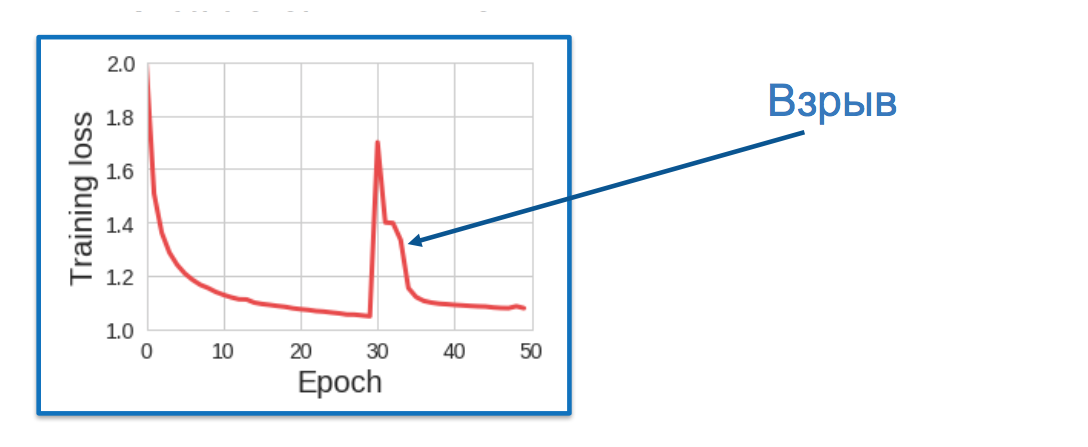
\includegraphics[width=.9\linewidth]{rnn9.png}
\end{center}
Что делать со взрывом? \only<2>{ \alert{$\Rightarrow $ ограничить градиент }}
\end{frame}


\begin{frame}{Ограничение градиентов (Gradient clipping)}

Если  

\[
g = \frac{\partial L}{\partial w},  \qquad \left\| g \right\|_2 > treshold 
\]

тогда 

\[
g = \frac{treshold}{\|g\|} \cdot g
\]

\alert{Приём простой и работает :)}

\vfill 
\footnotesize 
\color{blue} \url{https://arxiv.org/abs/1211.5063} 
\end{frame}


\begin{frame}{Урезанное обучение}
\begin{center}
	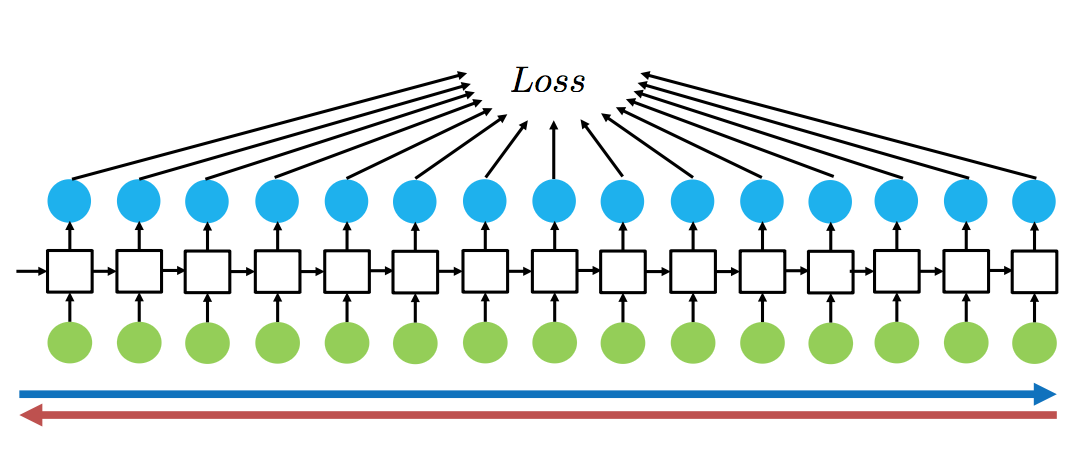
\includegraphics[width=.9\linewidth]{rnn10.png}
\end{center}
\end{frame}


\begin{frame}{Урезанное обучение}
\begin{center}
	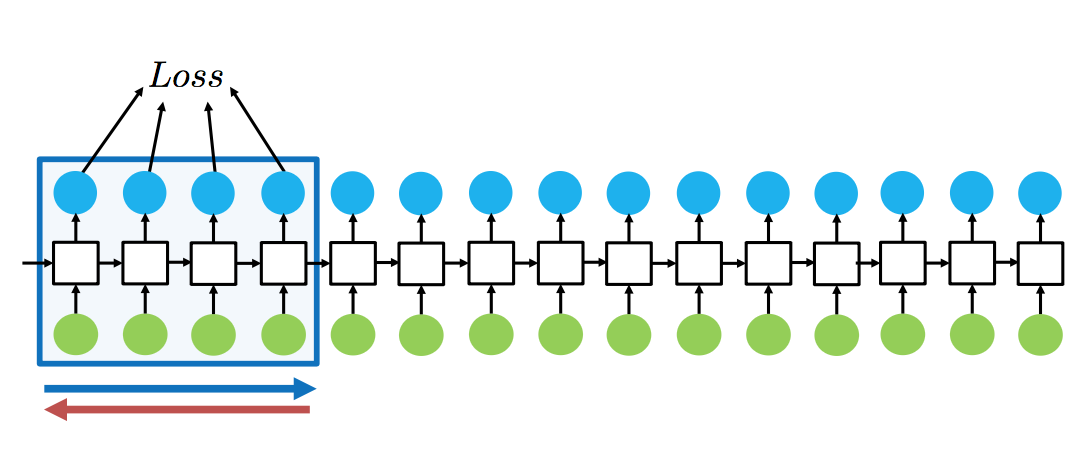
\includegraphics[width=.9\linewidth]{rnn11.png}
\end{center}
\end{frame}


\begin{frame}{Урезанное обучение}
\begin{center}
	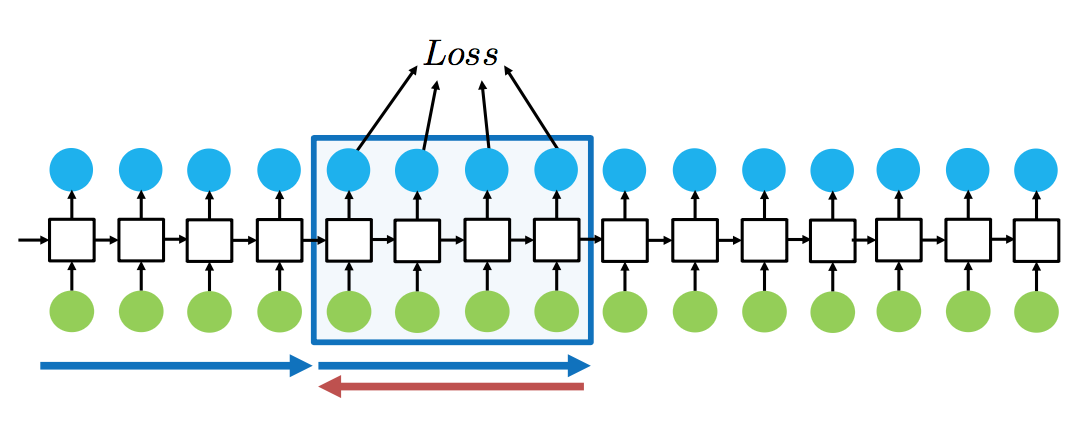
\includegraphics[width=.9\linewidth]{rnn12.png}
\end{center}
\end{frame}


\begin{frame}{Как предотвратить взрыв?}
	\begin{wideitemize} 
		\item Урезанное обучение работает быстрее обычного
		\item Однако у него есть своя цена
		\item Сетка не выучит зависимости, которые превышают размер блока 
	\end{wideitemize} 
\end{frame}


\begin{frame}{Как понять, что градиент затухает?}
\begin{center}
	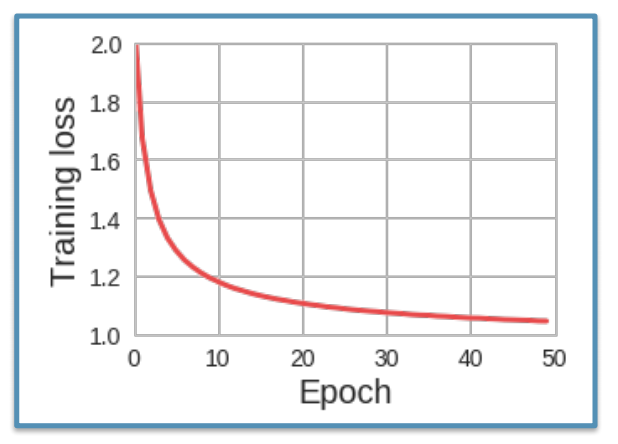
\includegraphics[width=.5\linewidth]{rnn9_1.png}
\end{center}
Толи обучение сошлось, толи градиенты очень маленькие. Нельзя понять, что градиент затухает, не поправив это и не получив улучшение качества. 
\end{frame}

\begin{frame}{Как предотвратить затухание градиентов?}
\begin{wideitemize} 
	\item Аккуратная инициализация 
	\item Skip connections
	\item Модели с гейтами: LSTM, GRU
	\item Регуляризация
	\item \ldots 
\end{wideitemize} 
\end{frame}


\begin{frame}{Изучим градиенты подробнее}
	\large
		\begin{equation*} 
			\begin{aligned}
				h_t =& f_h(b_h + W \cdot h_{t-1} + V \cdot x_t) = f_h(pr_t)\\
				\hat{y}_t =& f_y(b_y + U \cdot h_t)
			\end{aligned}
		\end{equation*} 
		
		\par \mbox{} \par
		
		\[\frac{\partial L_t}{\partial W}  \propto \sum_{k=0}^t \left( \alert{\prod_{i=k+1}^t  \frac{\partial h_i}{\partial h_{i-1}}} \right) \cdot  \frac{\partial h_k}{\partial W} \]
		
		\par \mbox{} \par
		
	\only<2>{
		\[
			\frac{\partial h_i}{\partial h_{i-1}} = \frac{\partial h_i}{\partial inp_i} \cdot \frac{\partial inp_i}{\partial h_{i-1}} = diag(f'_h(pr_t)) \cdot \alert{?}
		\]
	}		

		\par \mbox{} \par
		
	\only<3>{
		\[
			\frac{\partial h_i}{\partial h_{i-1}} = \frac{\partial h_i}{\partial inp_i} \cdot \frac{\partial inp_i}{\partial h_{i-1}} = diag(f'_h(pr_t)) \cdot \alert{W}
		\]
	}	
\end{frame}



\begin{frame}{Аккуратная инициализация (2015)}
		
		\[\frac{\partial L_t}{\partial W}  \propto \sum_{k=0}^t \left( \alert{\prod_{i=k+1}^t  \frac{\partial h_i}{\partial h_{i-1}}} \right) \cdot  \frac{\partial h_k}{\partial W} \]
				
		\[
		\frac{\partial h_i}{\partial h_{i-1}} = \frac{\partial h_i}{\partial inp_i} \cdot \frac{\partial inp_i}{\partial h_{i-1}} = diag(f'_h(pr_t)) \cdot W
		\]
	
	\begin{wideitemize} 
		\item Функция активации $f_h(pr_t)$ не должна способствовать затуханию градиентов
		
		\item Если $W$ ортогональная матрица, тогда $W^T W = I, \quad W^{-1} = W^T$ и  произведение $\prod_i W_i$ не будет взрываться и затухать % (все собственные числа либо 0 либо 1)
	
		\item Инициализируем $W$ ортогональной матрицей
	\end{wideitemize} 
	
	\vfill 
	\footnotesize 
	\color{blue} \url{https://arxiv.org/abs/1504.00941} 
\end{frame}


\begin{frame}{Skip-connection}
	\begin{center}
		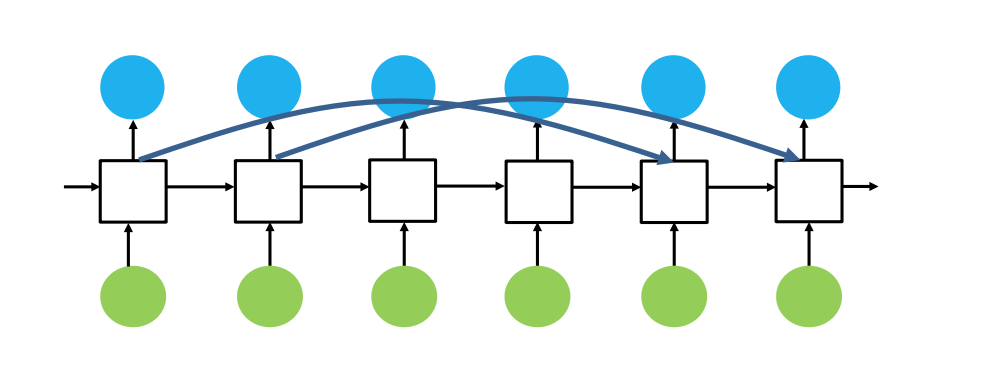
\includegraphics[width=.9\linewidth]{rnn13.png}
	\end{center}

	\begin{wideitemize} 
	\item  Более короткие маршруты для градиентов позволяют избежать затухания, похожая идея использовалась в ResNet
	\end{wideitemize} 
\end{frame}



\begin{transitionframe}
	\begin{center}
		\Huge LSTM (long short-term memory)
	\end{center}
%\centering 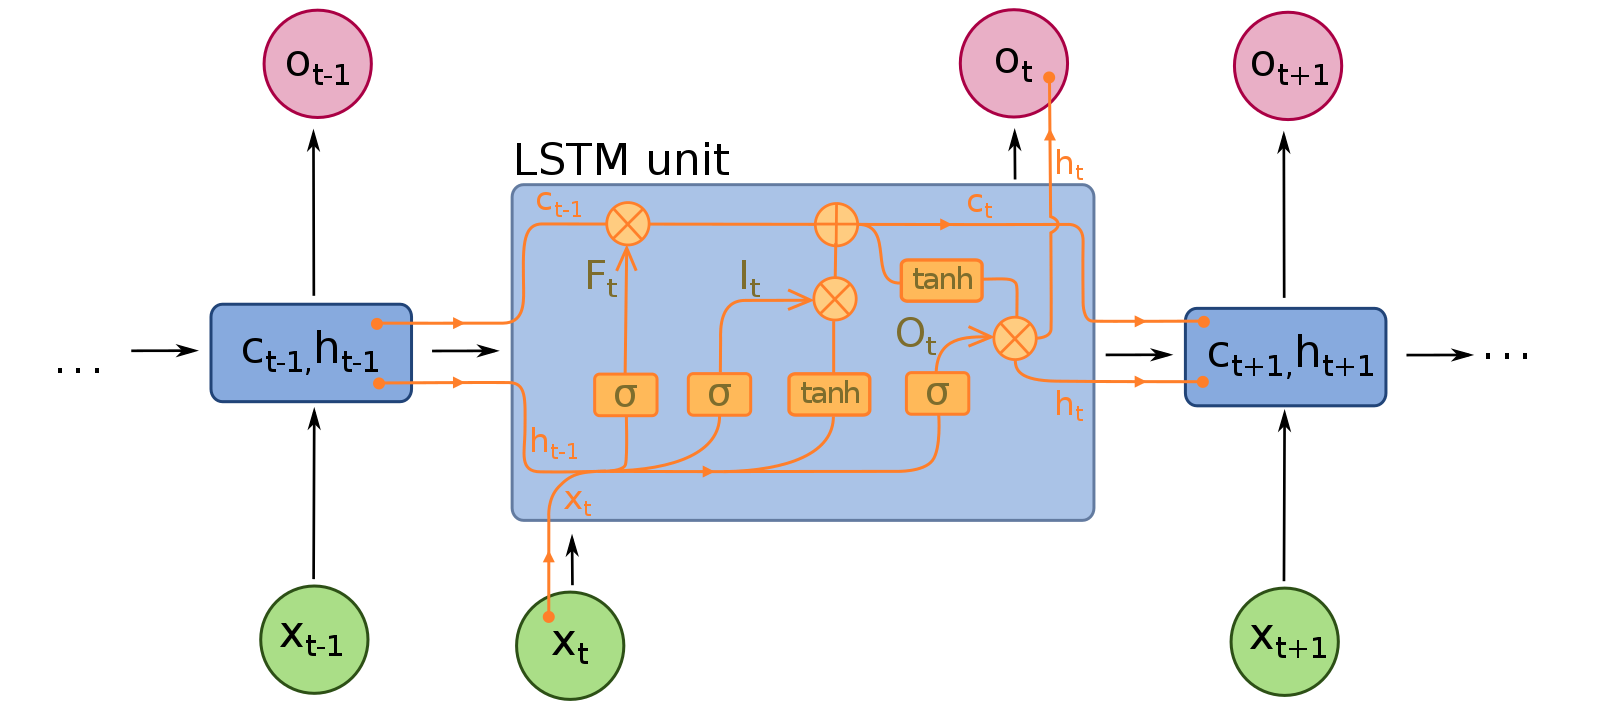
\includegraphics[scale = 0.15]{lstm-start.png}
\centering 
\includegraphics[scale = 0.35]{lstm_fish.jpg}
\end{transitionframe}


\begin{frame}{Короткая память}
\begin{wideitemize}
	\item  Привлекательность RNN в том, что они потенциально умеют связывать предыдущую информацию с текущей
	
	\item При backpropagation текущие градиенты пробрасываются во времени назад
	
	\item  Если градиент не взрывается, он постепенно затухает, получается что влияние текущего слоя не может проброситься во времени слишком далеко назад 
	
	\item Влияние текущего слоя затухает экспоненциально по мере удаления и мешает обычным RNN находить в данных "далёкие" зависимости
\end{wideitemize}
\end{frame}


\begin{frame}{Короткая память}
\begin{center}
	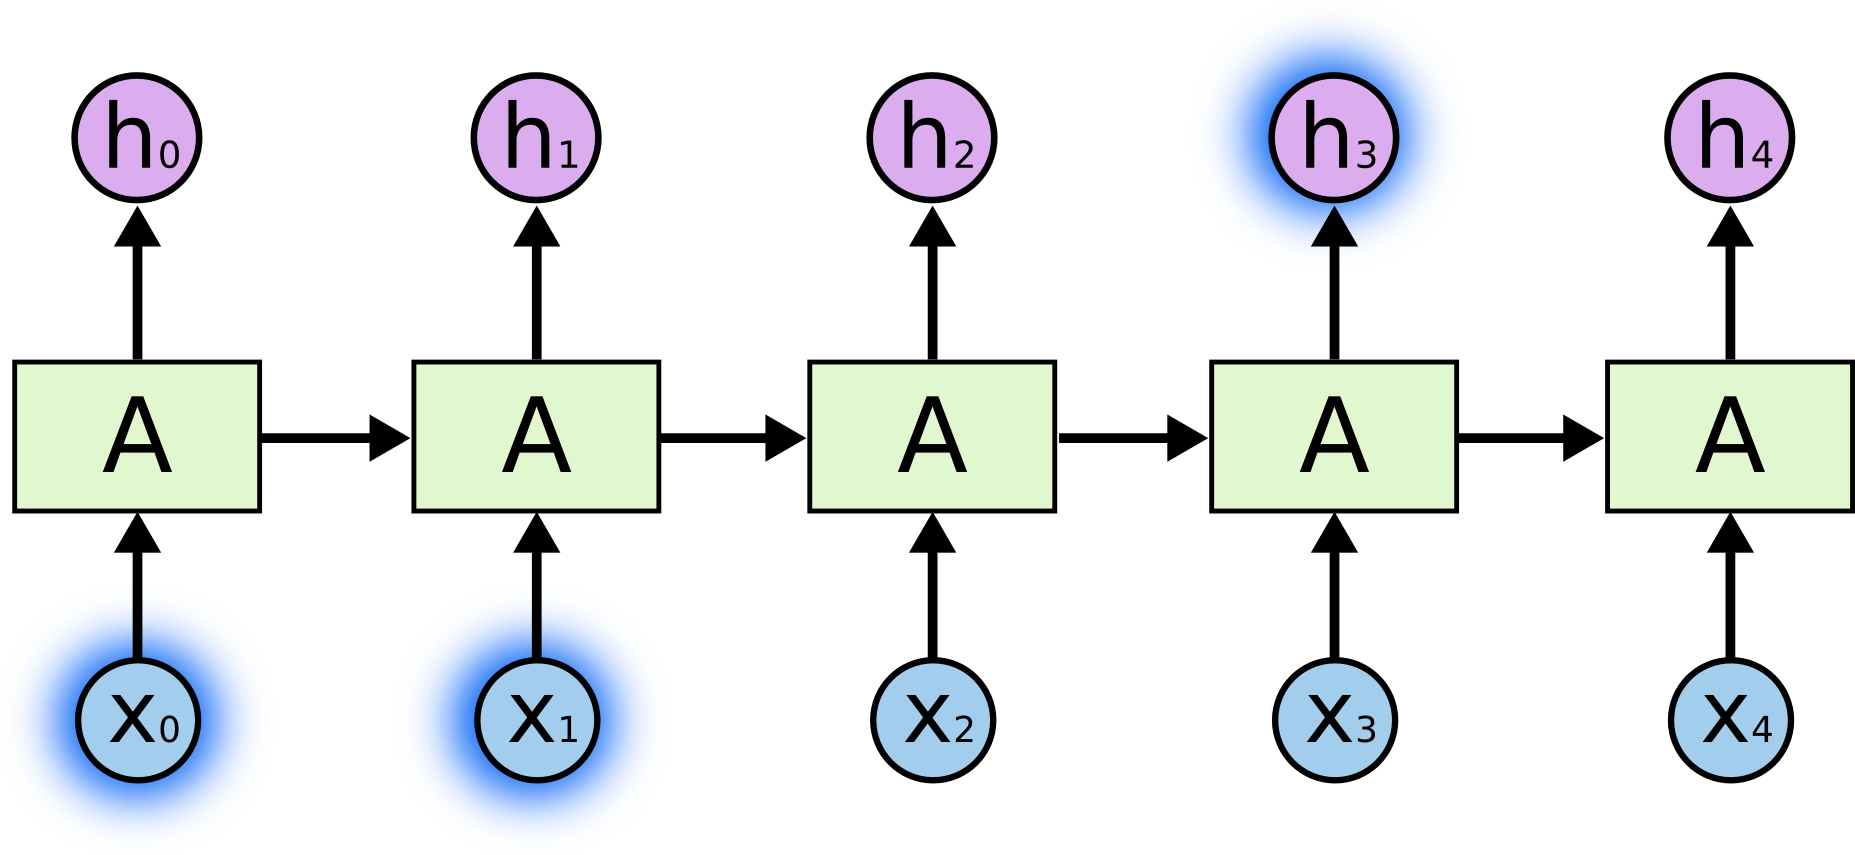
\includegraphics[width=.7\linewidth]{simple_rnn1.png}
\end{center}

\large Облака плывут по небу 
\end{frame}


\begin{frame}{Короткая память}
\begin{center}
	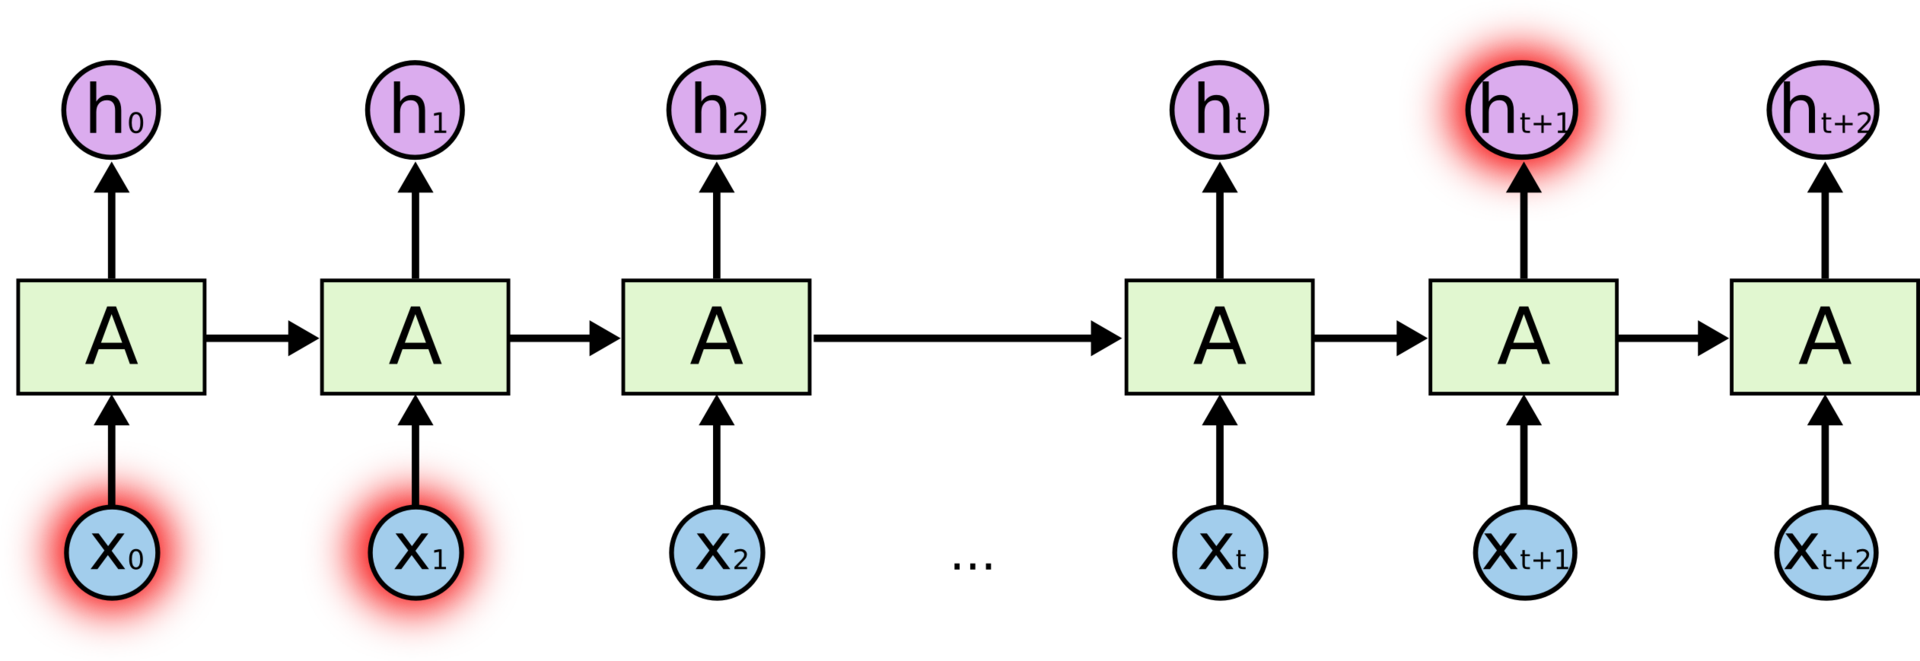
\includegraphics[width=.8\linewidth]{simple_rnn2.png}
\end{center}

\large Я вырос во Франции… Я бегло говорю по-французски
\end{frame}


\begin{frame}{Простейшая RNN}
\begin{center}
	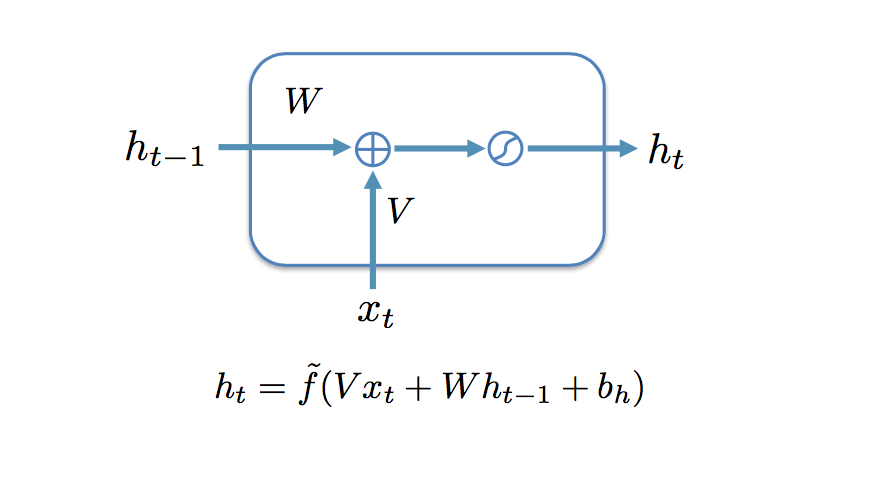
\includegraphics[width=.8\linewidth]{rnn14.png}
\end{center}
\end{frame}


\begin{frame}{Простейшая RNN}
\begin{center}
	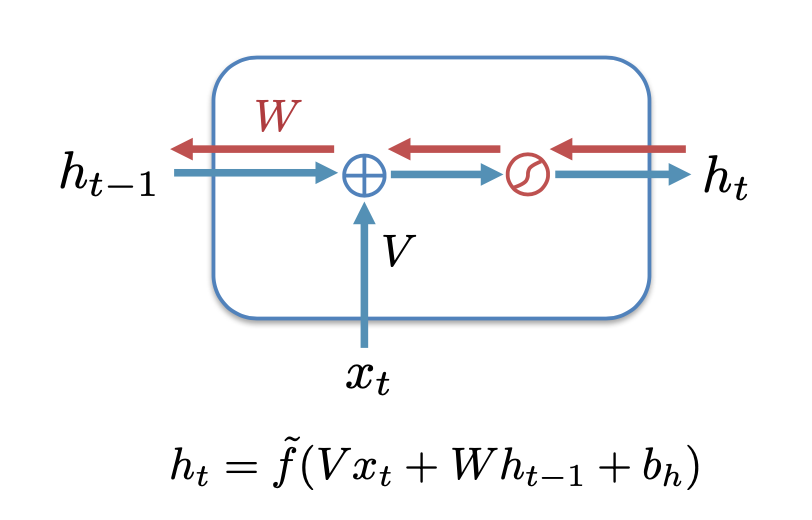
\includegraphics[width=.65\linewidth]{rnn14_2.png}
\end{center}
\end{frame}


\begin{frame}{Долгая краткосрочная память (1997)}
\begin{wideitemize}
	\item В  простой RNN-ячейке градиенты затухают из-за сложных преобразований
	\item Нужен короткий путь для градиентов 
	\item Давайте разобьём память на долгосрочной и краткосрочную и получим LSTM
\end{wideitemize}

\vspace{2.5cm}
\footnotesize 
\color{blue} \url{https://www.researchgate.net/publication/13853244\_Long\_Short-term\_Memory} 
\end{frame}


\begin{frame}{LSTM}
\begin{center}
	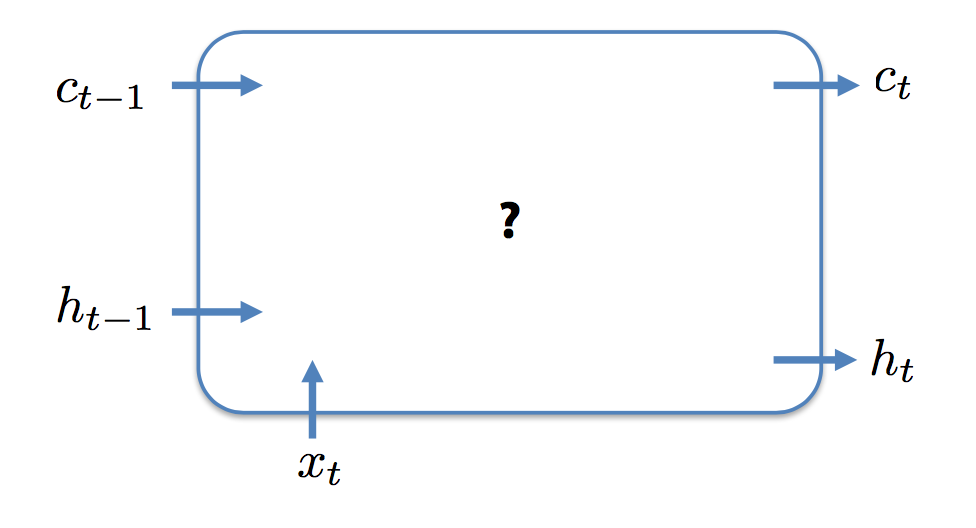
\includegraphics[width=.8\linewidth]{lstm1.png}
\end{center}
\end{frame}


\begin{frame}{LSTM}
\begin{center}
	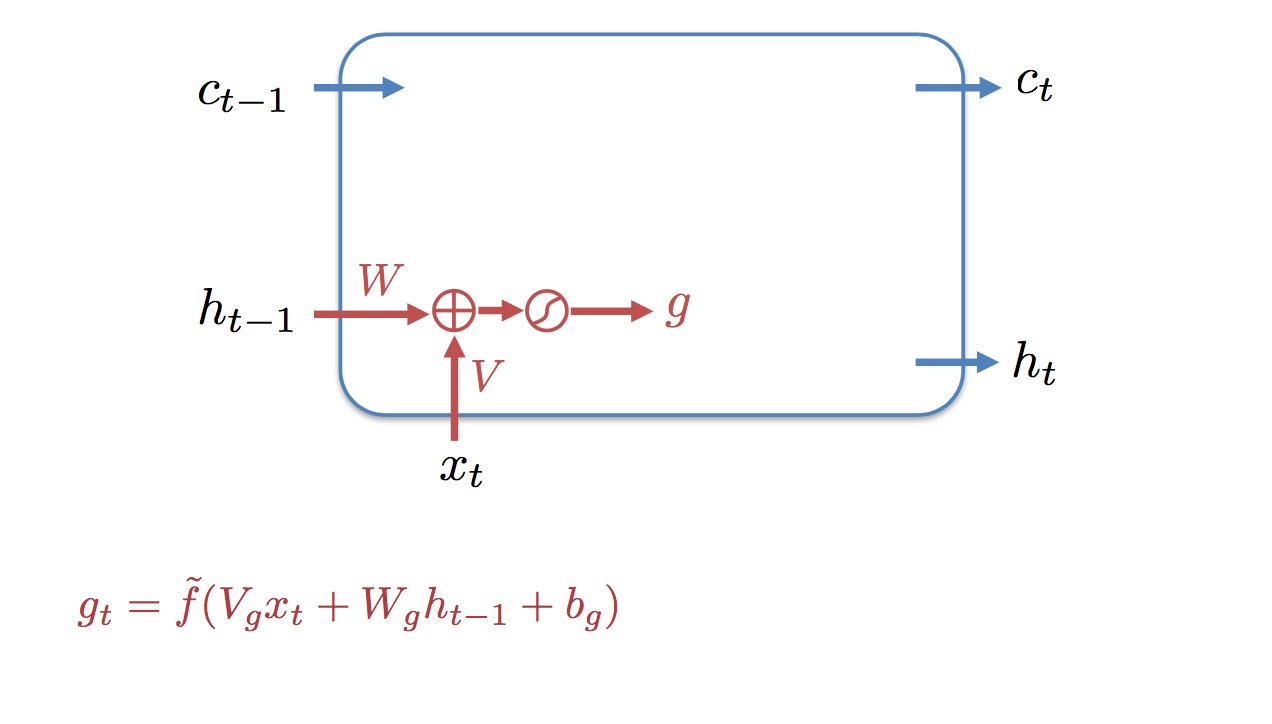
\includegraphics[width=.8\linewidth]{lstm2.png}
\end{center}
\end{frame}


\begin{frame}{LSTM}
\begin{center}
	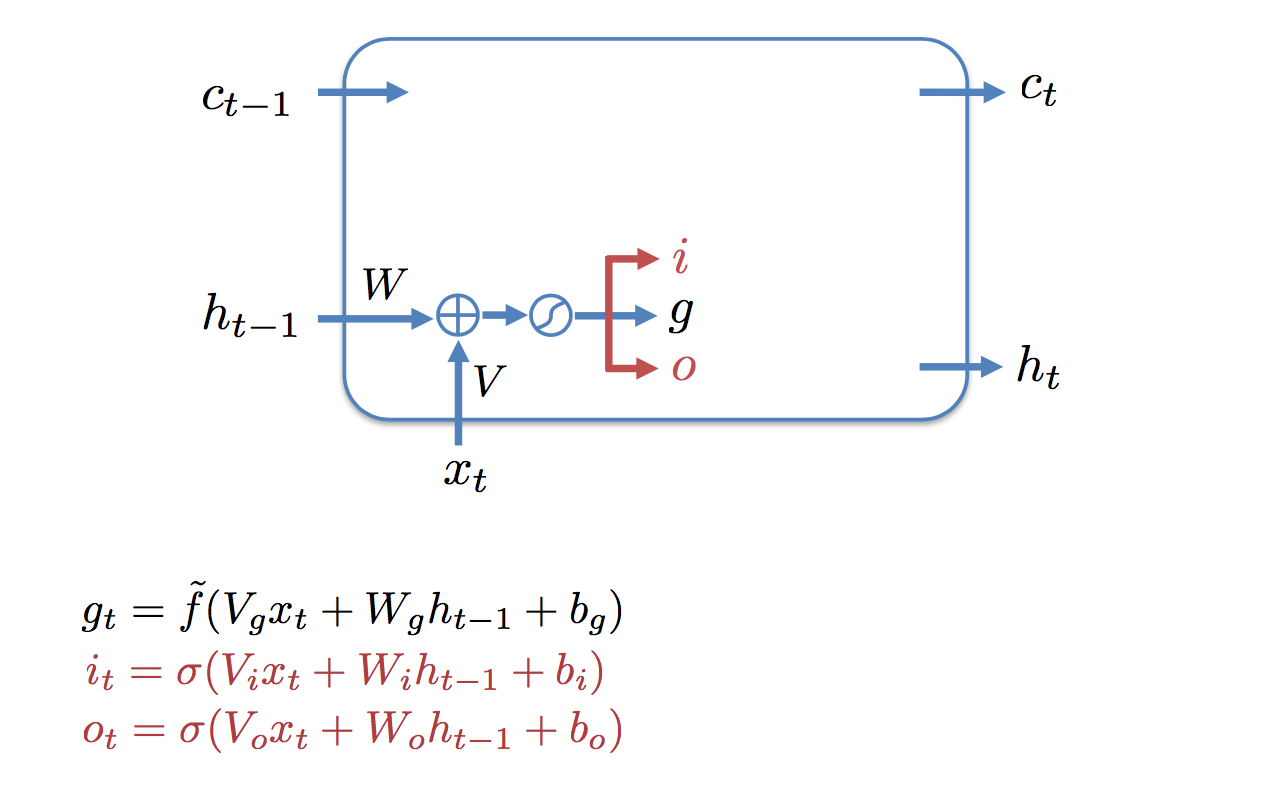
\includegraphics[width=.8\linewidth]{lstm3.png}
\end{center}
\end{frame}


\begin{frame}{LSTM}
\begin{center}
	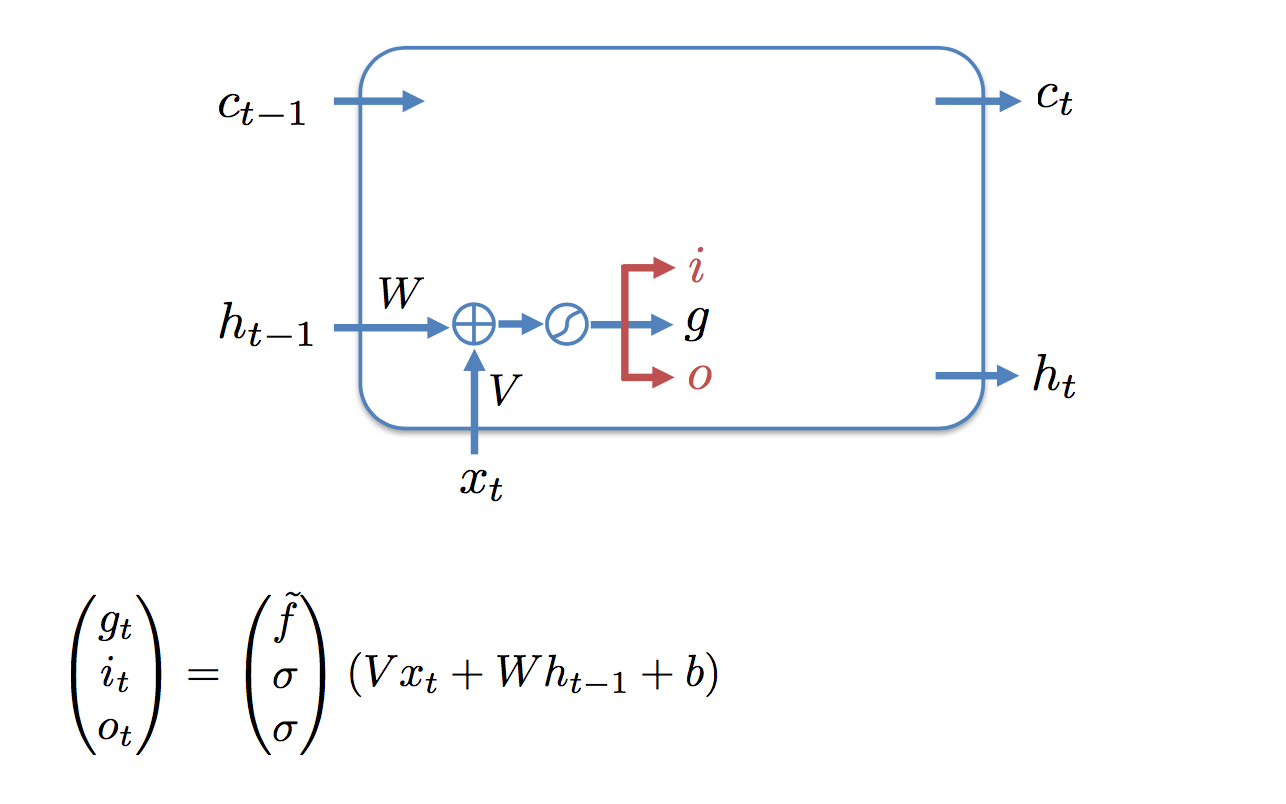
\includegraphics[width=.8\linewidth]{lstm4.png}
\end{center}
\end{frame}


\begin{frame}{LSTM}
\begin{center}
	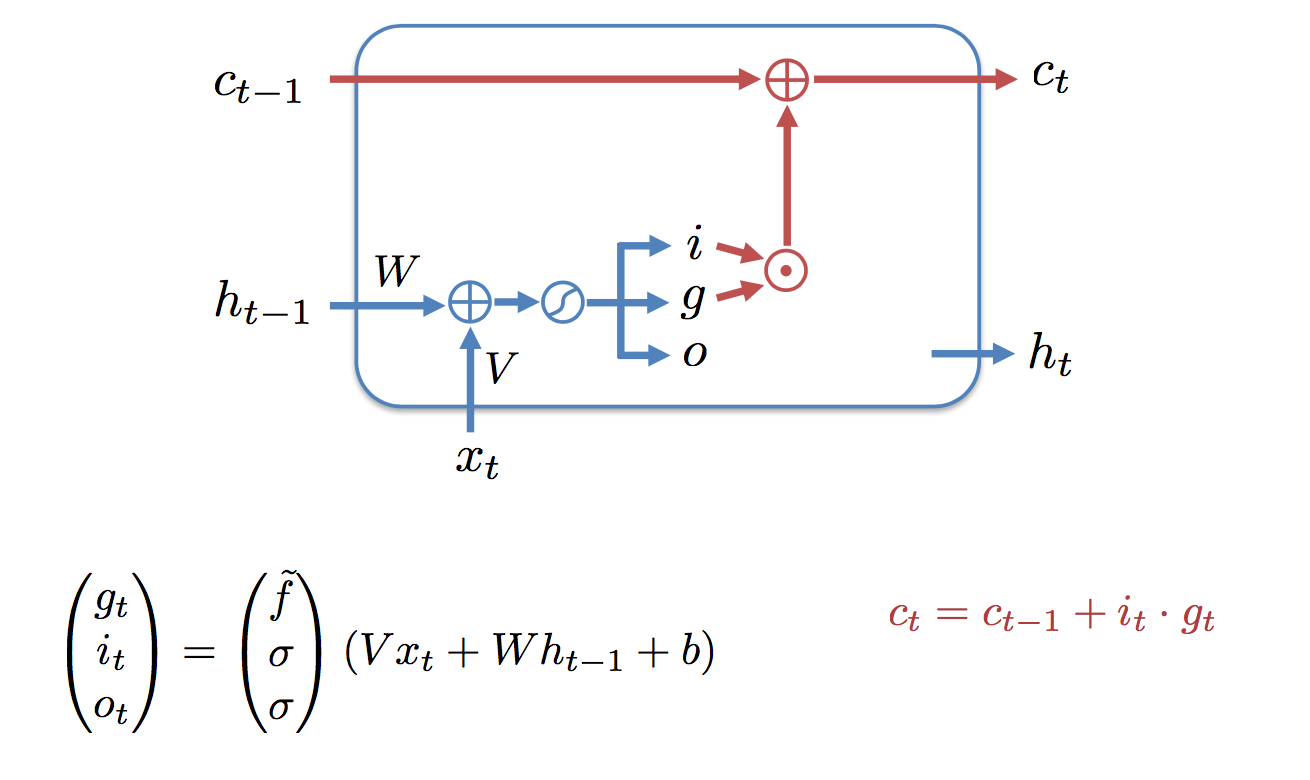
\includegraphics[width=.8\linewidth]{lstm5.png}
\end{center}
\end{frame}


\begin{frame}{LSTM}
\begin{center}
	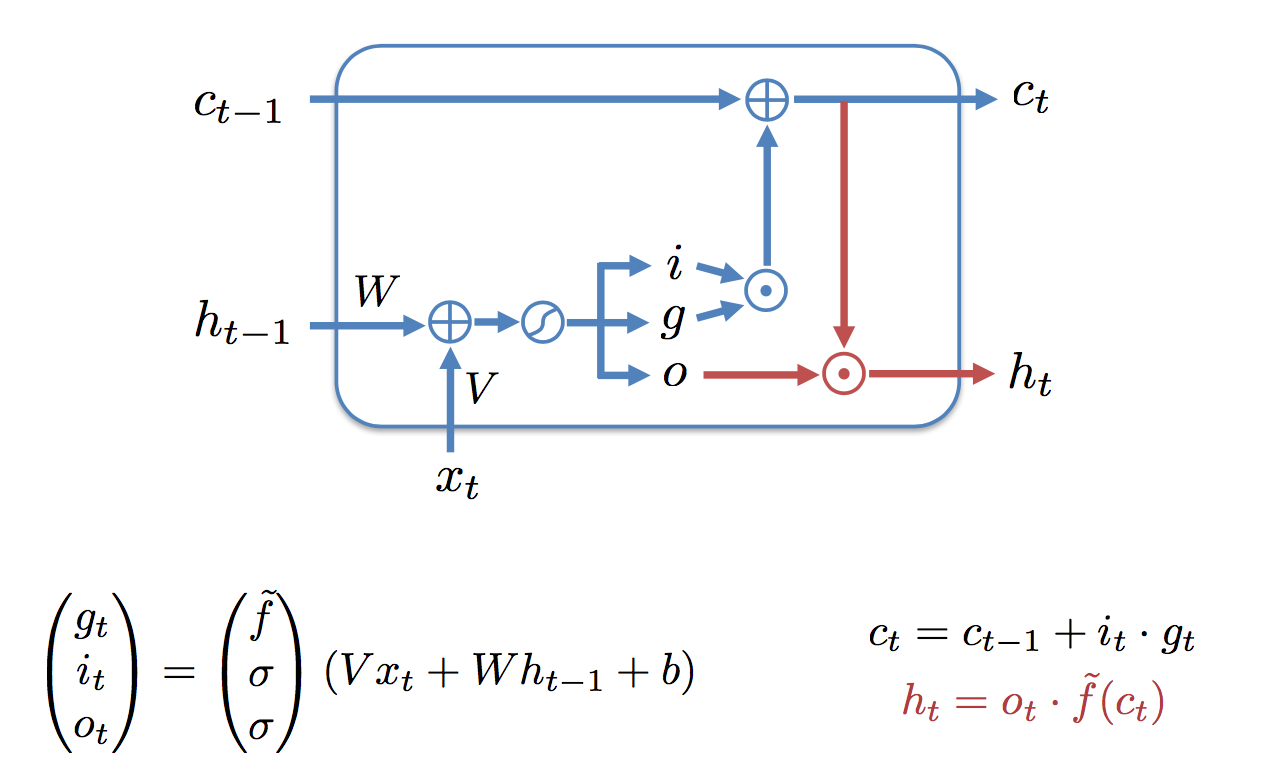
\includegraphics[width=.8\linewidth]{lstm6.png}
\end{center}
\end{frame}


\begin{frame}{LSTM}
\begin{wideitemize}
	\item  Ключевой элемент LSTM это состояние ячейки (cell state, $c_t$). Она проходит напрямую через цепочку, участвую лишь в нескольких линейных операциях. Информация может легко течь по ней не подвергаясь преобразованиям. 
	
	\item Фильтры (gates) контролируют поток информации и могут удалять лишнюю. Они состоят из слоя сигмоидальной нейронной сети и операции умножения. Сигмоида возвращает числа от $0$ до $1$, говоря какую долю информации нужно сохранить. 
	
	\item В LSTM три таких фильтра контролируют состояние ячейки. Часть забывается, часть берётся из нового входа. Все эти манипуляции делают ячейки очень гибкими. 
\end{wideitemize}
\end{frame}


\begin{frame}{LSTM}
\begin{center}
	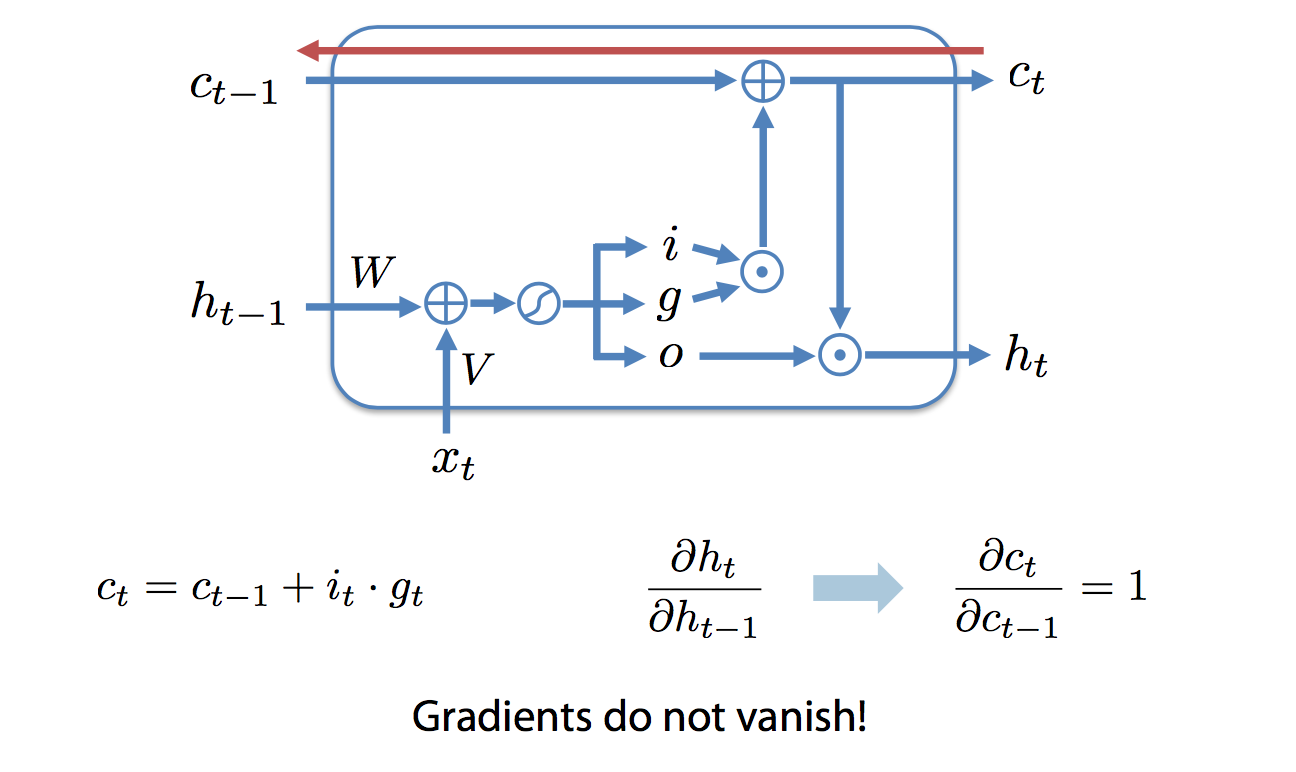
\includegraphics[width=.8\linewidth]{lstm7.png}
\end{center}
\end{frame}


\begin{frame}{LSTM}
\begin{wideitemize}
	\item  В рекурсивном вычислении состояния ячейки нет никакой нелинейности. Обычно это называют \alert{каруселью константной ошибки} 
	
	\item Ошибка в LSTM пропагируется без изменений и скрытые состояния, если LSTM сама не решит их перезаписать, могут не меняться довольно долго
	
	\item Такое устройство ячейки решает проблему исчезающих градиентов, однако проблема взрывающихся градиентов остаётся \alert{$\Rightarrow$ ограничение градиентов}
\end{wideitemize}
\end{frame}


\begin{frame}{LSTM c забыванием (1999)}
\begin{center}
	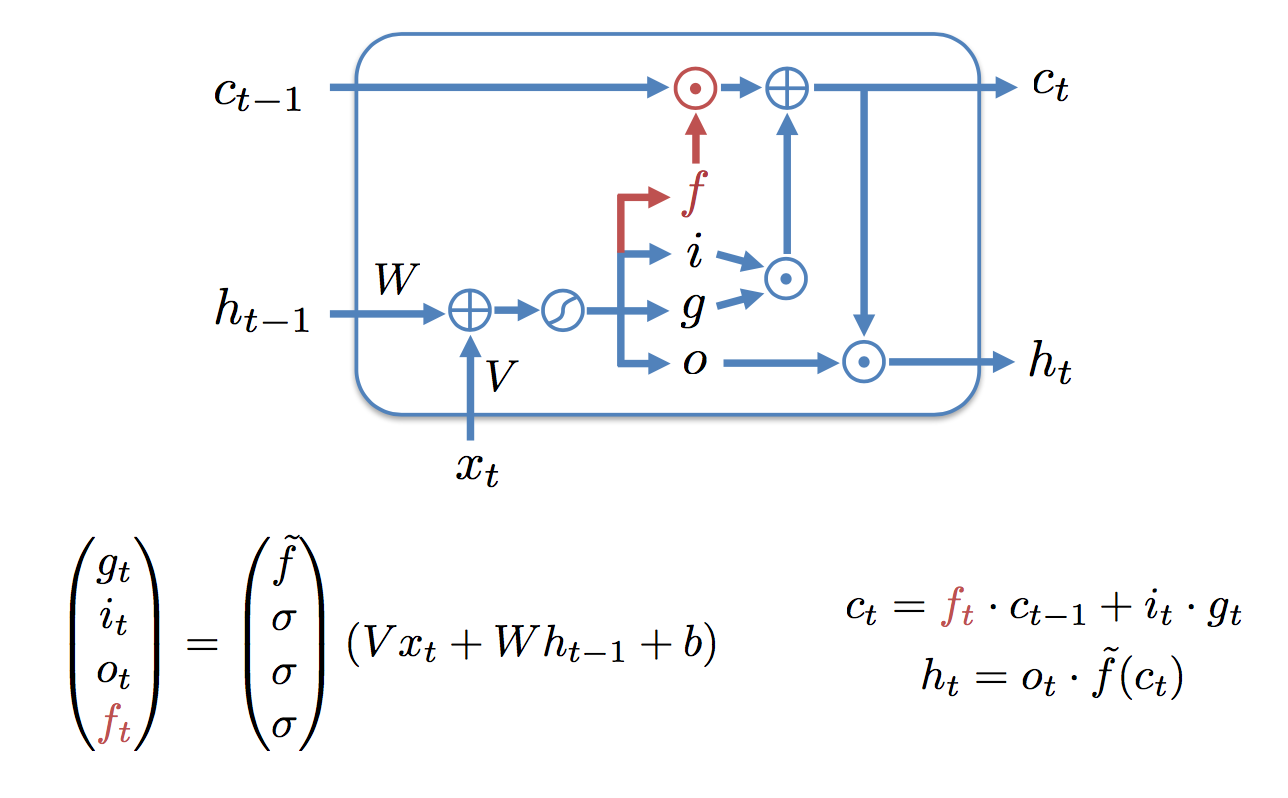
\includegraphics[width=.8\linewidth]{lstm8.png}
\end{center}
\end{frame}


\begin{frame}{LSTM c забыванием (1999)}
\begin{center}
	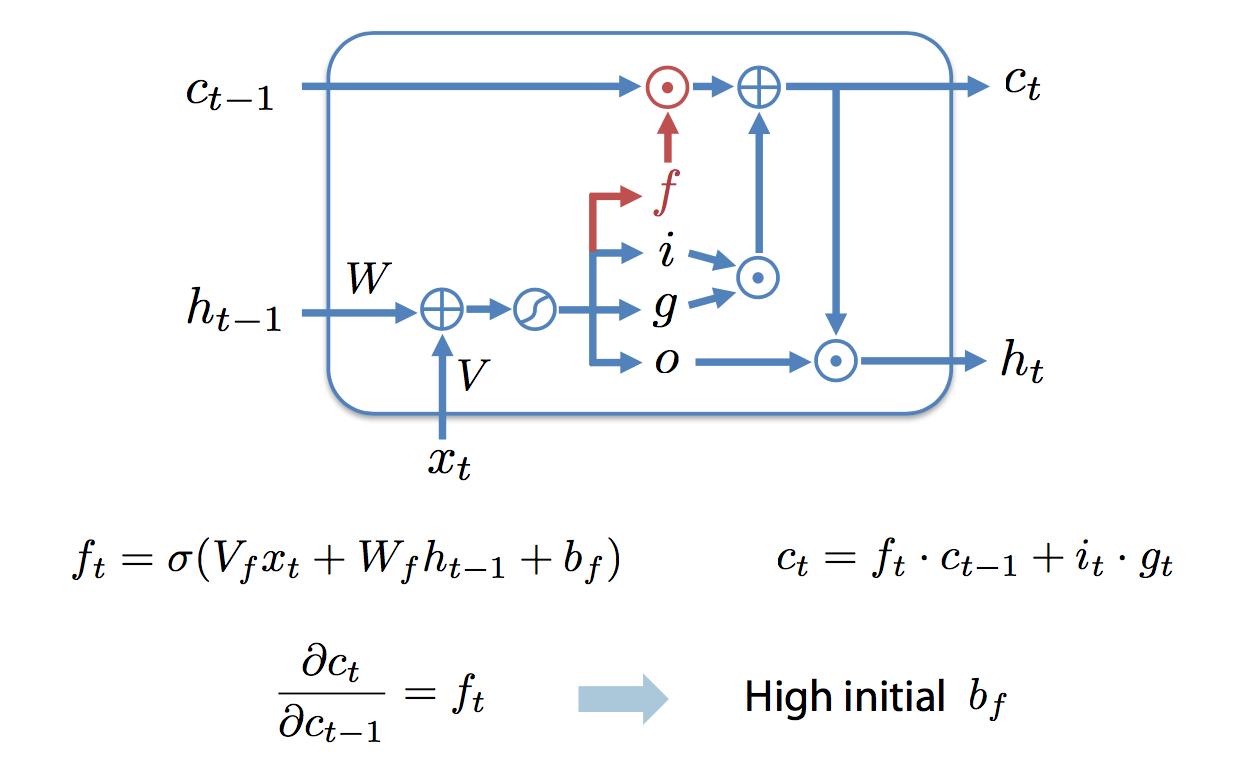
\includegraphics[width=.8\linewidth]{lstm9.png}
\end{center}
\end{frame}


\begin{transitionframe}
	\begin{center}
		\Huge GRU 
	\end{center}
%\centering 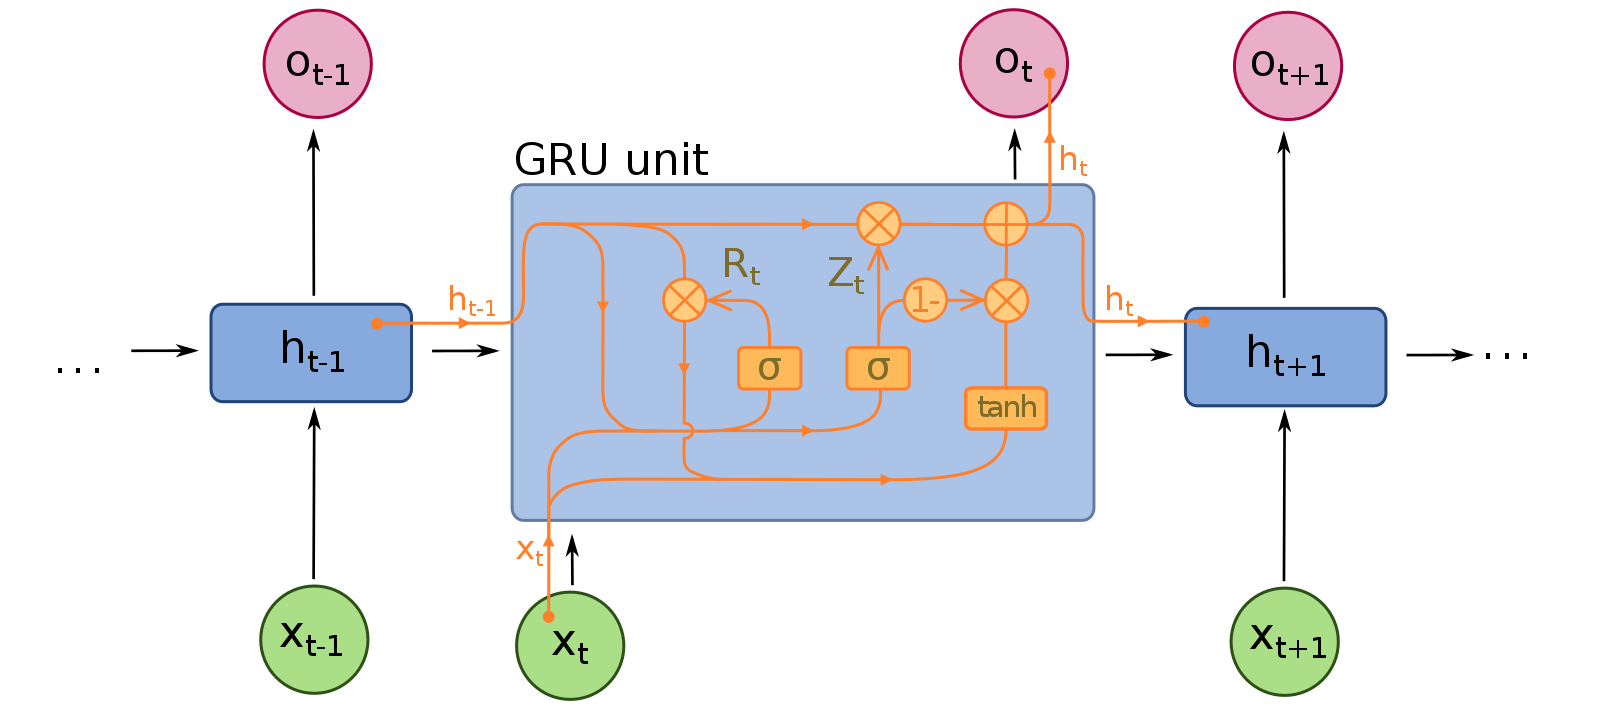
\includegraphics[scale = 0.15]{gru-start.png}
\centering 
\includegraphics[scale = 0.25]{gru-ahah.png}
\end{transitionframe}


\begin{frame}{А вот бы весов поменьше бы}
\begin{wideitemize}
	\item  В 2015 году придумали GRU-ячейку
	
	\item Придумали с желанием сохранить память в ячейке, но упростить LSTM
	
	\item Учиться и применяется на 20-50\% быстрее, результаты в большинстве случаев похожие
\end{wideitemize}
\end{frame}

\begin{frame}{GRU-ячейка}
\begin{center}
	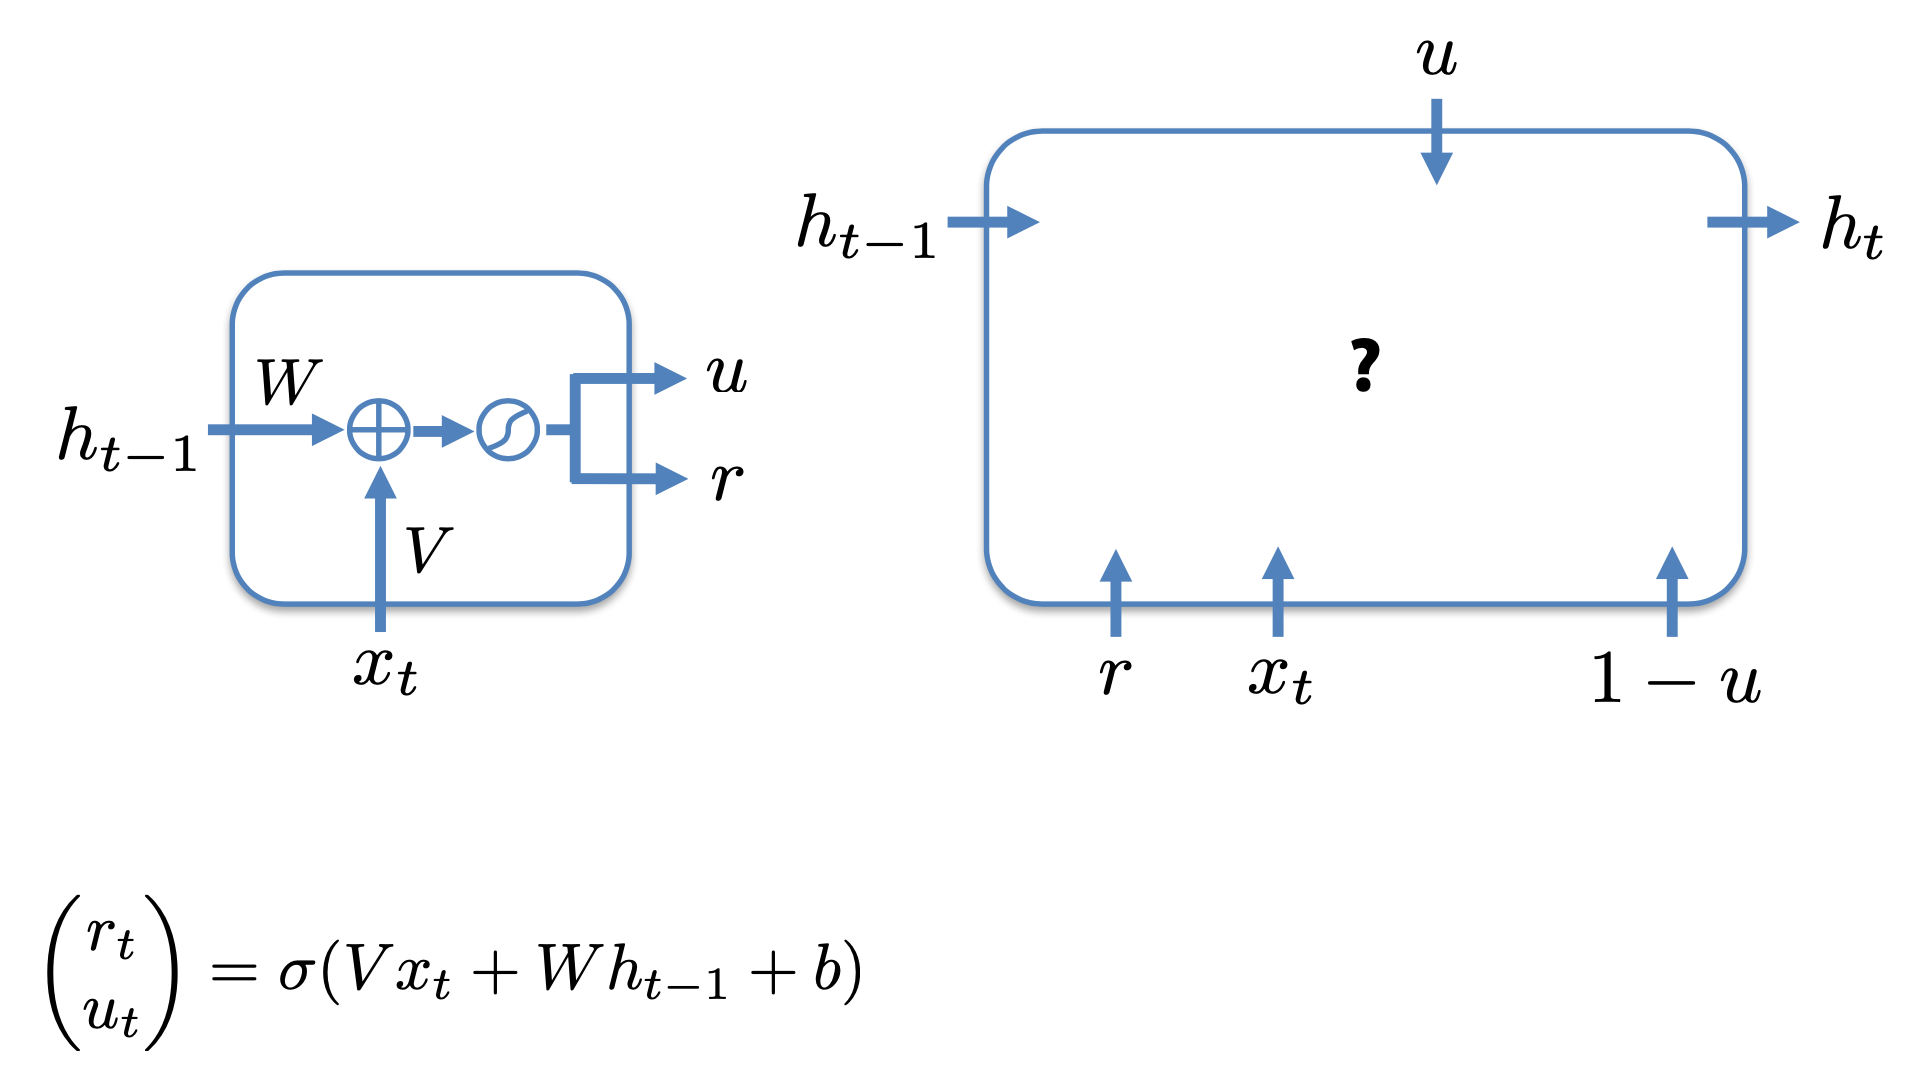
\includegraphics[width=.8\linewidth]{gru1.png}
\end{center}
\end{frame}

\begin{frame}{GRU-ячейка}
\begin{center}
	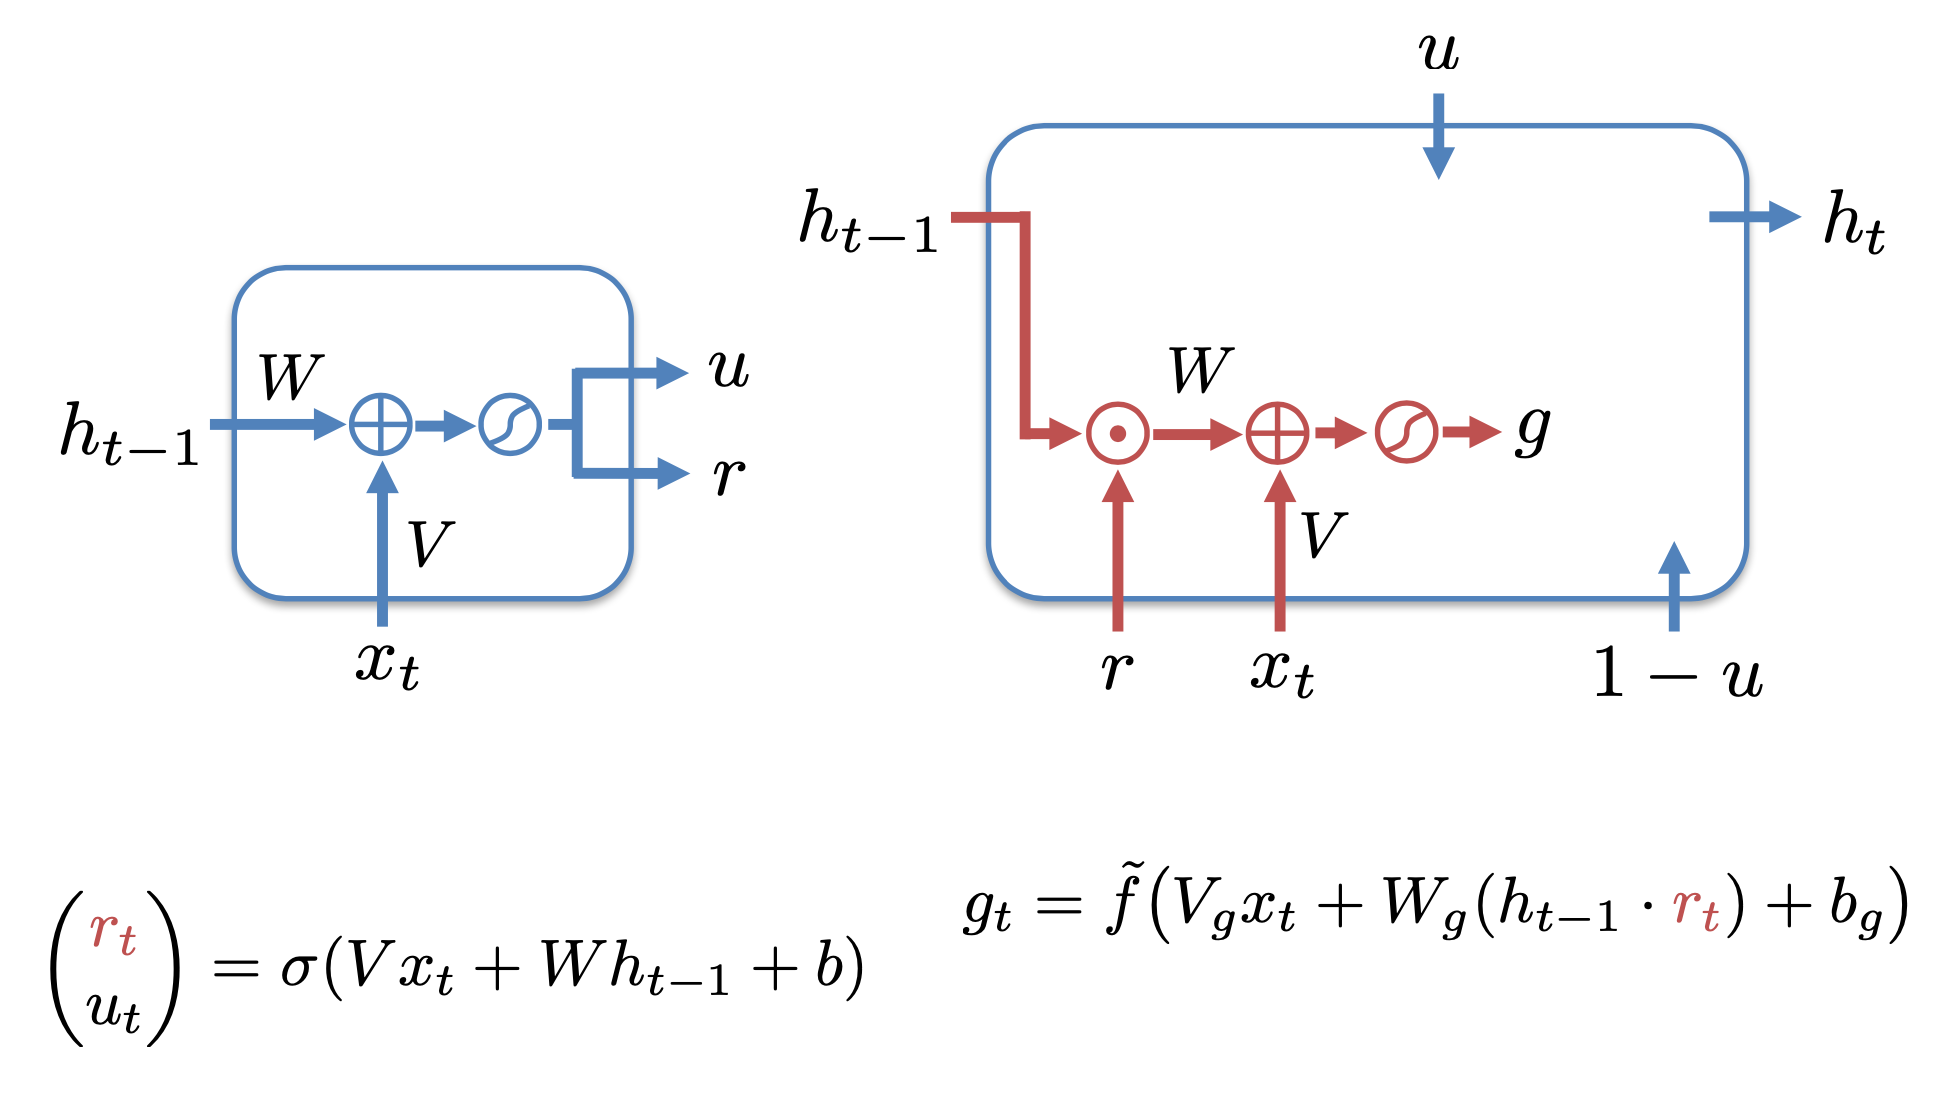
\includegraphics[width=.8\linewidth]{gru2.png}
\end{center}
\end{frame}

\begin{frame}{GRU-ячейка}
\begin{center}
	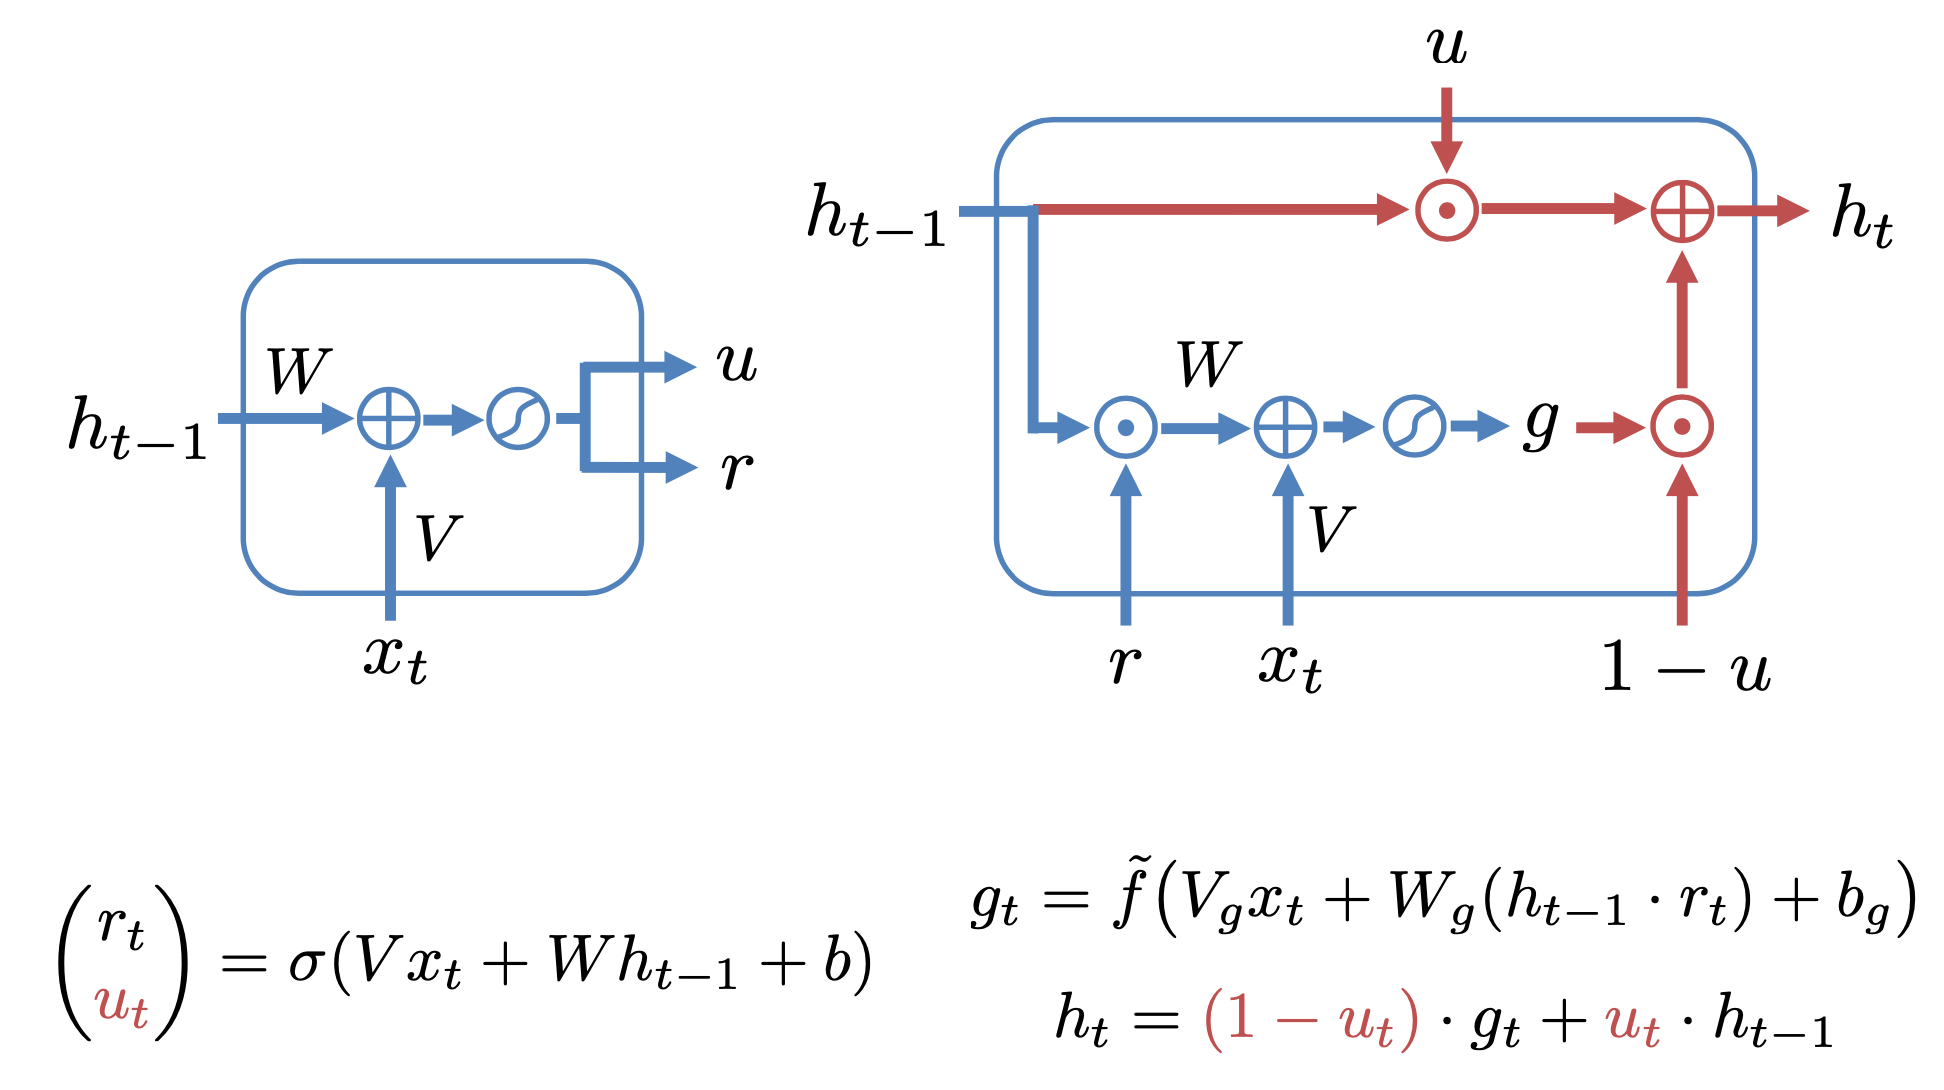
\includegraphics[width=.8\linewidth]{gru3.png}
\end{center}
\end{frame}

\begin{frame}{GRU-ячейка}
\begin{center}
	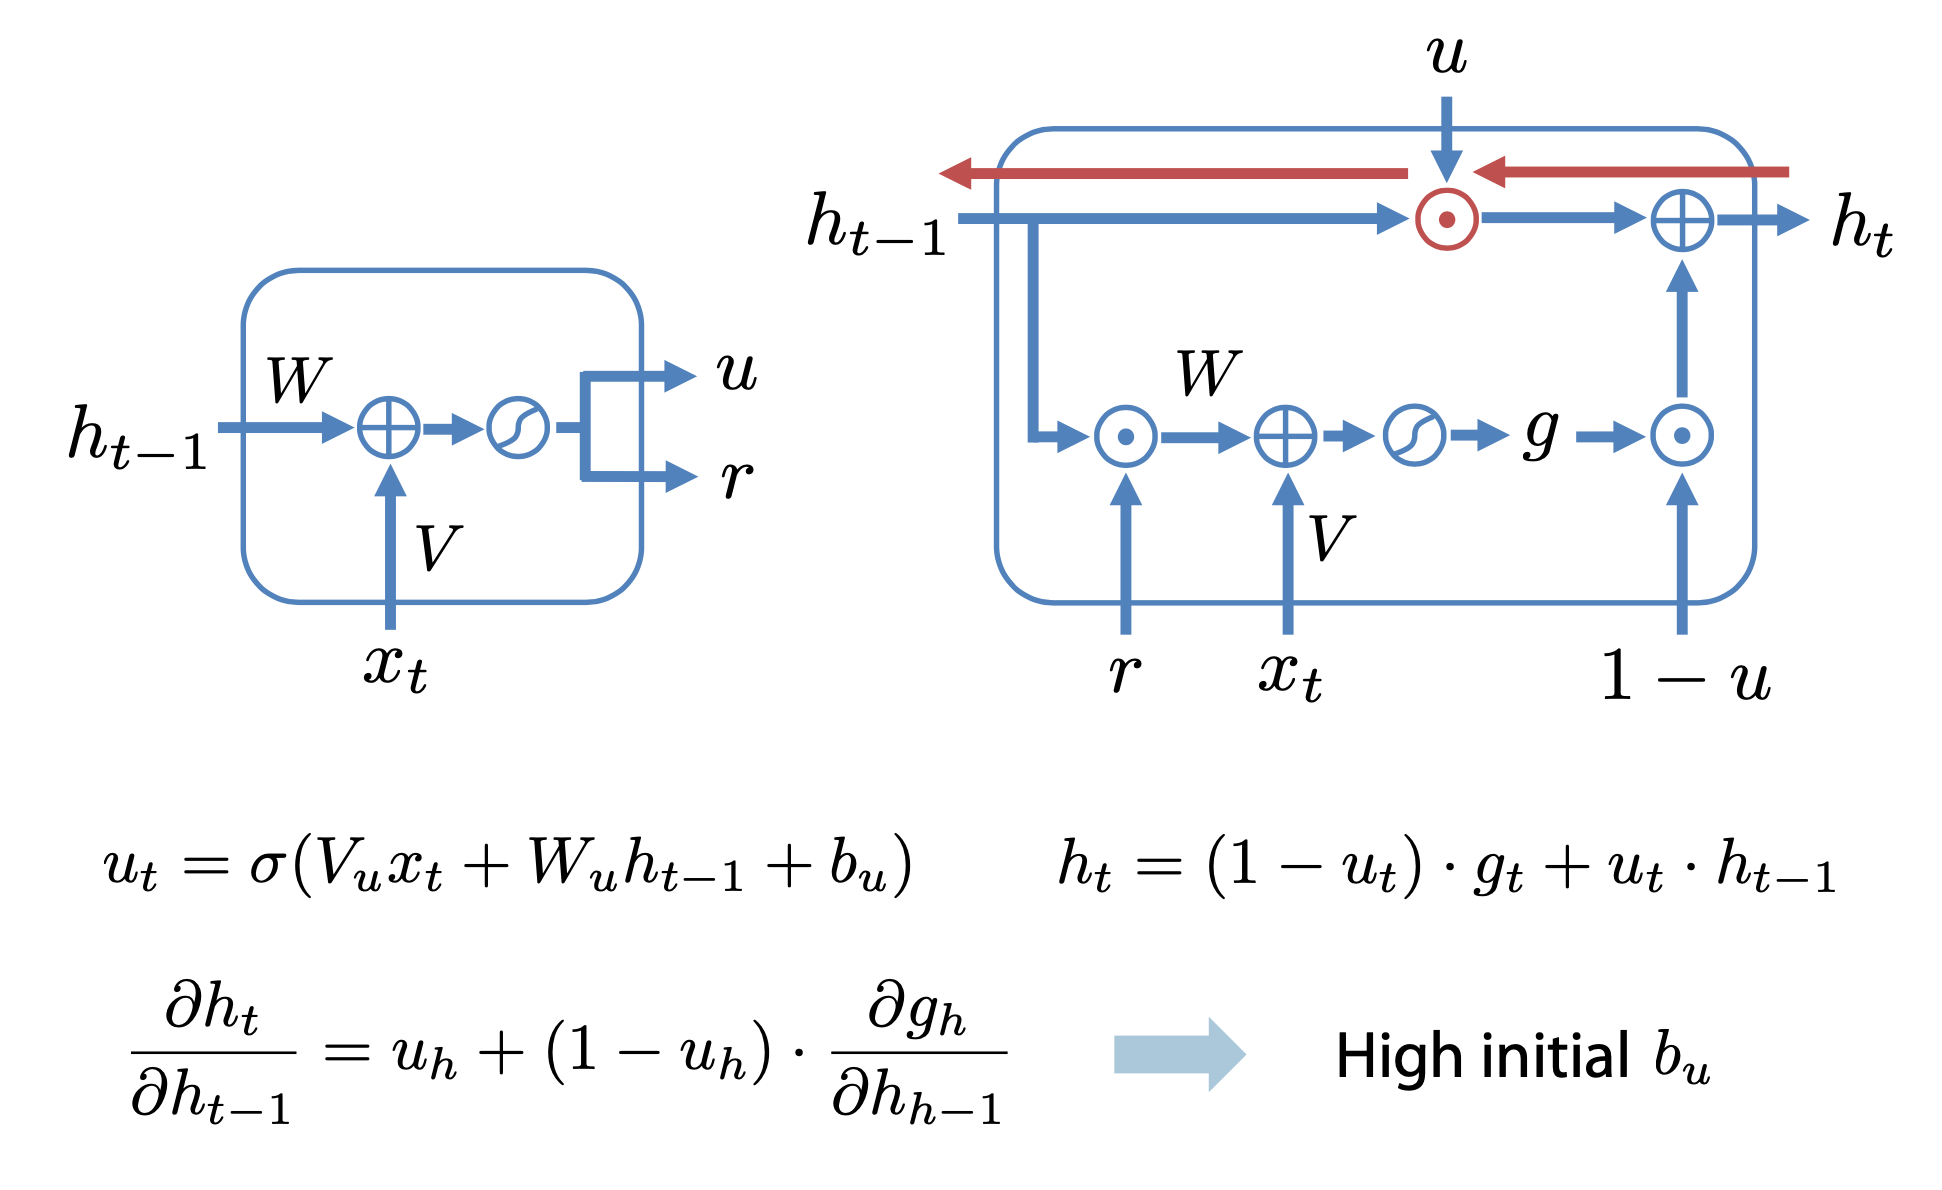
\includegraphics[width=.8\linewidth]{gru4.png}
\end{center}
\end{frame}


\begin{frame}{Помоги Google найти новую ячейку (2015)}
\begin{columns}
	\begin{column}{.55\linewidth}
		\begin{itemize} 
			\item  LSTM и GRU придуманы из головы, нет гарантии их оптимальности
			\item  Google решил сделать перебор $10000$ разных ячеек
			\item  Нашли новые ячейки похожие на LSTM и GRU
		\end{itemize}
	\begin{center}
		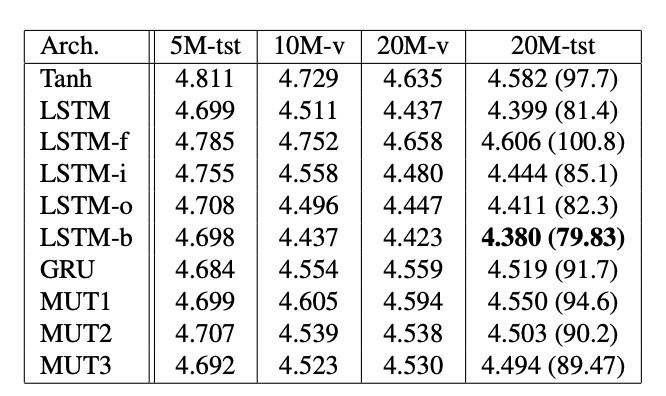
\includegraphics[width=.65\linewidth]{google-cell2.png}
	\end{center}
	\end{column}	
	\begin{column}{.45\linewidth}			
		\begin{center}
			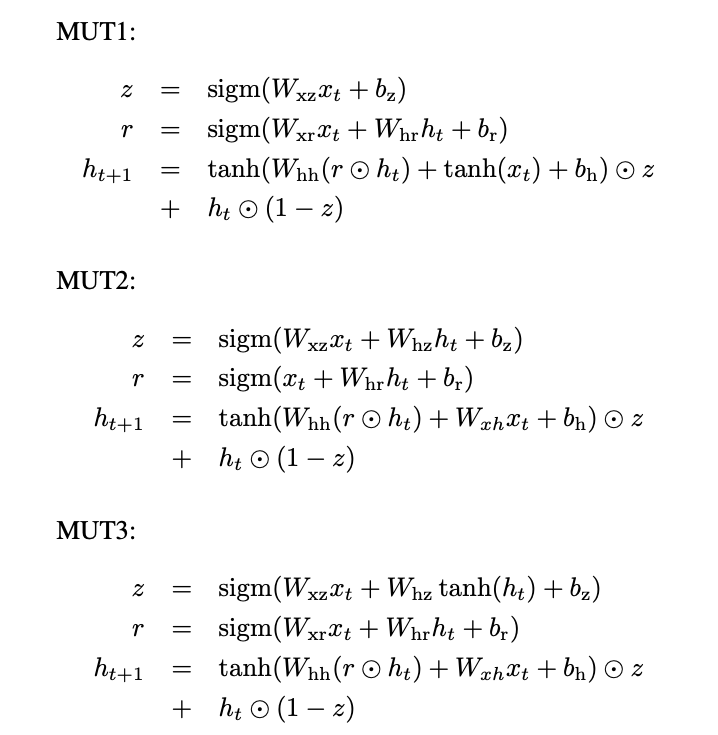
\includegraphics[width=.99\linewidth]{google_cell.png}
		\end{center}
	\end{column}	
\end{columns}
\vfill 
\footnotesize 
\color{blue} \url{http://proceedings.mlr.press/v37/jozefowicz15.pdf} 
\end{frame}


\begin{transitionframe}
	\begin{center}
		\Huge Двунаправленные рекуррентные сети
	\end{center}
\centering 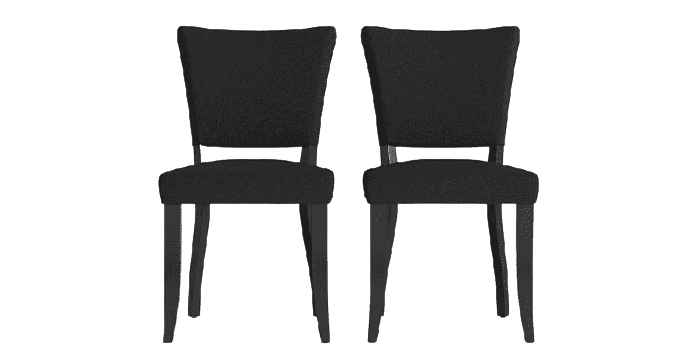
\includegraphics[scale = 0.25]{twochair.png}
\end{transitionframe}


\begin{frame}{Двунаправленные рекуррентные сети}
\begin{center}
	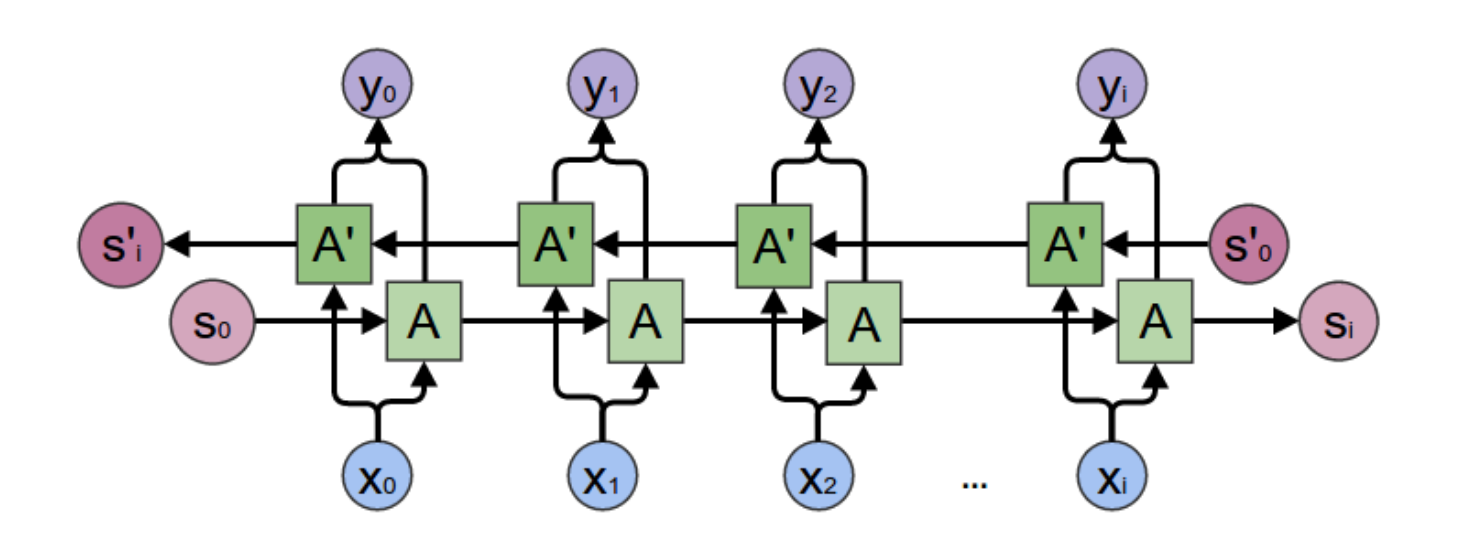
\includegraphics[width=.9\linewidth]{biderect_lstm.png}
\end{center}
\end{frame}


\begin{frame}{Двунаправленные рекуррентные сети}
\begin{wideitemize}
	\item  Часто RNN к концу последовательности забывает о том, с чего всё начиналось, последние элементы последовательности всегда будут важнее первых 
	
	\item Давайте один слой будет читать последовательность слева направо, а второй справа налево.  Разумеется это можно делать только для тех последовательностей, которые даны нам целиком (предложения, аудио)  и нельзя для тех, которые мы видим только в прошлое (валютный курс).
	
	\item Для каждого элемента получаем скрытое состояние, отражающее его контекст и слева и справа.
\end{wideitemize}
\end{frame}


\begin{frame}{Достоинства RNN}
\begin{wideitemize}
	{\color{green}
	\item  Может обрабатывать ввод любой длины
	\item  Вычисление для шага $t$ может (теоретически) использовать информацию из всей последовательности}
	{\color{red}	
	\item Вычисления работают очень долго, градиенты могут взрываться
	\item Получить информацию со всей последовательности очень сложно}
\end{wideitemize}
\end{frame}


%\begin{transitionframe}
%	\begin{center}
%		\Huge Попробуем применить рекуррентные сети к временным рядам в python!
%	\end{center}
%\end{transitionframe}

%\begin{transitionframe}
%	\begin{center}
%		\Huge Кросс-валидация для временных рядов 
%	\end{center}
%\end{transitionframe}
%
%
%\begin{frame}{Cross validation on a rolling basis}
%	\begin{center}
%		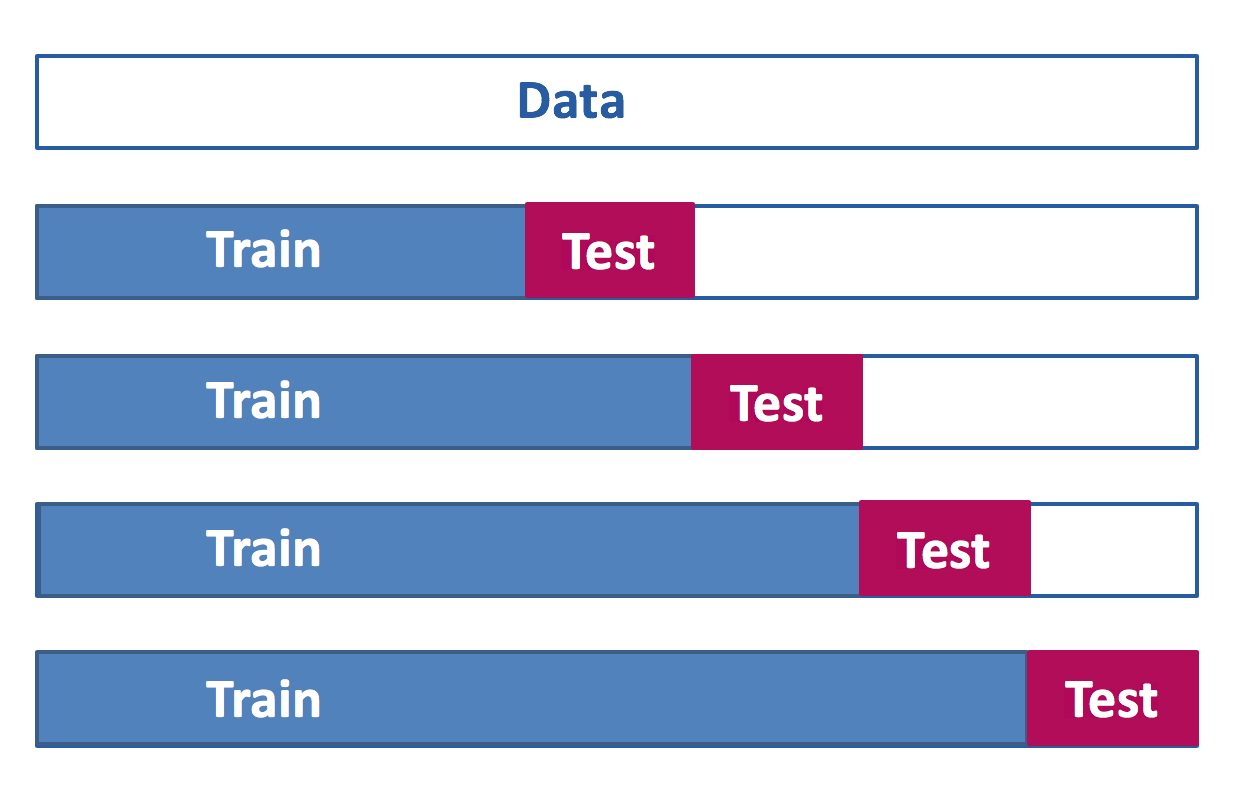
\includegraphics[width=.7\linewidth]{cv1.png}
%	\end{center}
%\end{frame}
%
%
%\begin{frame}{Cross validation on a rolling basis}
%	\begin{center}
%		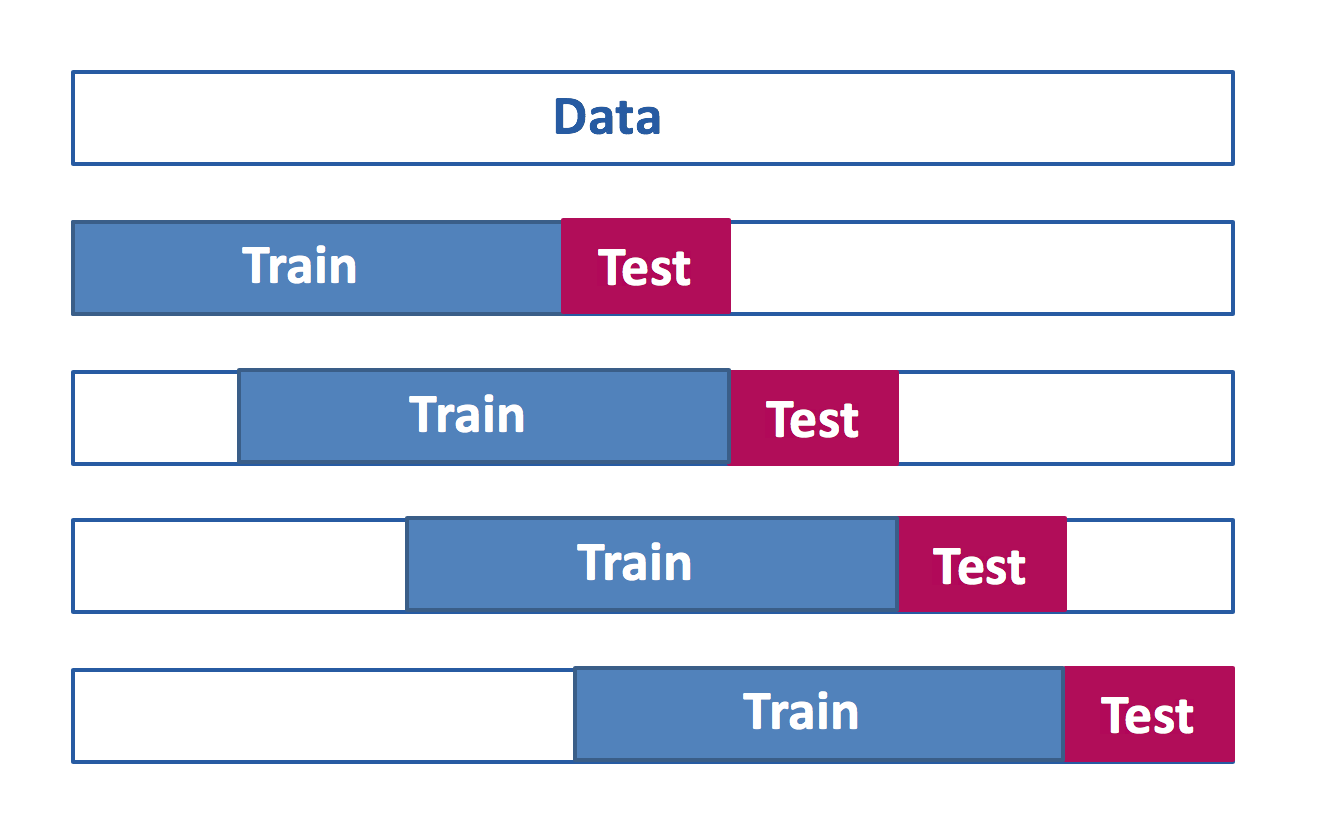
\includegraphics[width=.7\linewidth]{cv2.png}
%	\end{center}
%\end{frame}
%
%
%\begin{frame}{Cross validation on a rolling basis}
%	\begin{wideitemize}
%		\item  \alert{Leave one out кросс-валидация} – когда в тест берём каждый раз только одно, следующее наблюдение
%		\item Нельзя приравнивать разные горизонты прогнозирования 
%		\item Модель может хорошо прогнозировать на неделю вперёд, но при этом плохо прогнозировать на месяц вперёд, либо наоборот 
%		\item Иногда метрики вычисляют для разных горизонтов прогнозирования отдельно
%	\end{wideitemize}
%\end{frame}



\end{document}
